In this appendix 2D templates at \mHi = 160 \GeV~and 200 \GeV~are shown.

%%%%%% mH=160 GeV
\begin{figure}[!hbtp]
	
	%
	\centering
	\subfigure[Signal]{
	\centering
	\label{subfig:template_signal_160}
		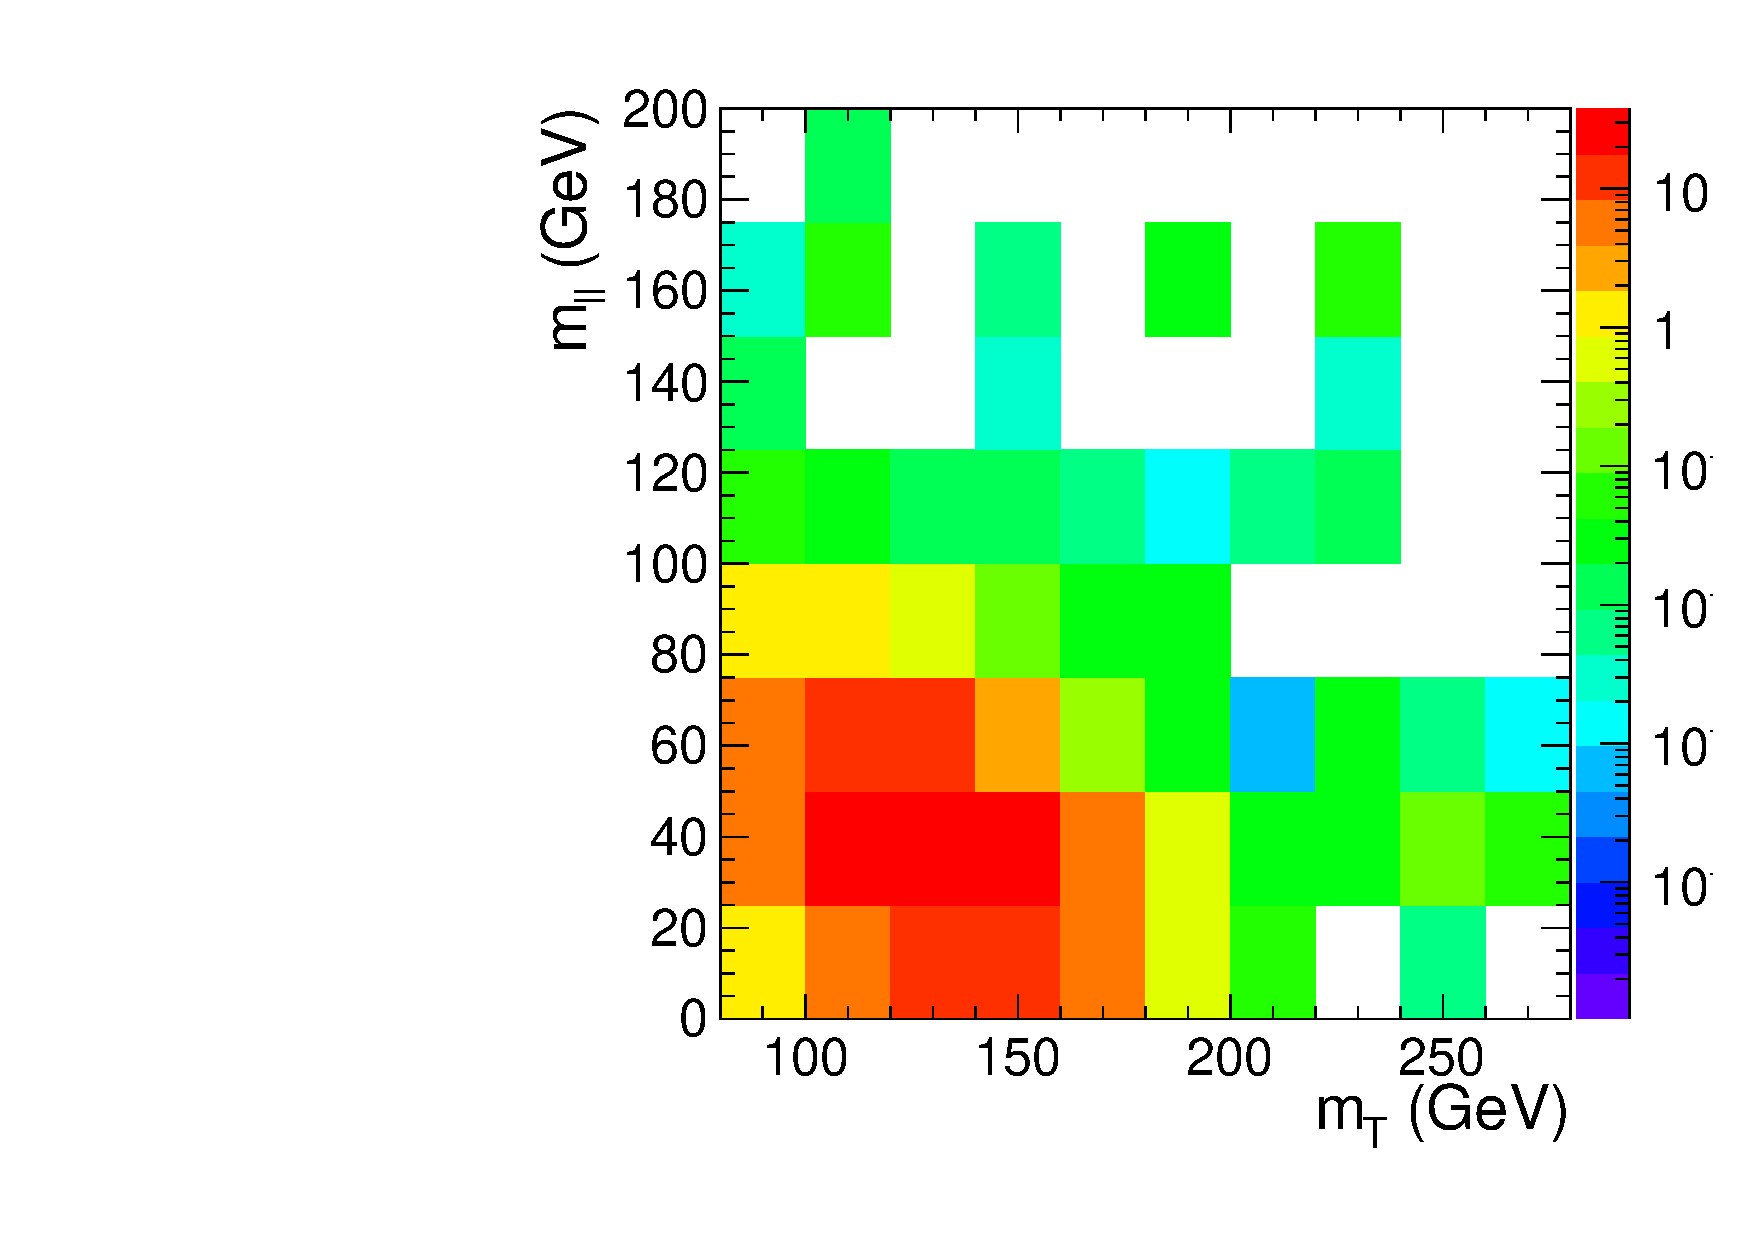
\includegraphics[width=.35\textwidth]{figures/templates/sig_2D_mH160_0j_of.pdf}
	}
	\subfigure[Signal statistical uncertainty]{
	\centering
	\label{subfig:template_signalerr_160}
		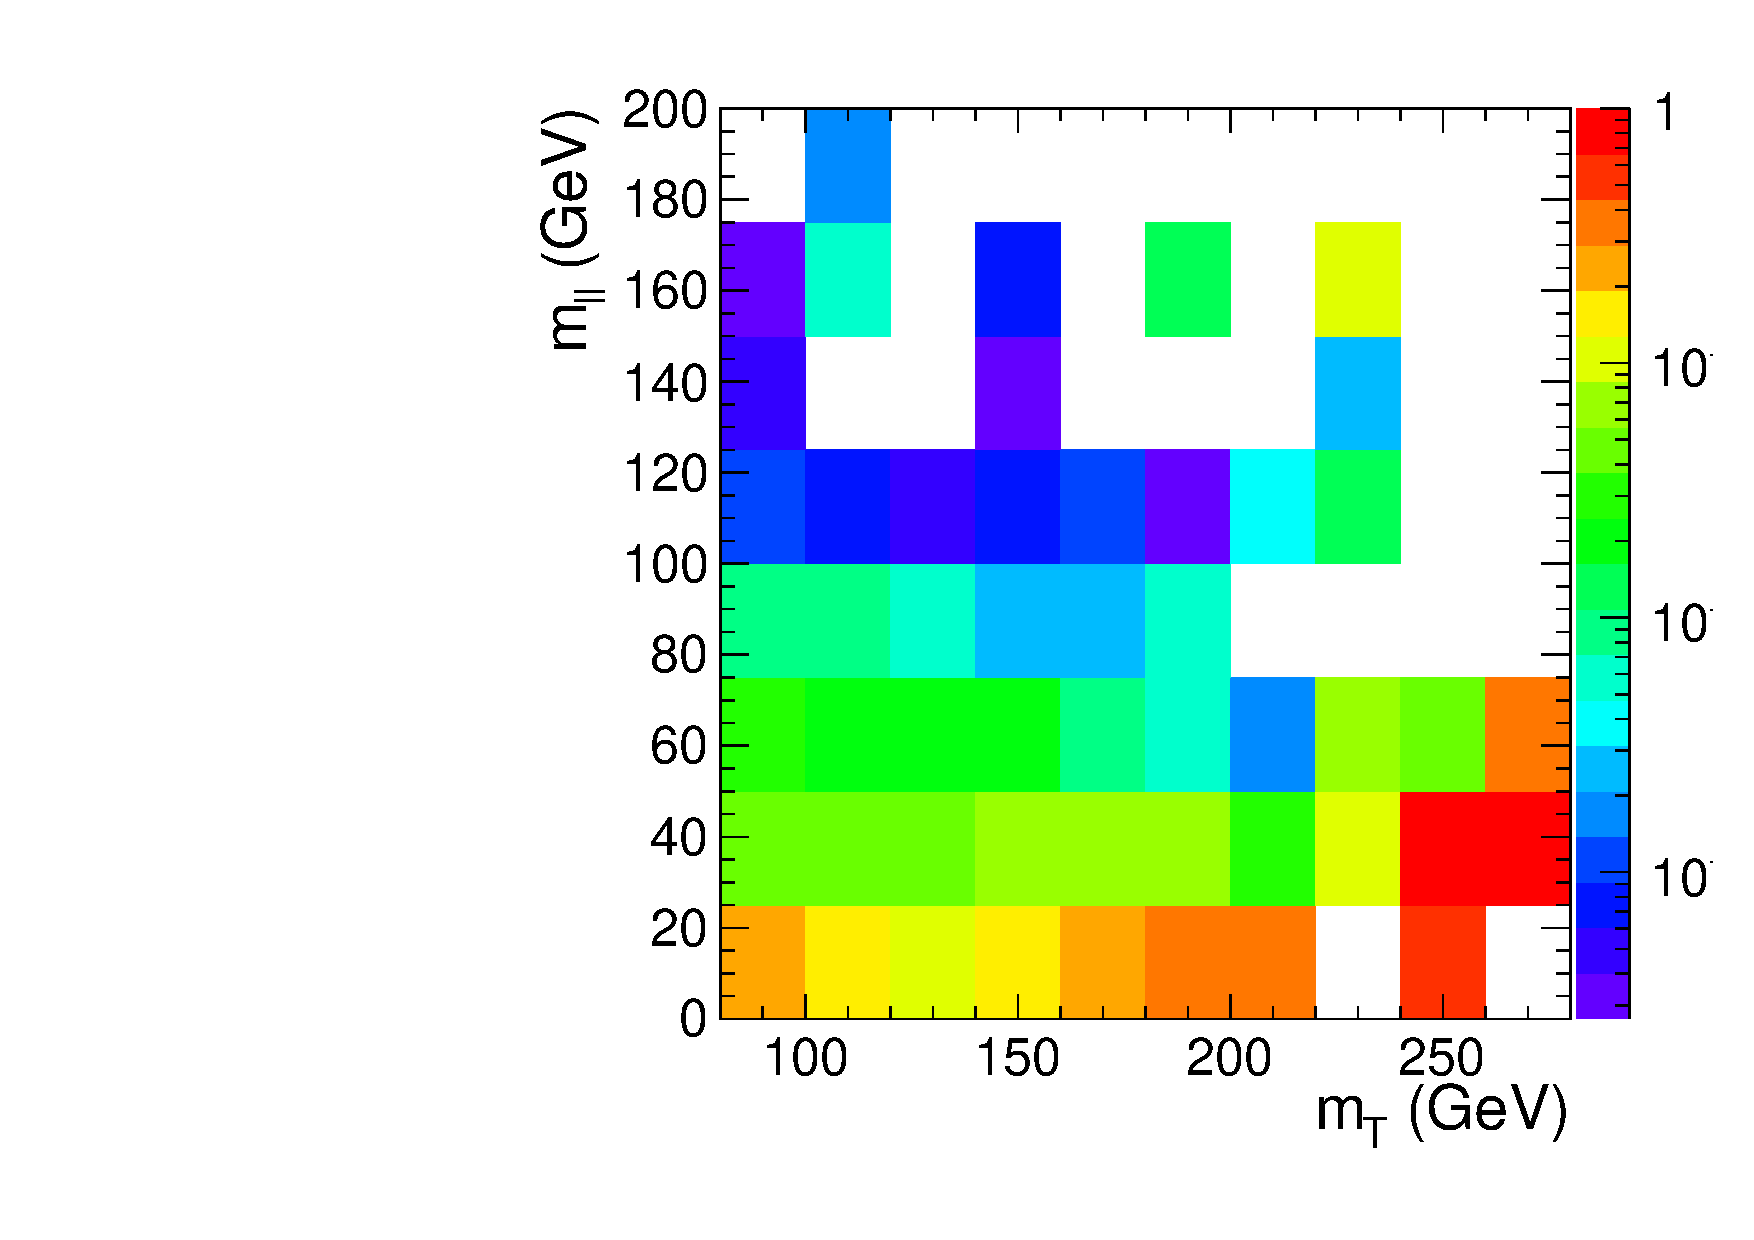
\includegraphics[width=.35\textwidth]{figures/templates/sigerr_2D_mH160_0j_of.pdf}
	}
	
	%
	\centering
	\subfigure[qqWW]{
	\centering
	\label{subfig:template_qqWW_160}
		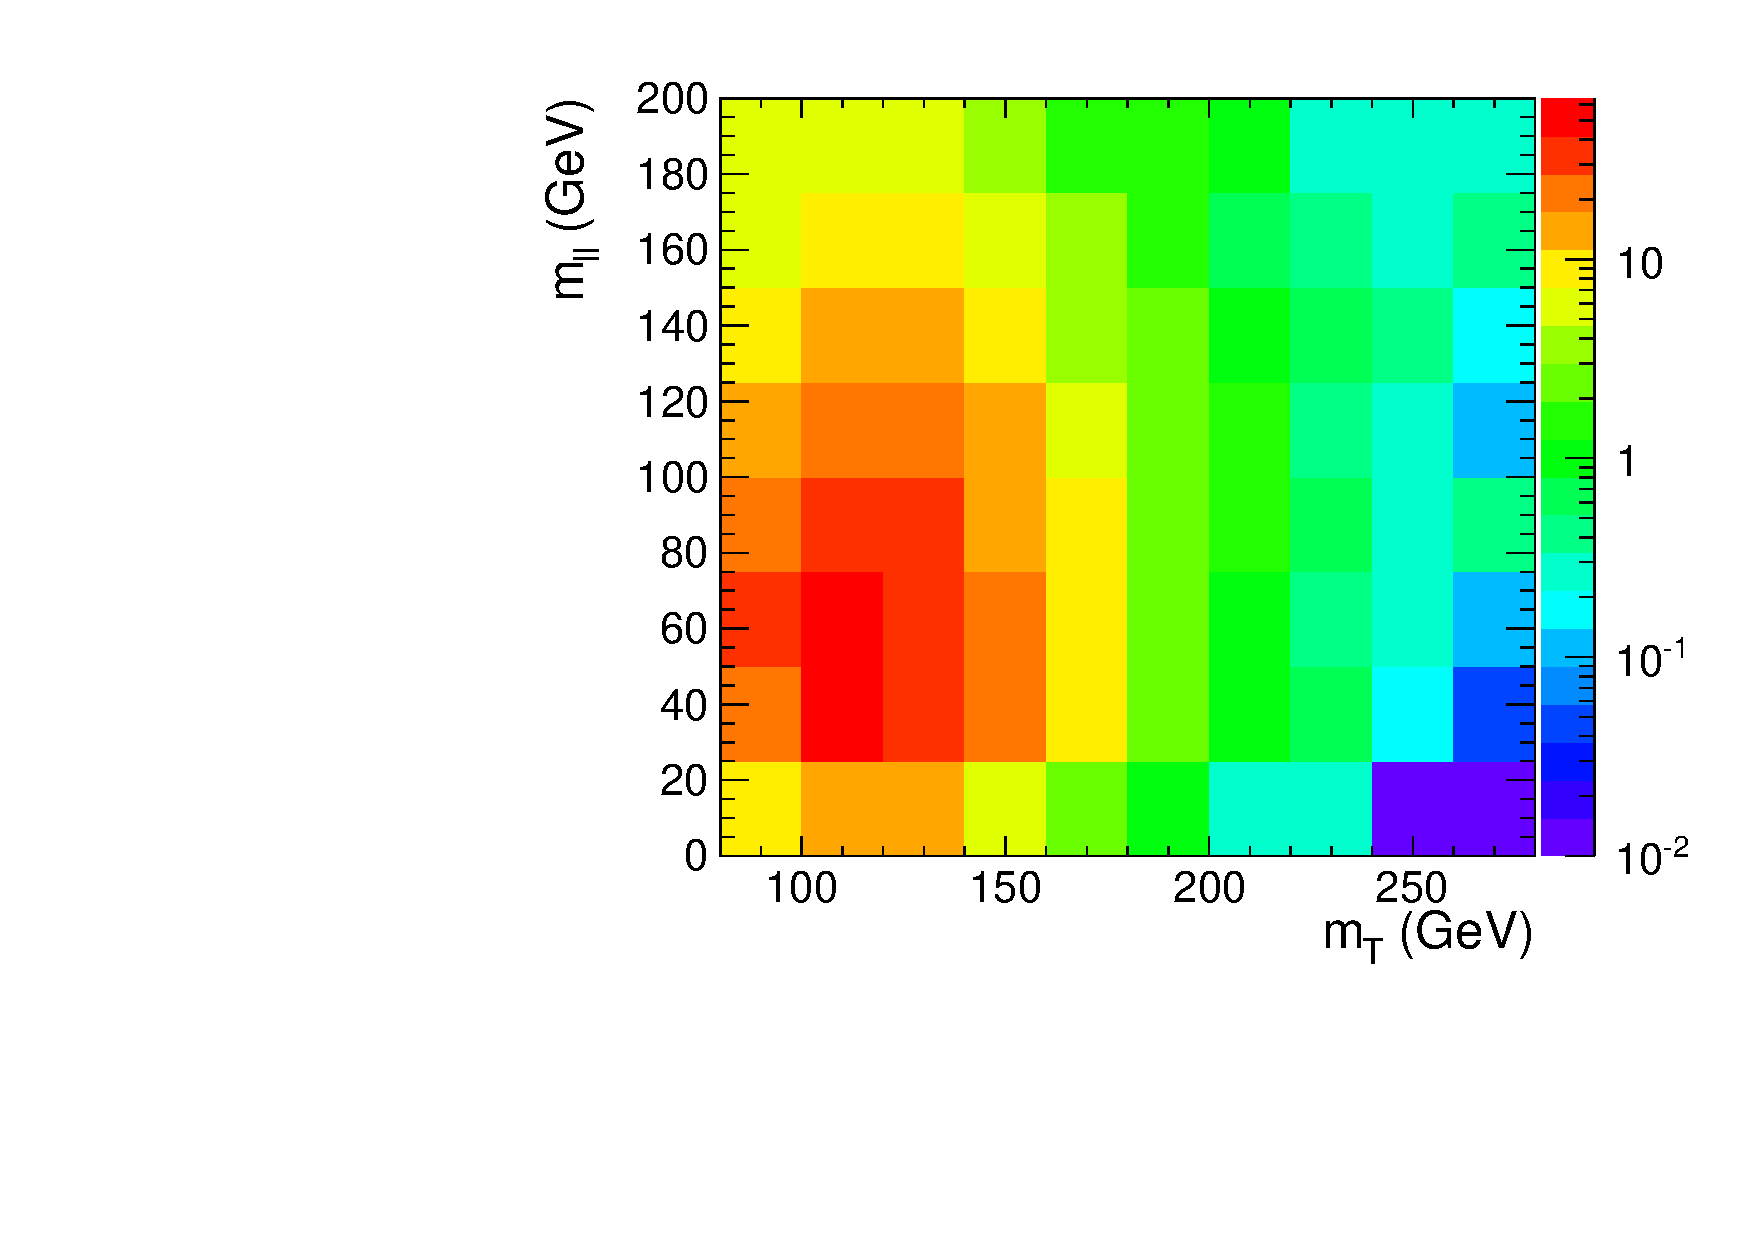
\includegraphics[width=.35\textwidth]{figures/templates/qqWW_2D_mH160_0j_of.pdf}
	}
	\subfigure[qqWW statistical uncertainty]{
	\centering
	\label{subfig:template_qqWWerr_160}
		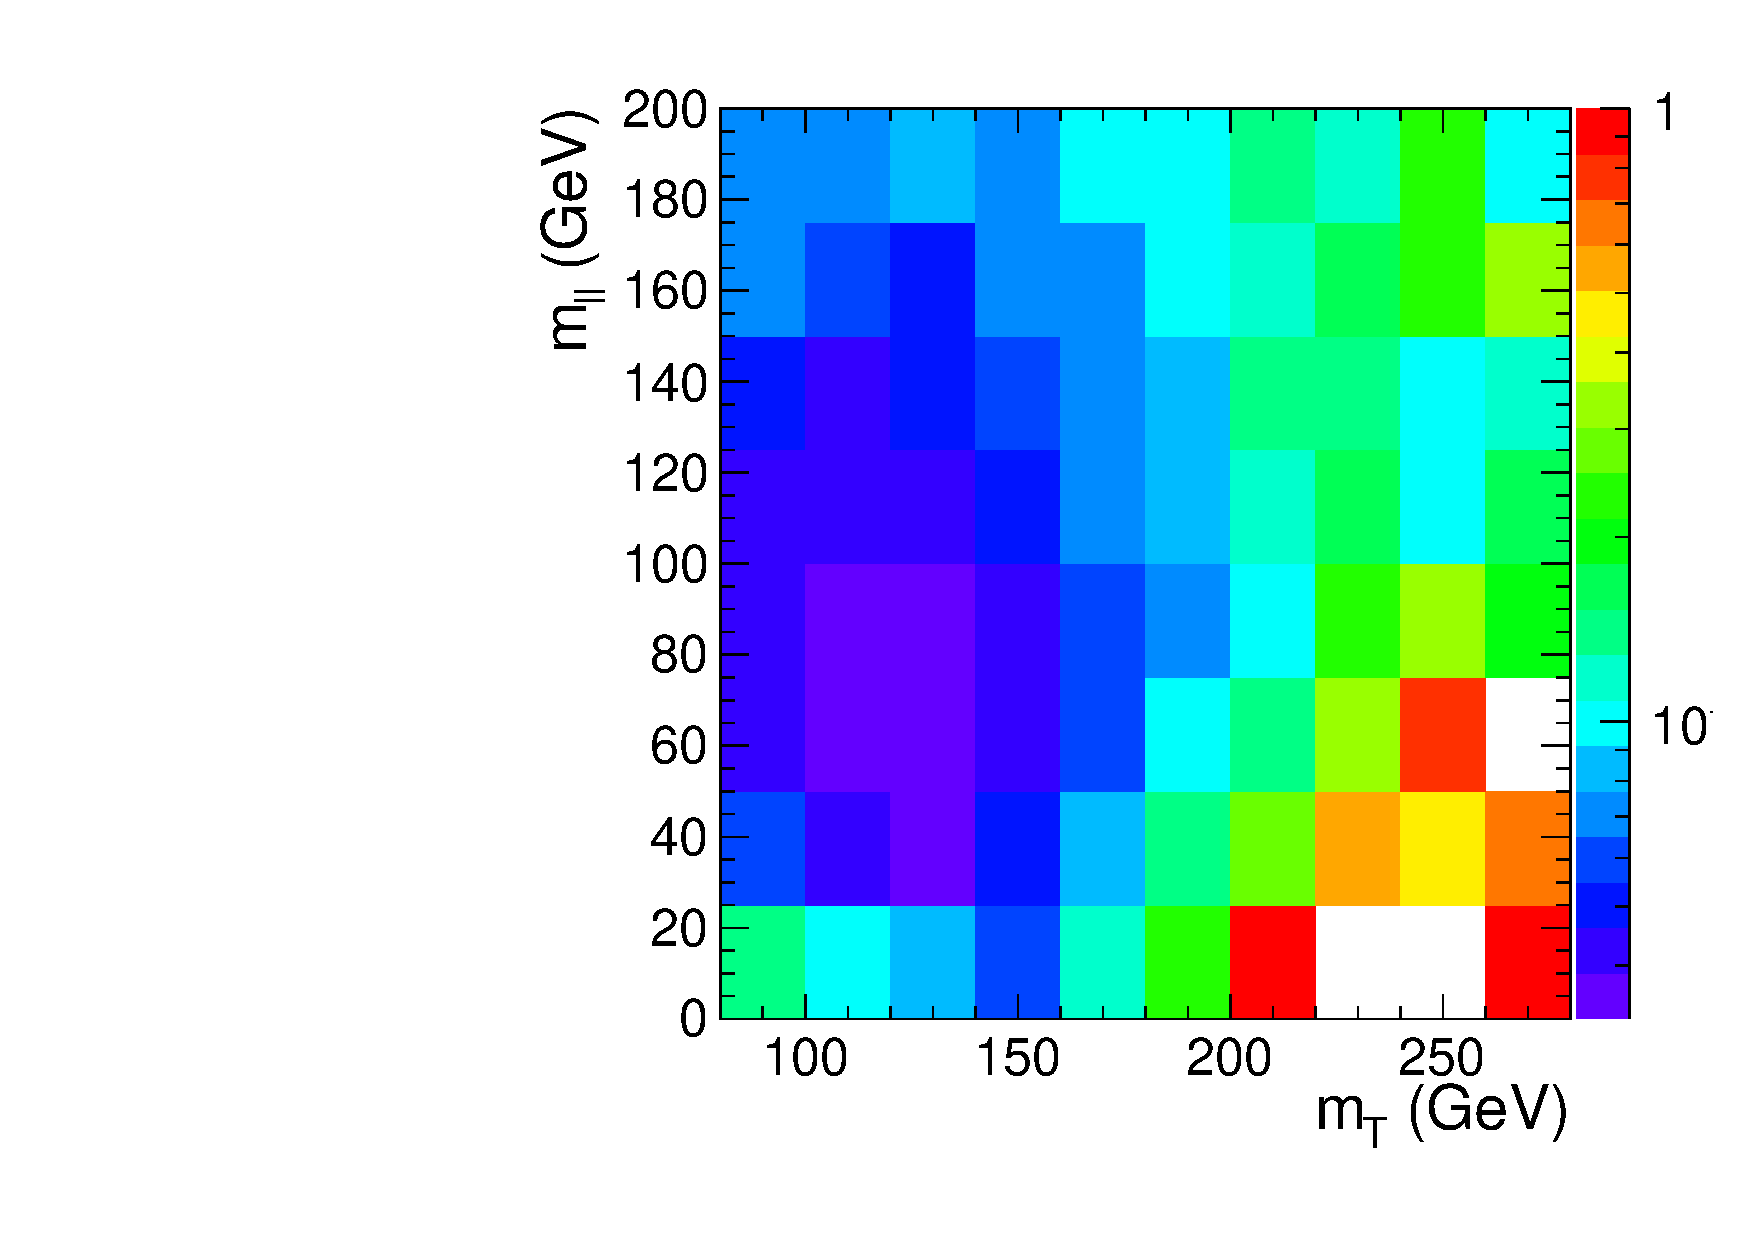
\includegraphics[width=.35\textwidth]{figures/templates/qqWWerr_2D_mH160_0j_of.pdf}
	}

	%
	\centering
	\subfigure[ggWW]{
	\centering
	\label{subfig:template_ggWW_160}
		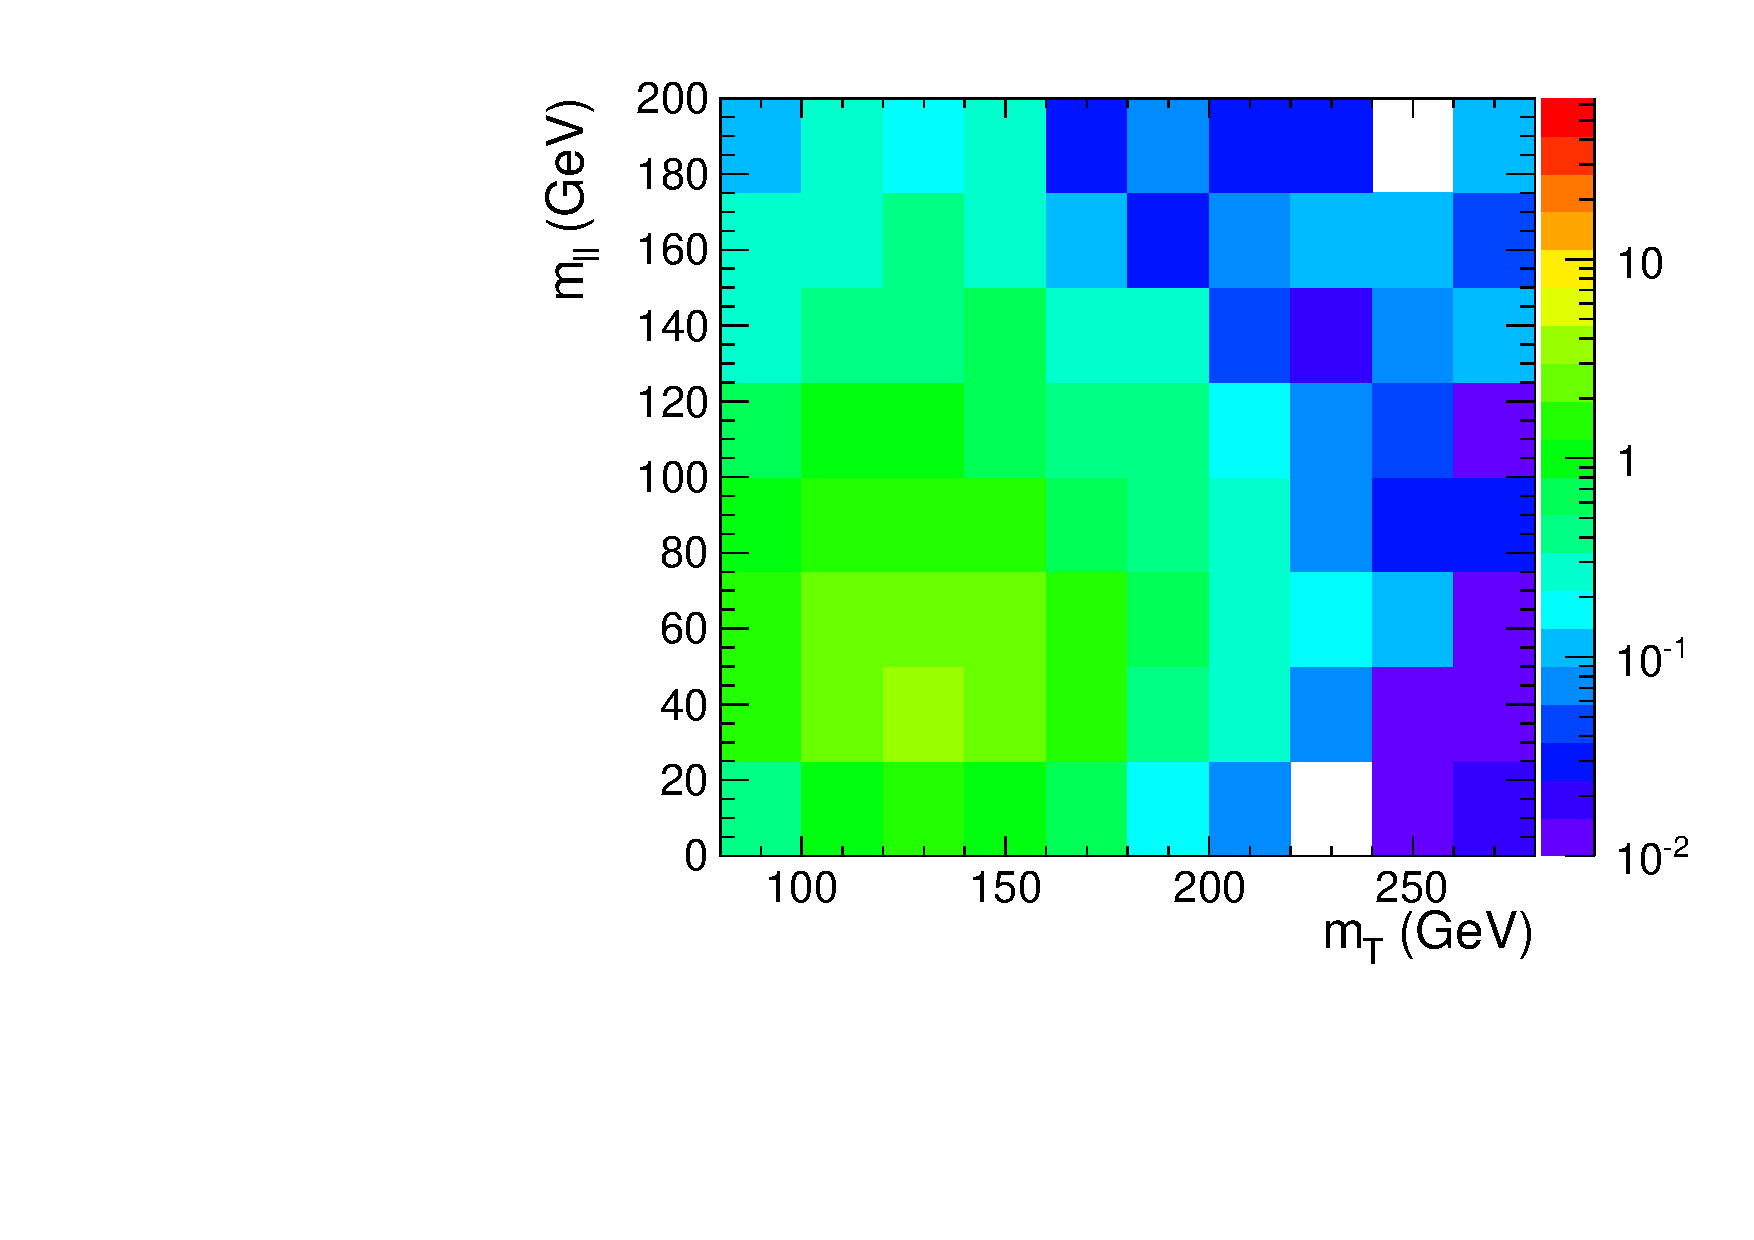
\includegraphics[width=.35\textwidth]{figures/templates/ggWW_2D_mH160_0j_of.pdf}
	}
	\subfigure[ggWW statistical uncertainty]{
	\centering
	\label{subfig:template_ggWWerr_160}
		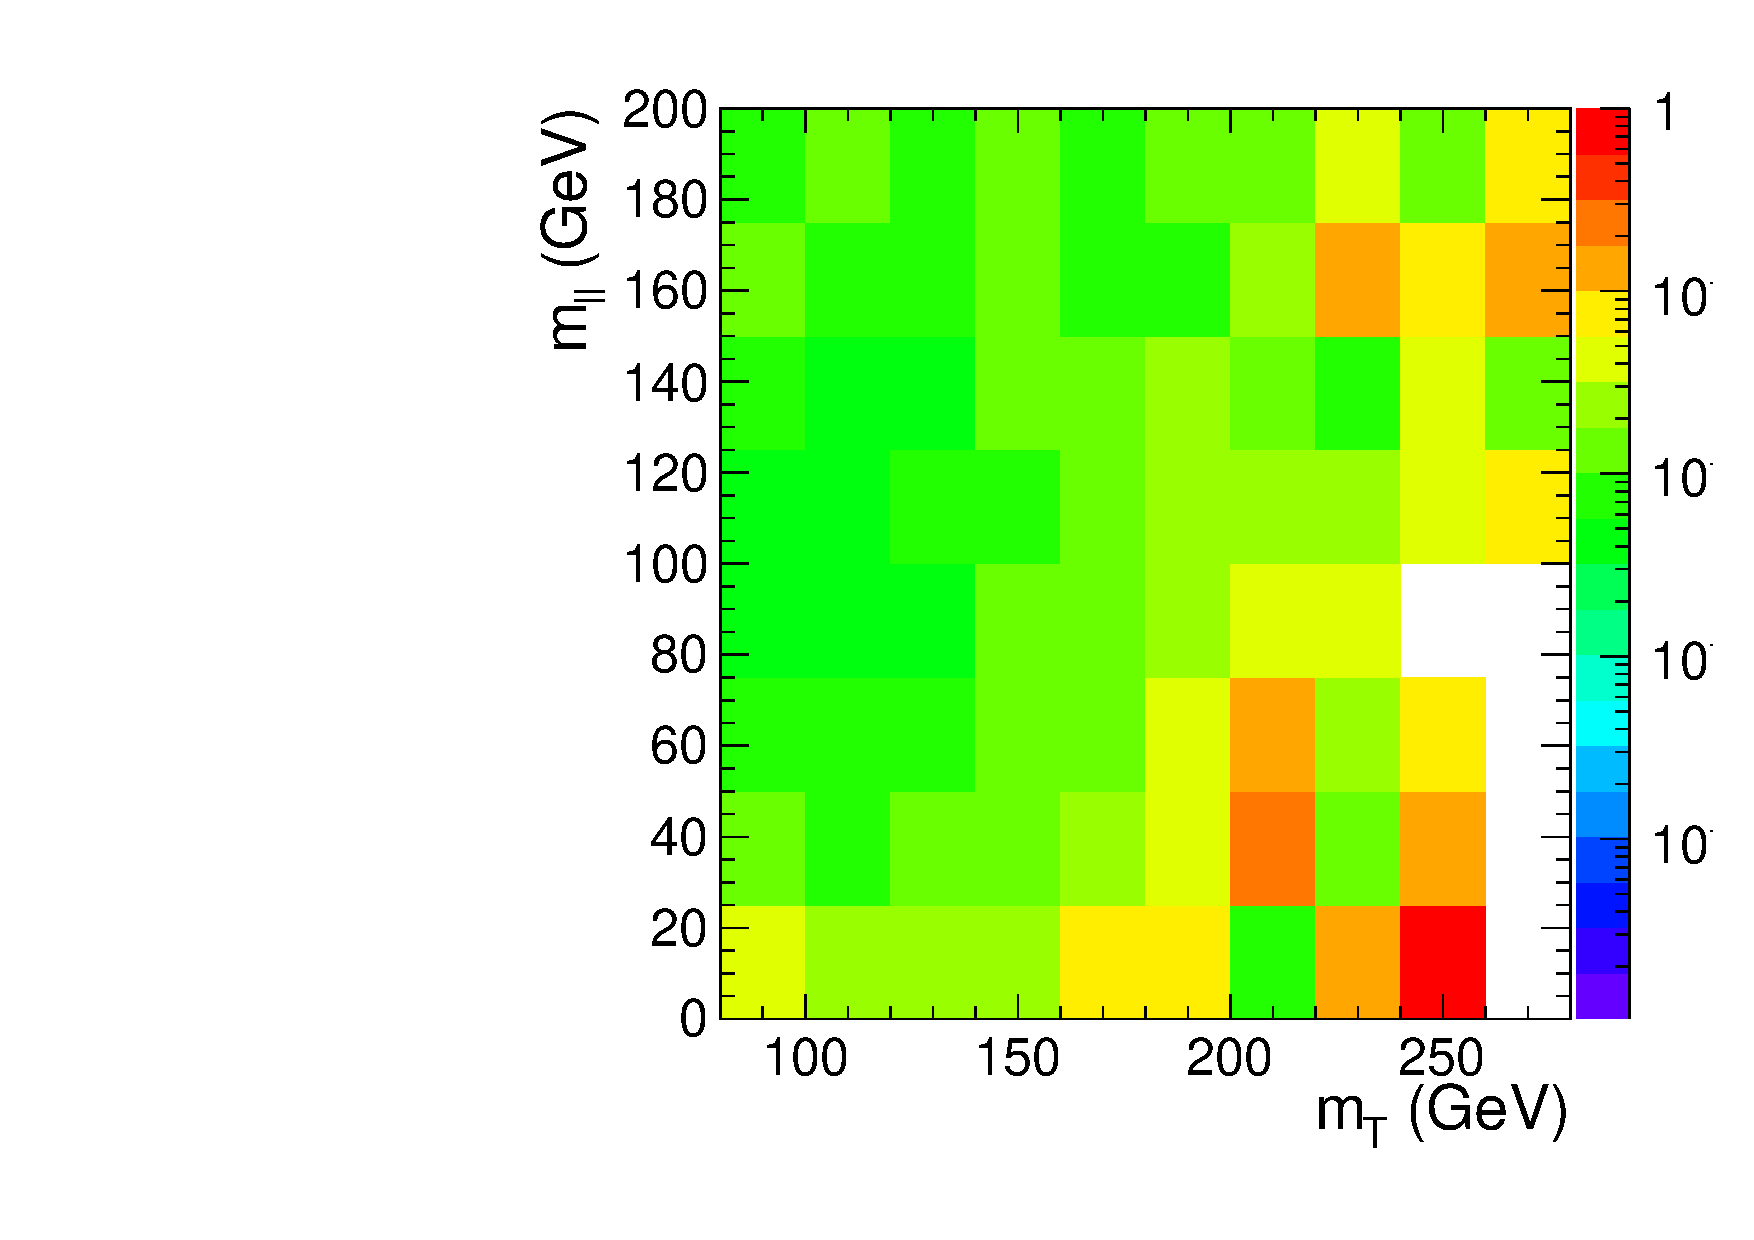
\includegraphics[width=.35\textwidth]{figures/templates/ggWWerr_2D_mH160_0j_of.pdf}
	}

	\caption{2D templates at \mHi = 160 \GeV} 
	\label{fig:templates_160_1}

\end{figure}

\begin{figure}[!hbtp]
	
	%
	\centering
	\subfigure[Wjets]{
	\centering
	\label{subfig:template_Wjets_160}
		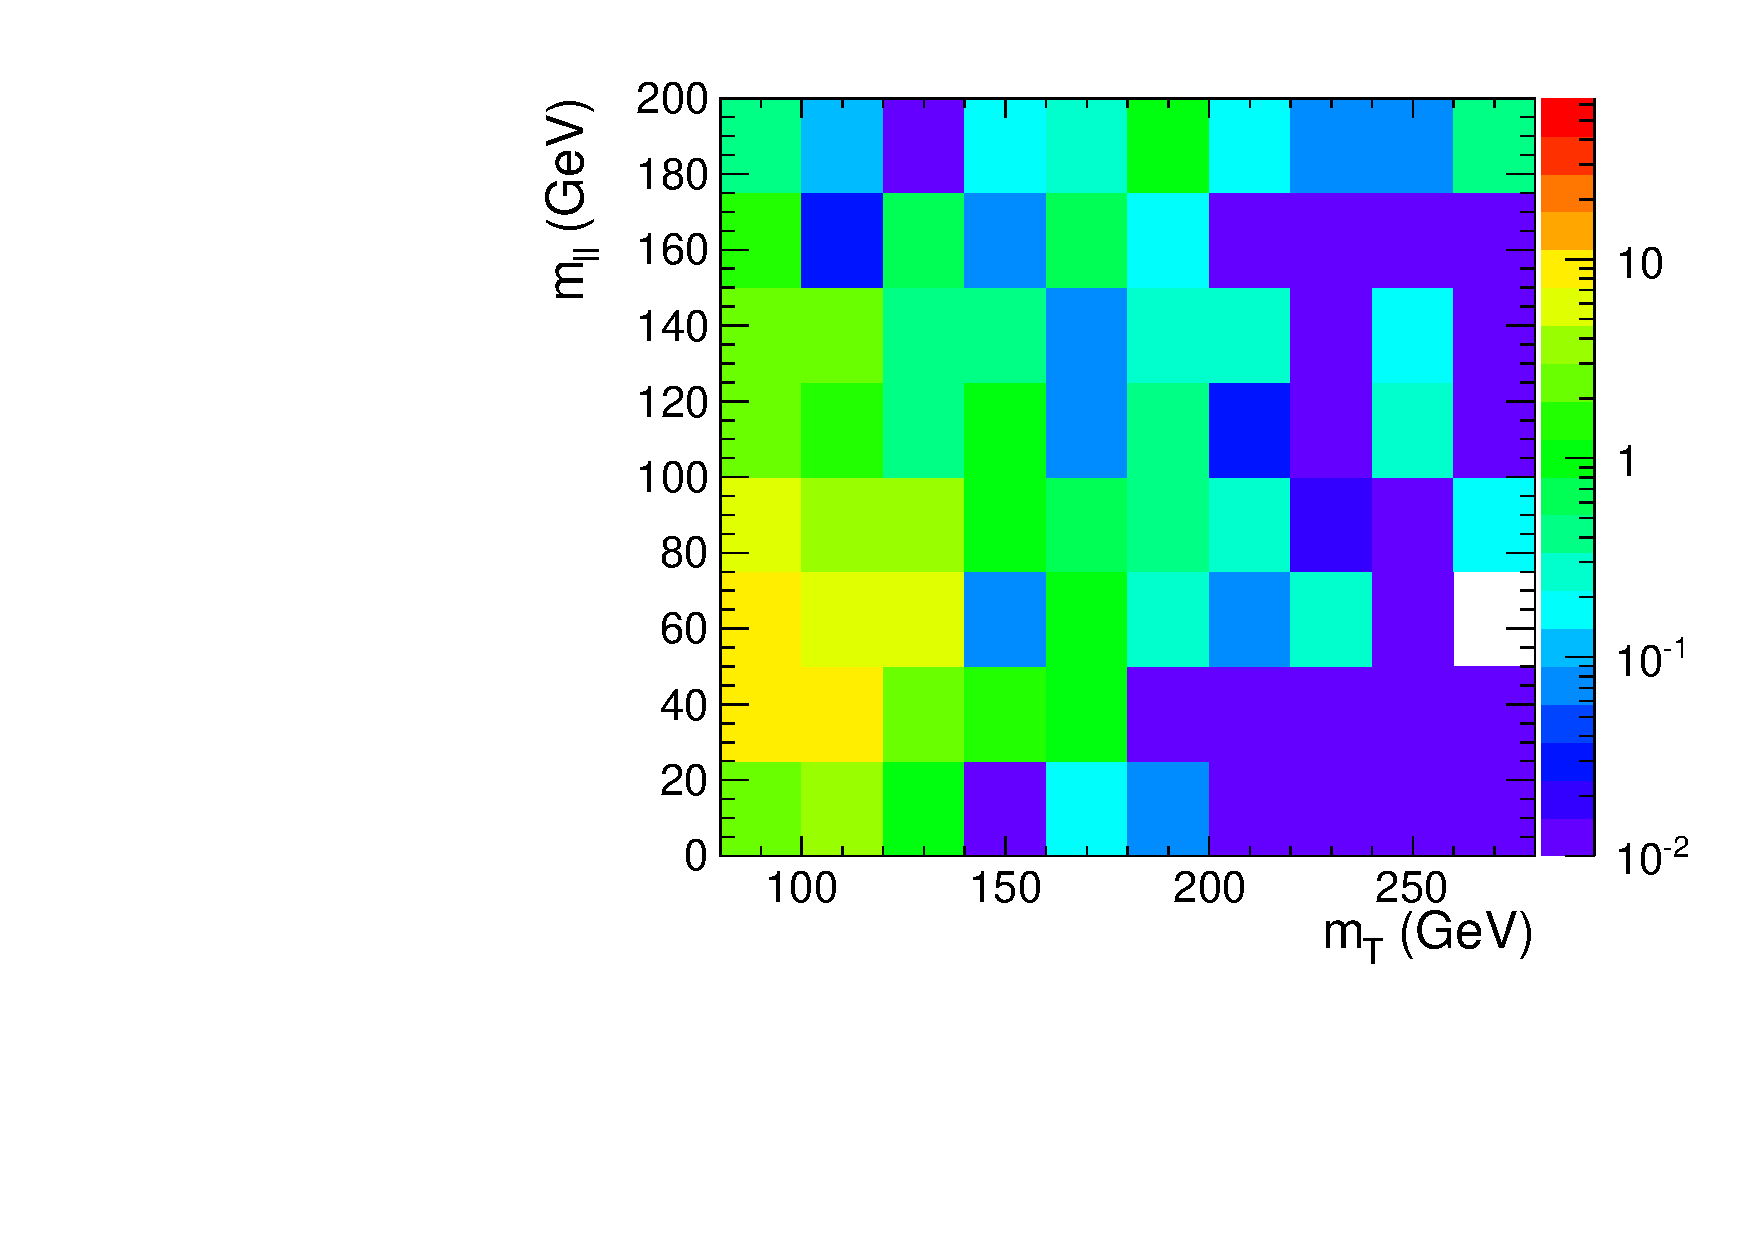
\includegraphics[width=.35\textwidth]{figures/templates/Wjets_2D_mH160_0j_of.pdf}
	}
	\subfigure[Wjets statistical uncertainty]{
	\centering
	\label{subfig:template_Wjetserr_160}
		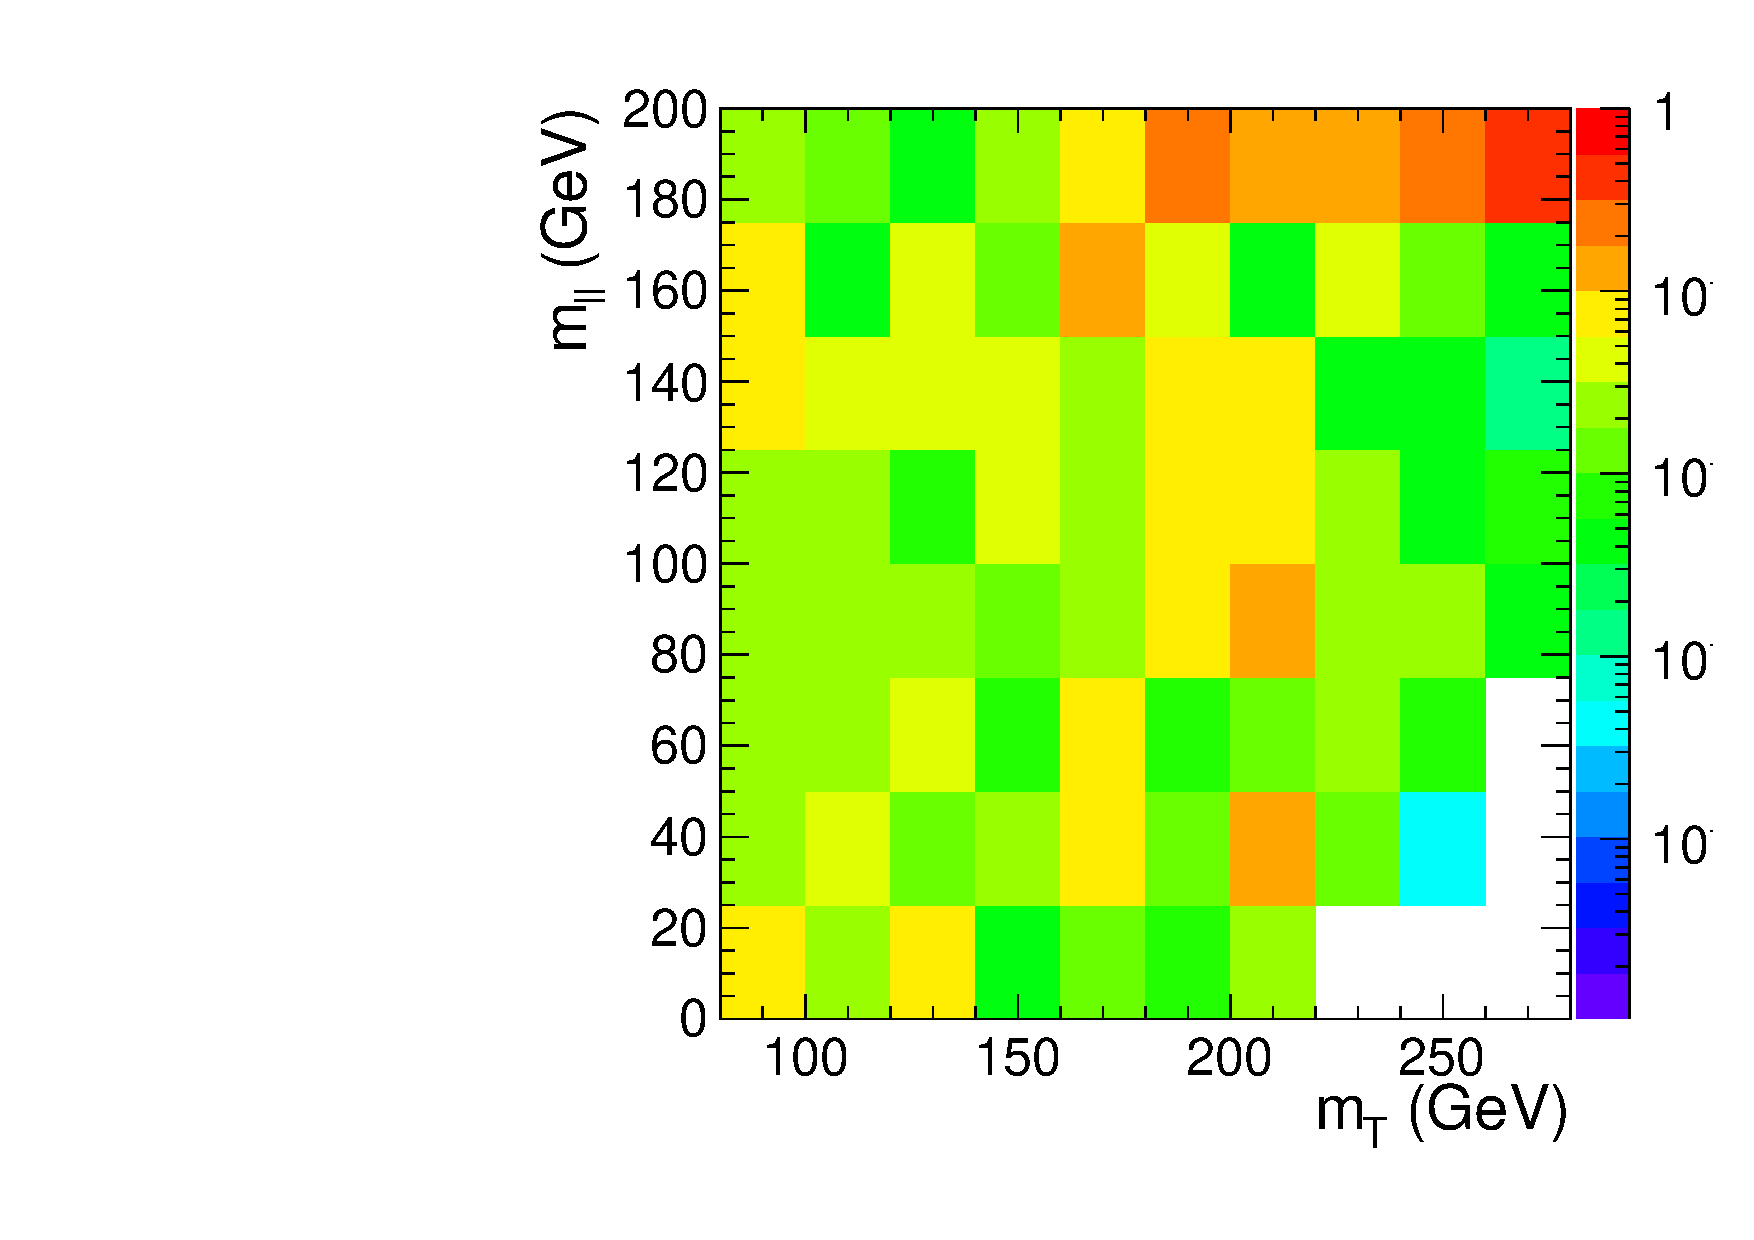
\includegraphics[width=.35\textwidth]{figures/templates/Wjetserr_2D_mH160_0j_of.pdf}
	}
	
	%
	\centering
	\subfigure[Top]{
	\centering
	\label{subfig:template_Top_160}
		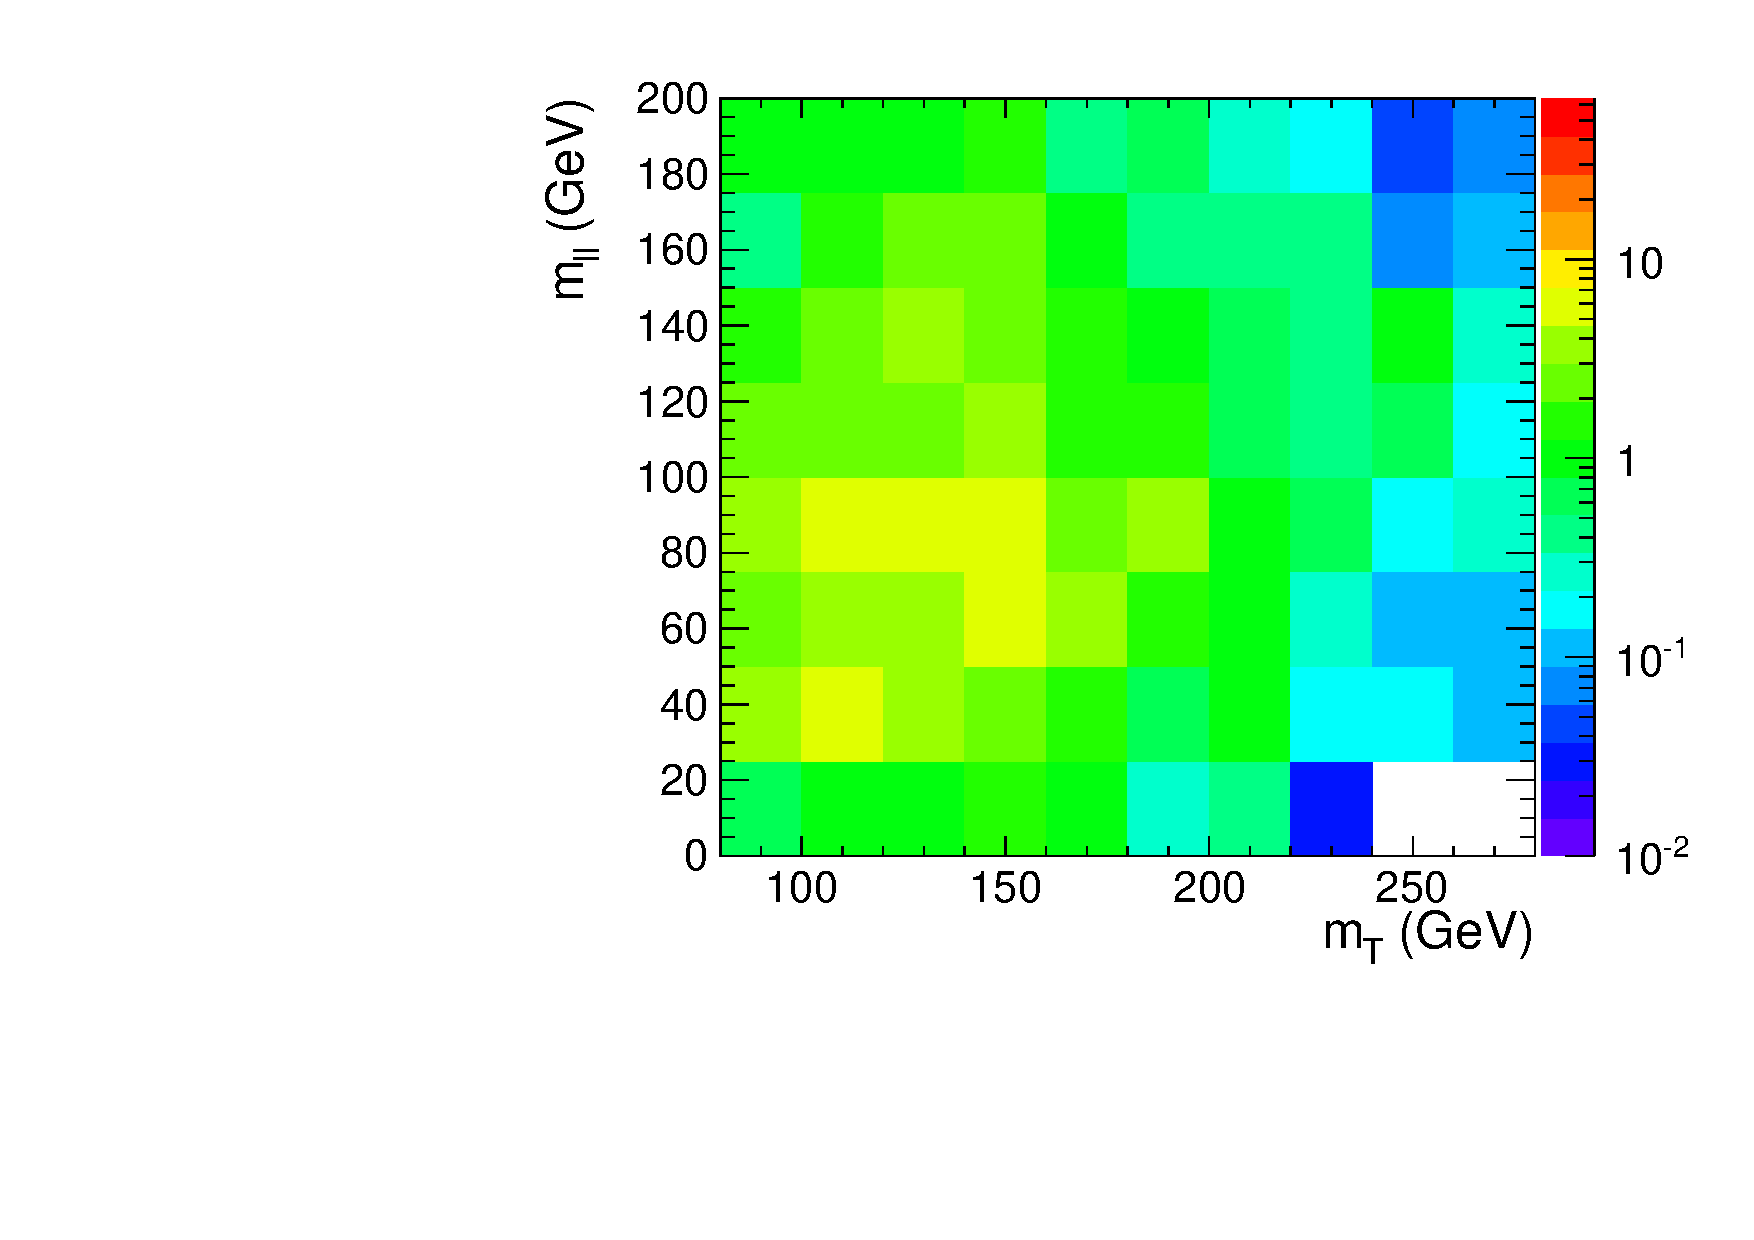
\includegraphics[width=.35\textwidth]{figures/templates/Top_2D_mH160_0j_of.pdf}
	}
	\subfigure[Top statistical uncertainty]{
	\centering
	\label{subfig:template_Toperr_160}
		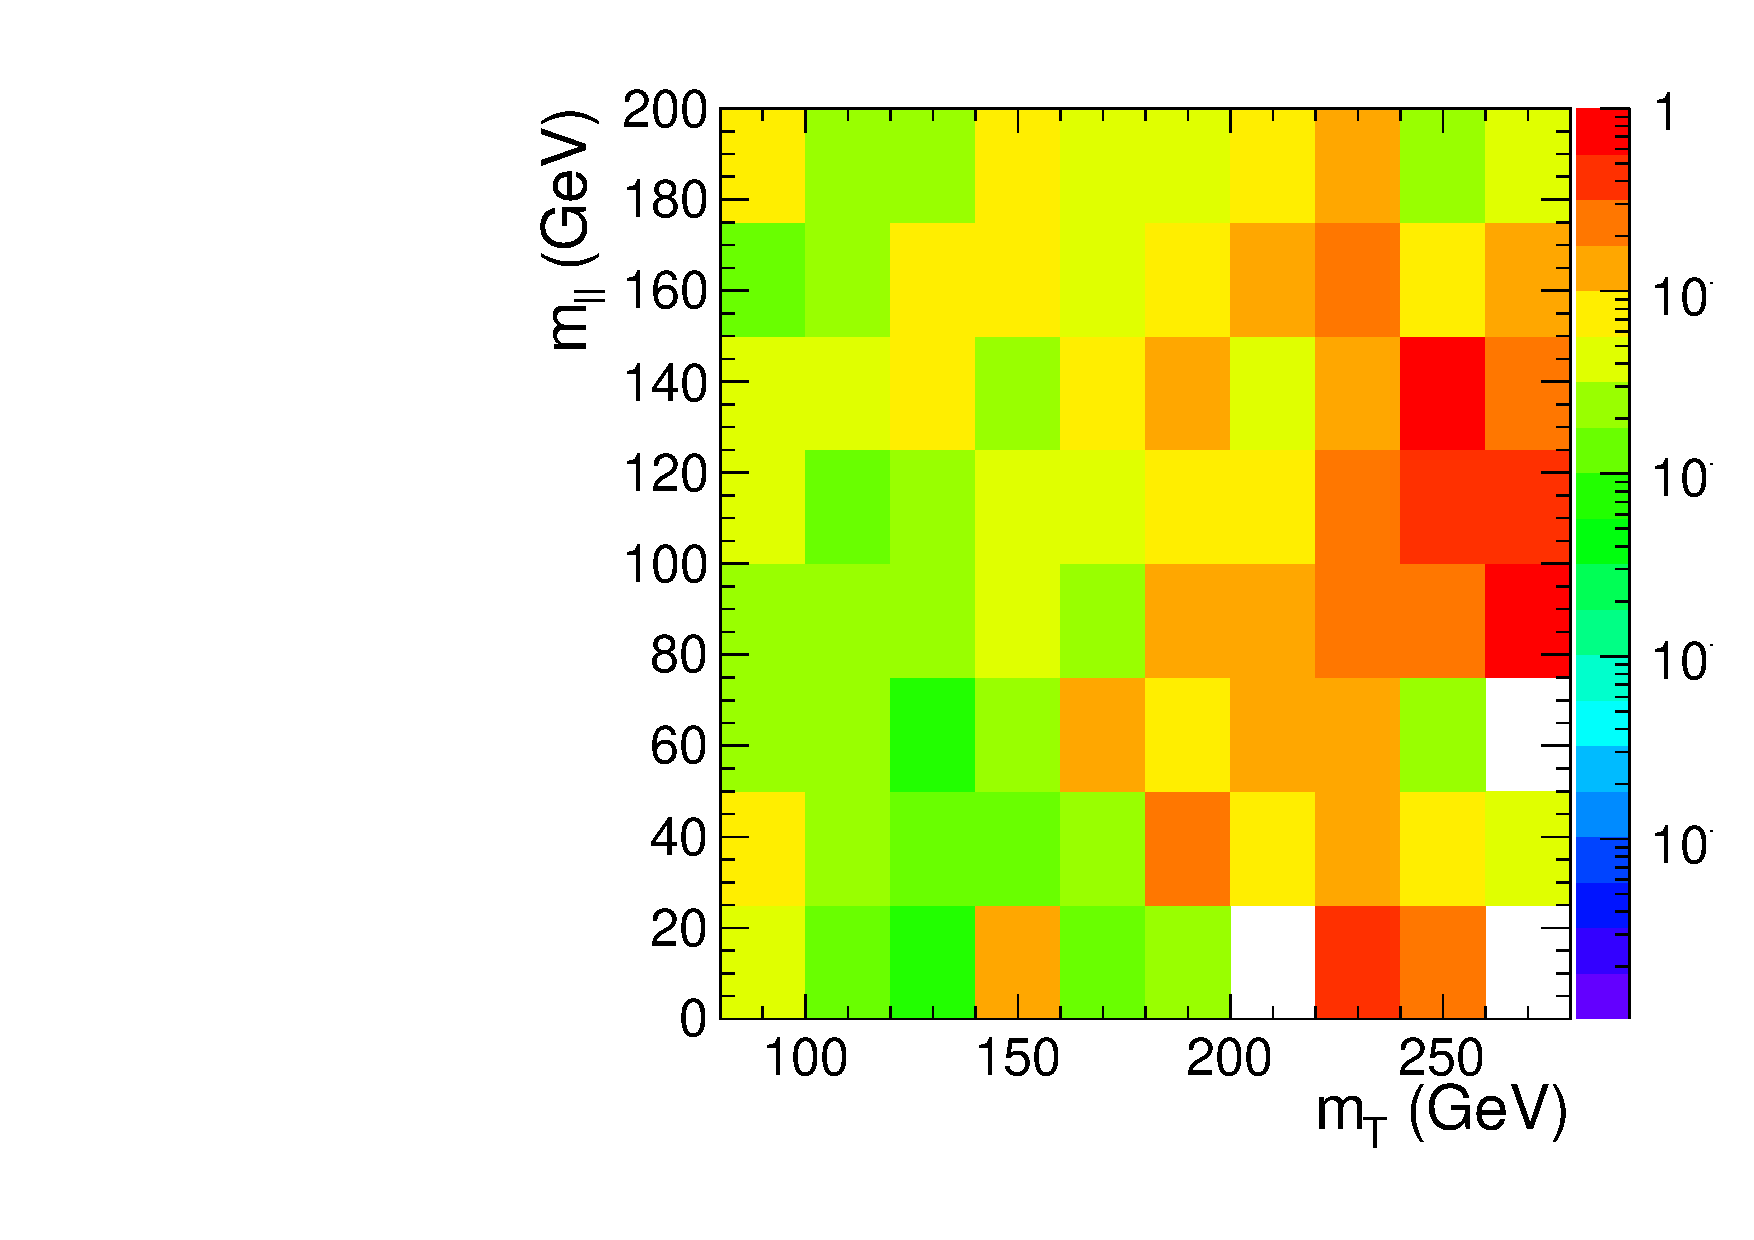
\includegraphics[width=.35\textwidth]{figures/templates/Toperr_2D_mH160_0j_of.pdf}
	}

	%
	\centering
	\subfigure[VV]{
	\centering
	\label{subfig:template_VV_160}
		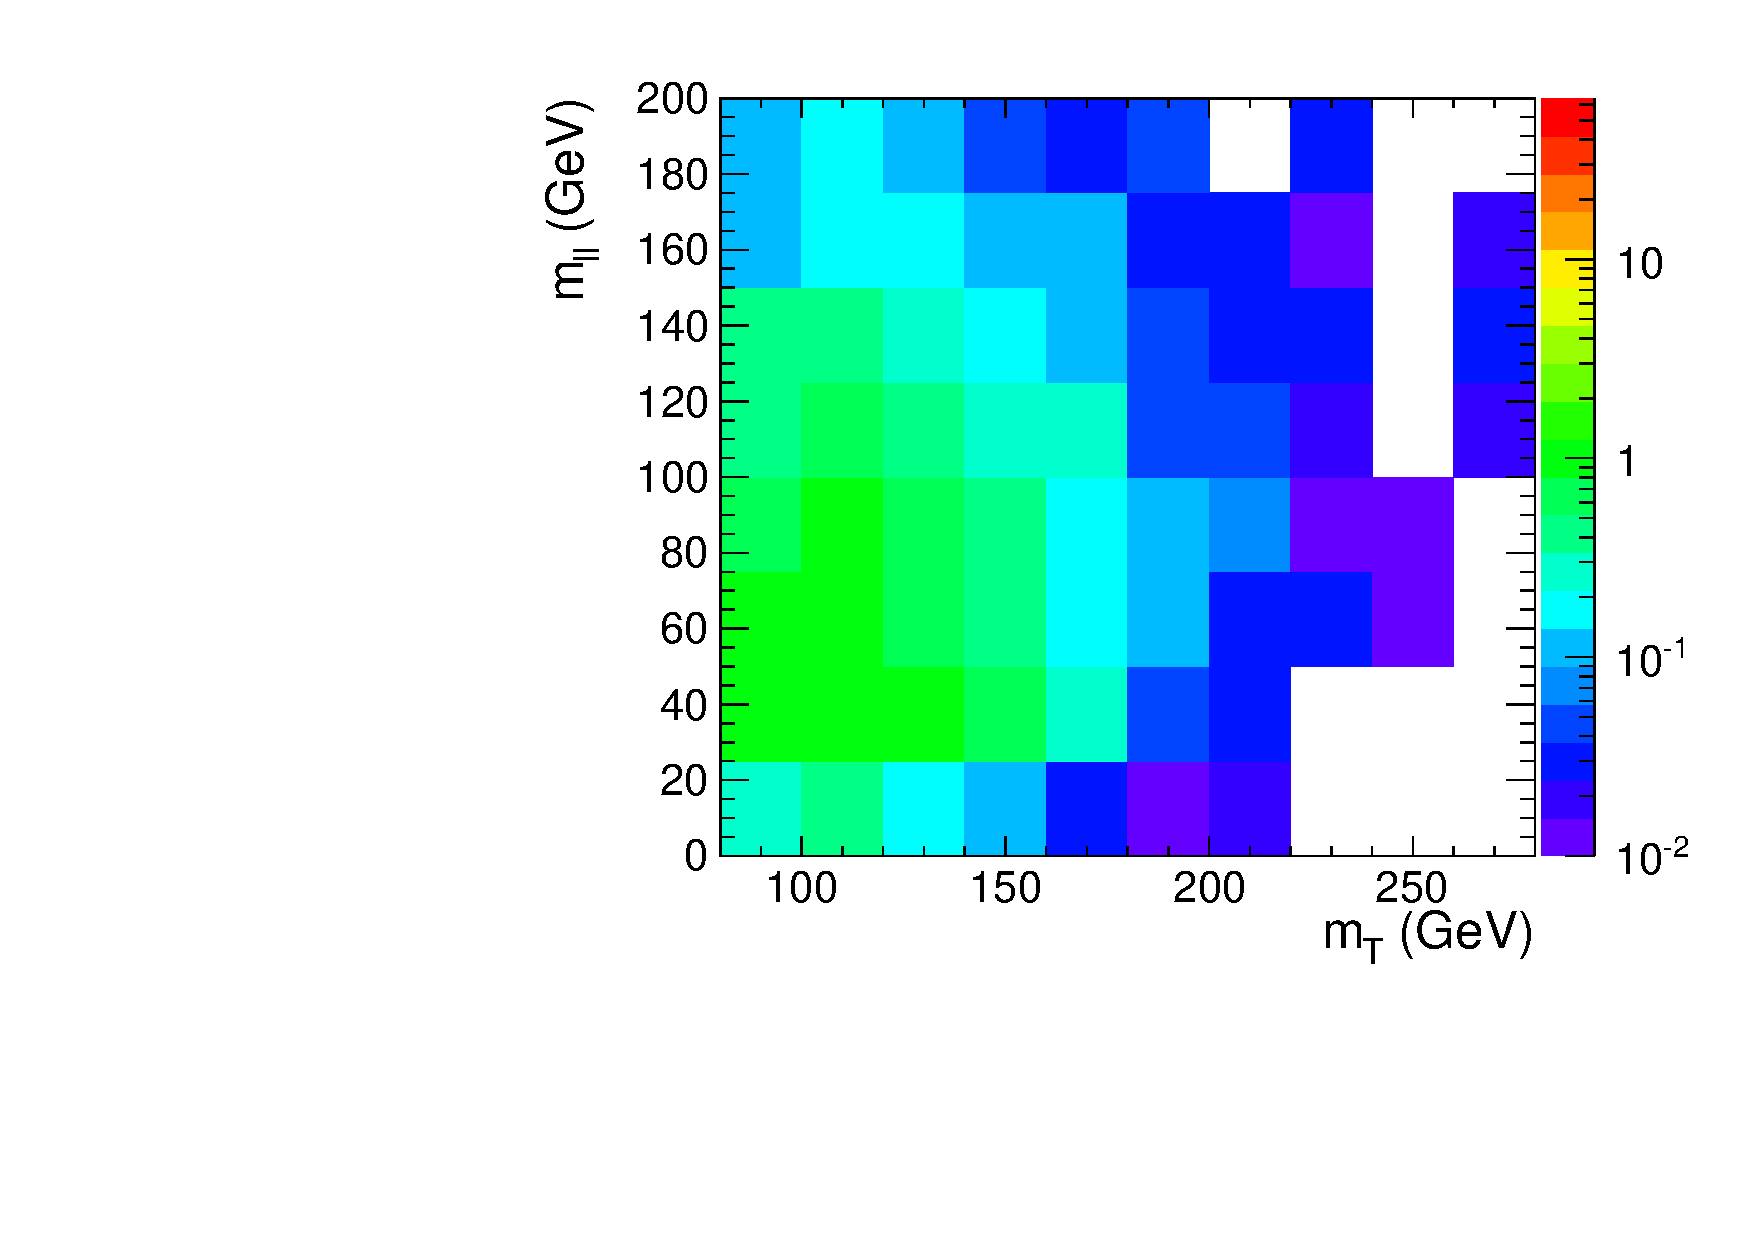
\includegraphics[width=.35\textwidth]{figures/templates/VV_2D_mH160_0j_of.pdf}
	}
	\subfigure[VV statistical uncertainty]{
	\centering
	\label{subfig:template_VVerr_160}
		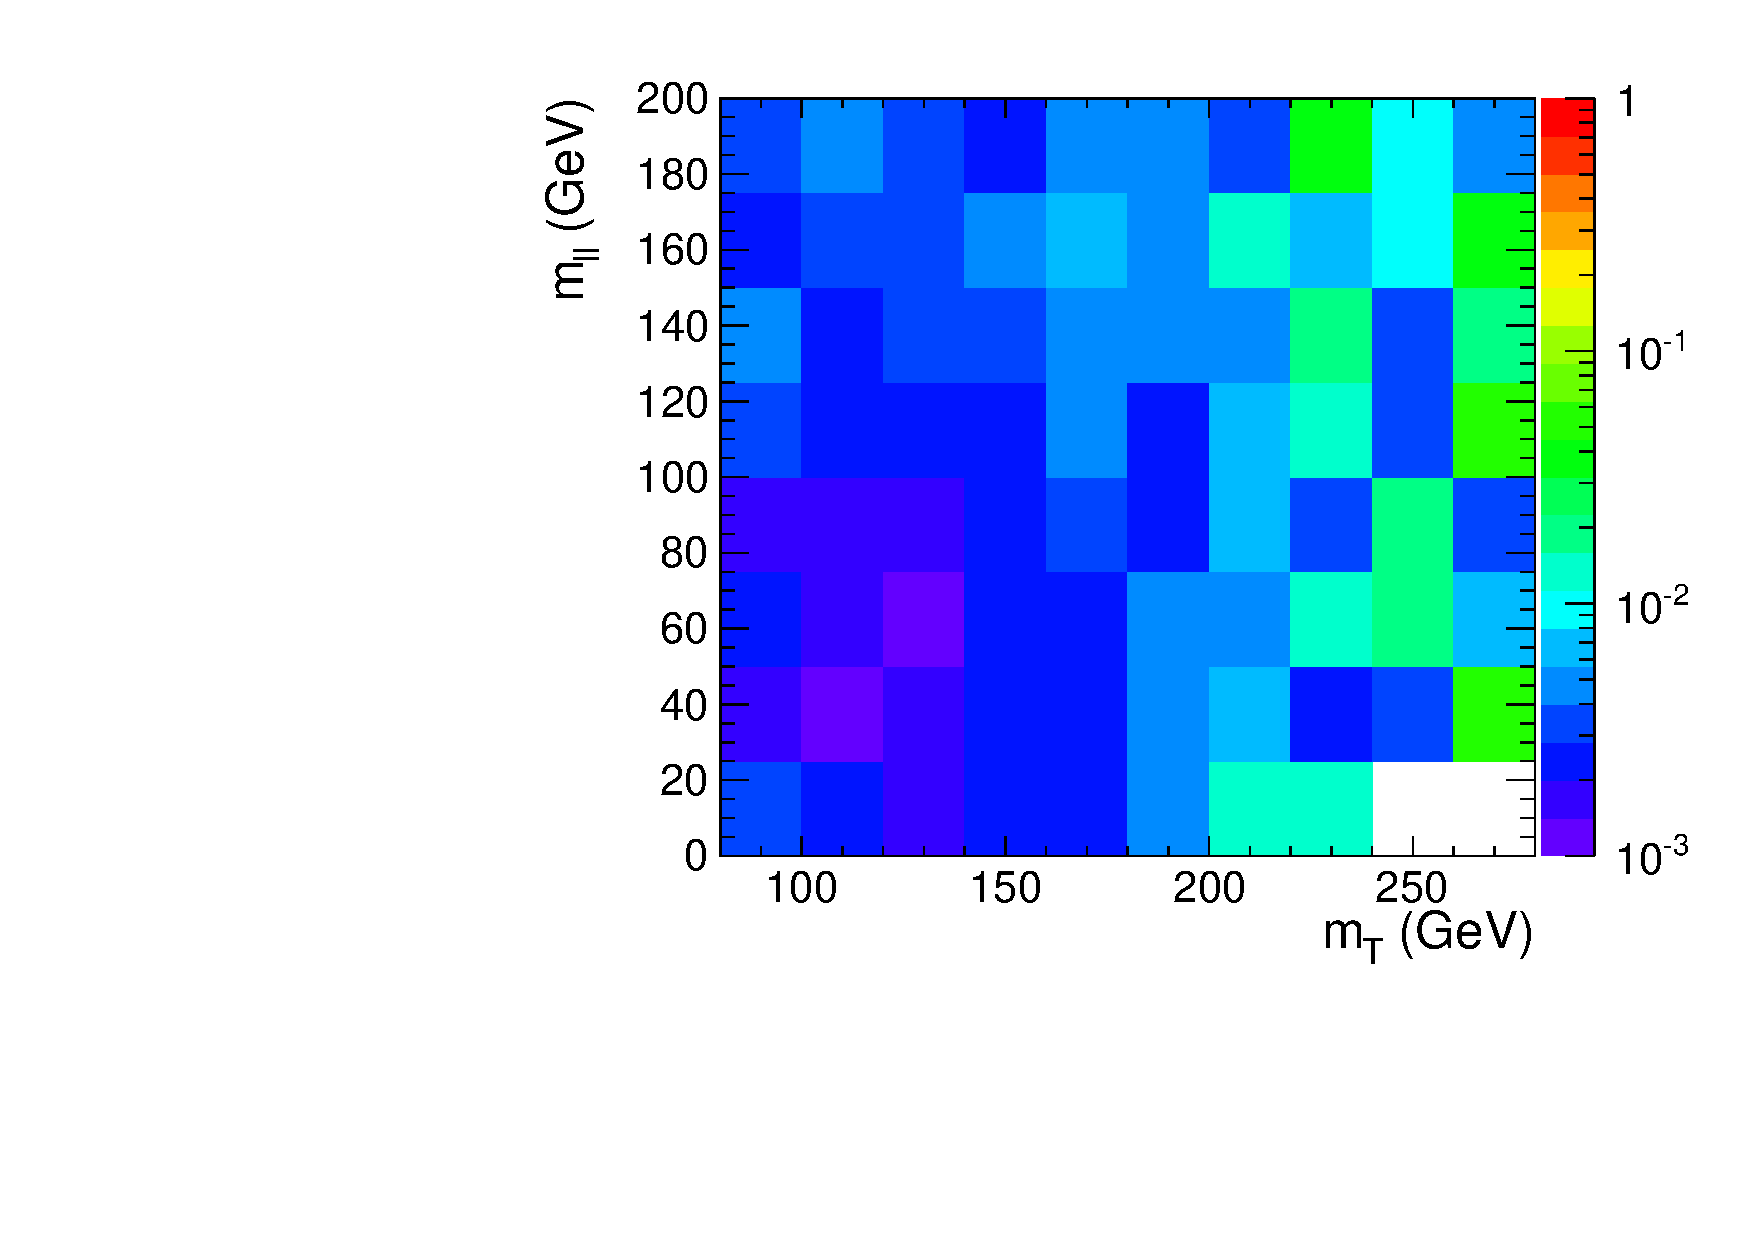
\includegraphics[width=.35\textwidth]{figures/templates/VVerr_2D_mH160_0j_of.pdf}
	}

	\caption{2D templates at \mHi = 160 \GeV} 
	\label{fig:templates_160_2}

\end{figure}

\begin{figure}[!hbtp]
	
	%
	\centering
	\subfigure[Zjets]{
	\centering
	\label{subfig:template_Zjets_160}
		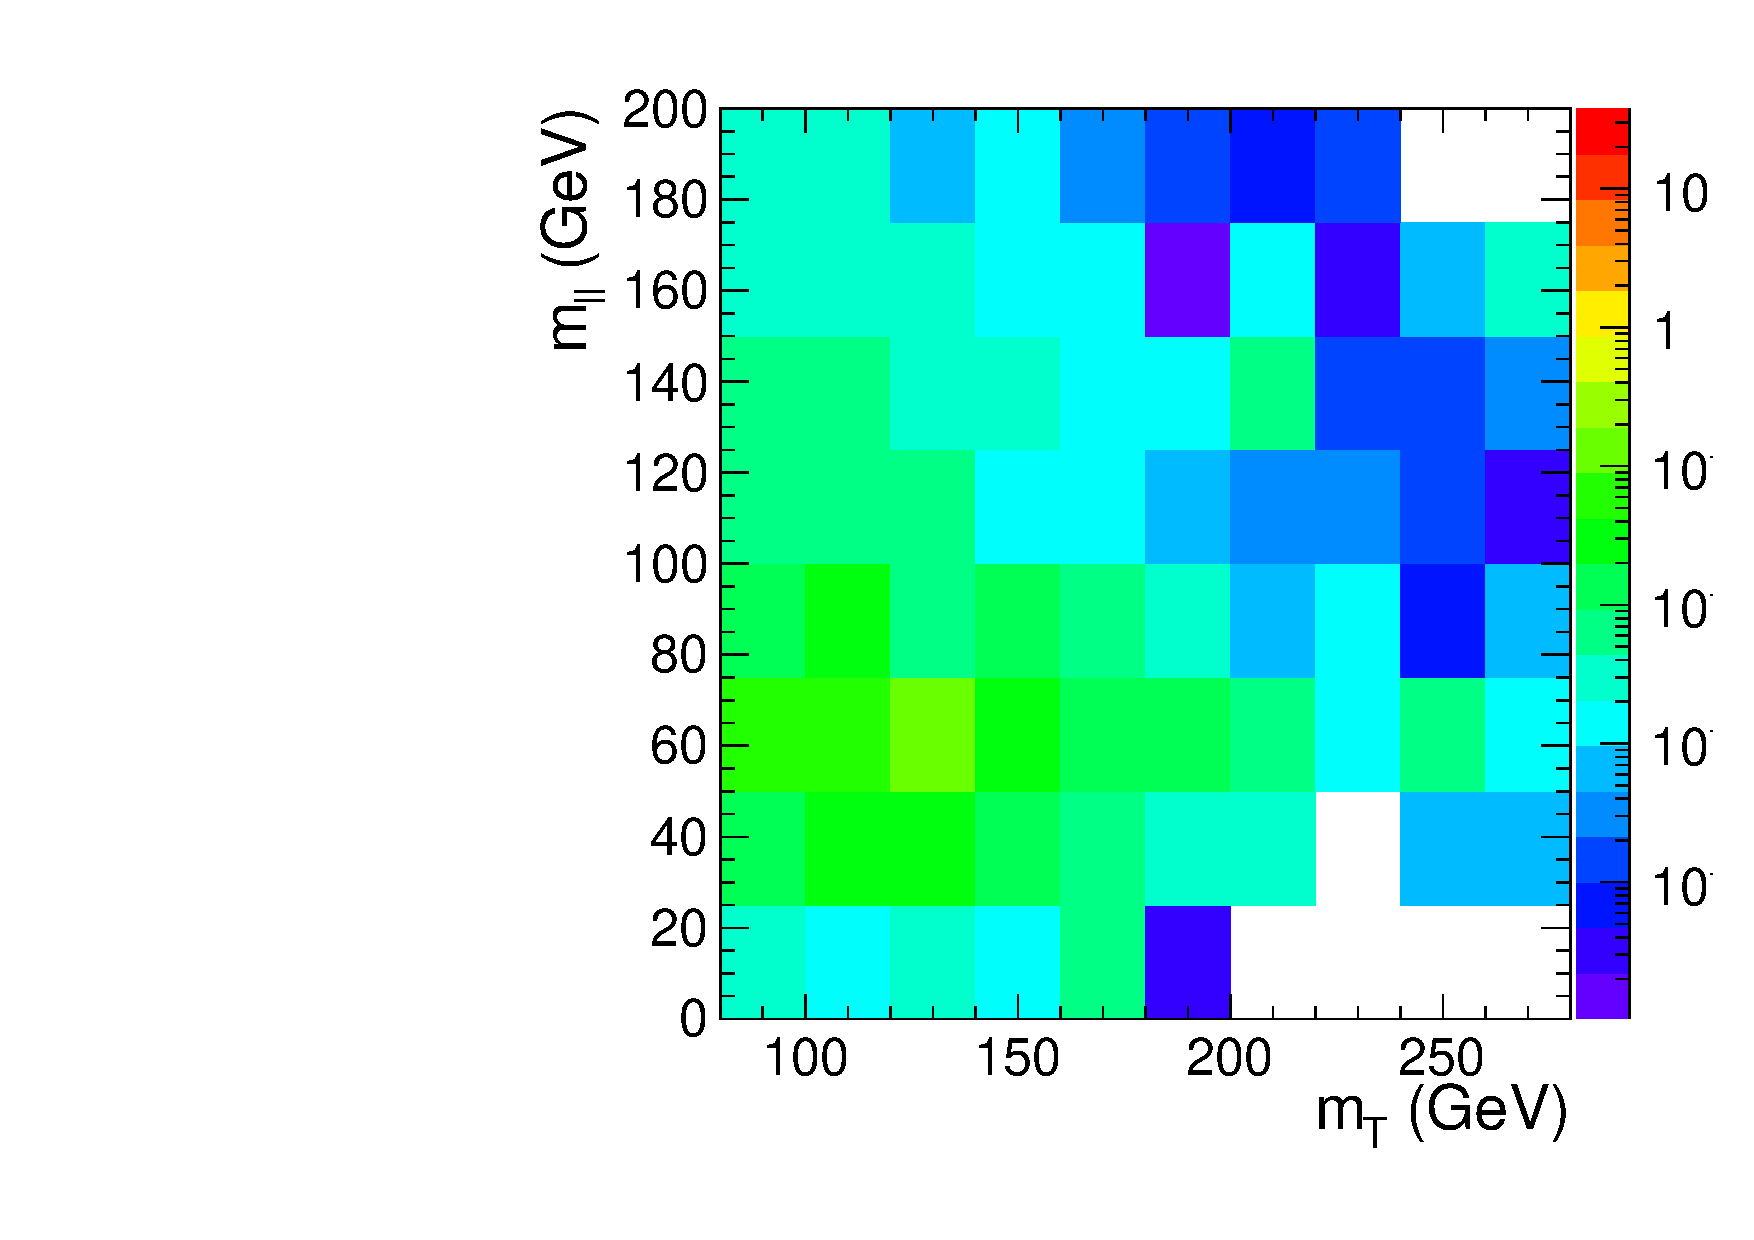
\includegraphics[width=.35\textwidth]{figures/templates/Zjets_2D_mH160_0j_of.pdf}
	}
	\subfigure[Zjets statistical uncertainty]{
	\centering
	\label{subfig:template_Zjetserr_160}
		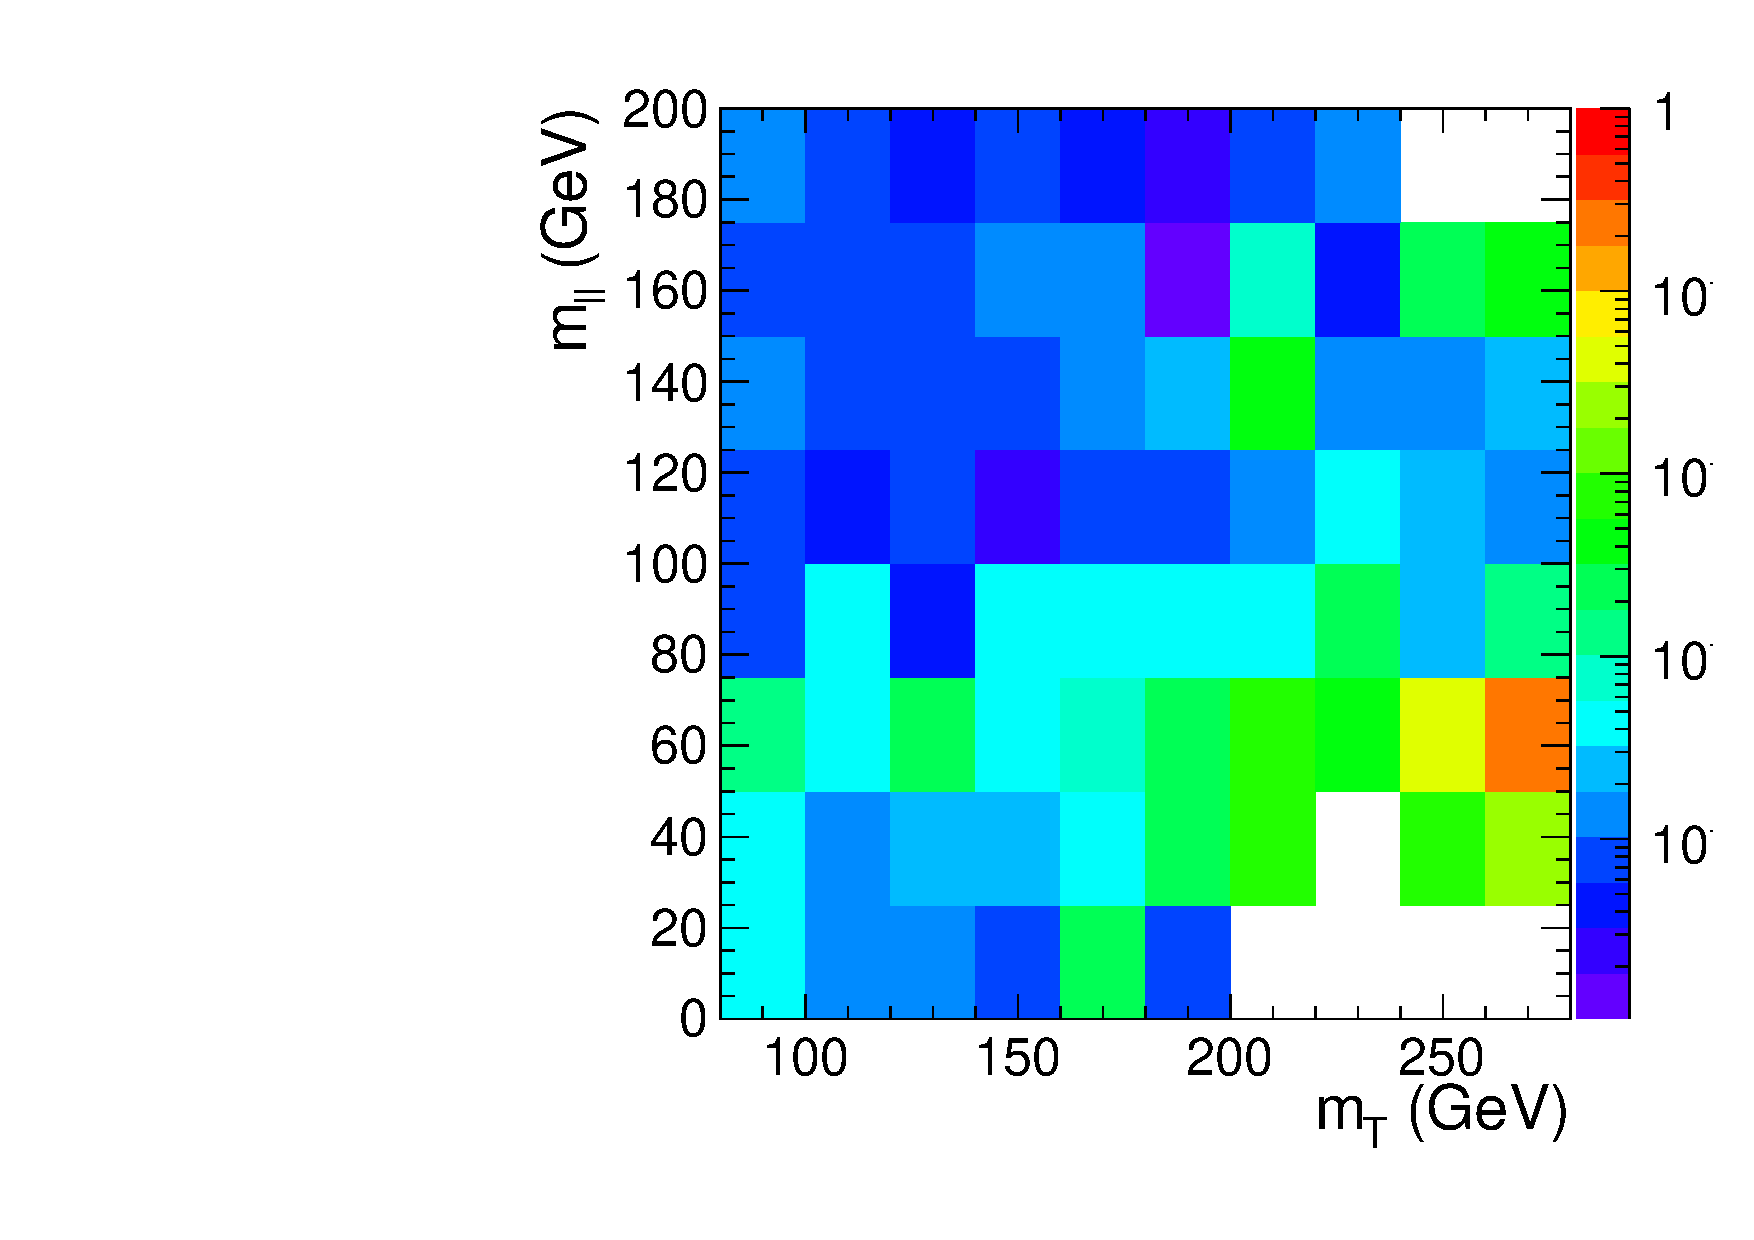
\includegraphics[width=.35\textwidth]{figures/templates/Zjetserr_2D_mH160_0j_of.pdf}
	}

	%
	\centering
	\subfigure[Wgamma]{
	\centering
	\label{subfig:template_Wgamma_160}
		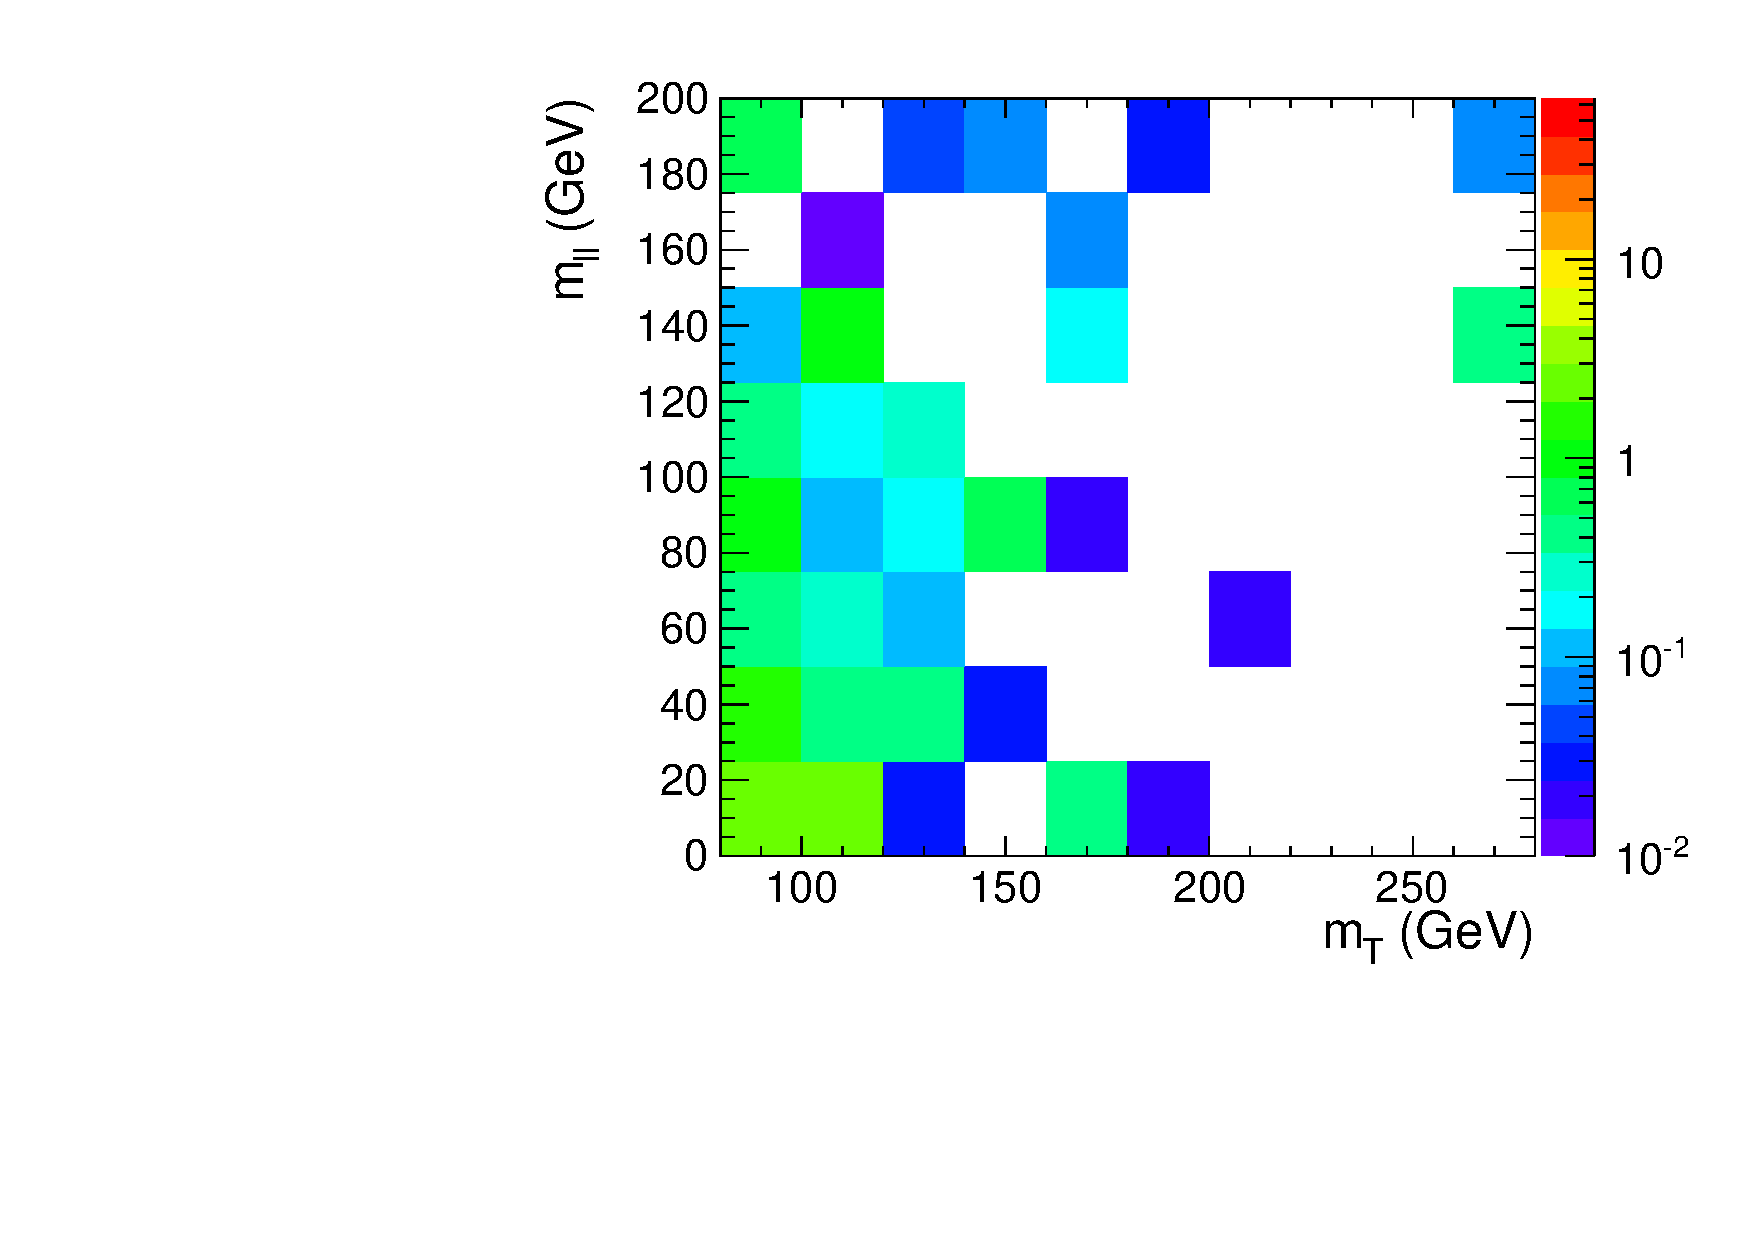
\includegraphics[width=.35\textwidth]{figures/templates/Wgamma_2D_mH160_0j_of.pdf}
	}
	\subfigure[Wgamma statistical uncertainty]{
	\centering
	\label{subfig:template_Wgammaerr_160}
		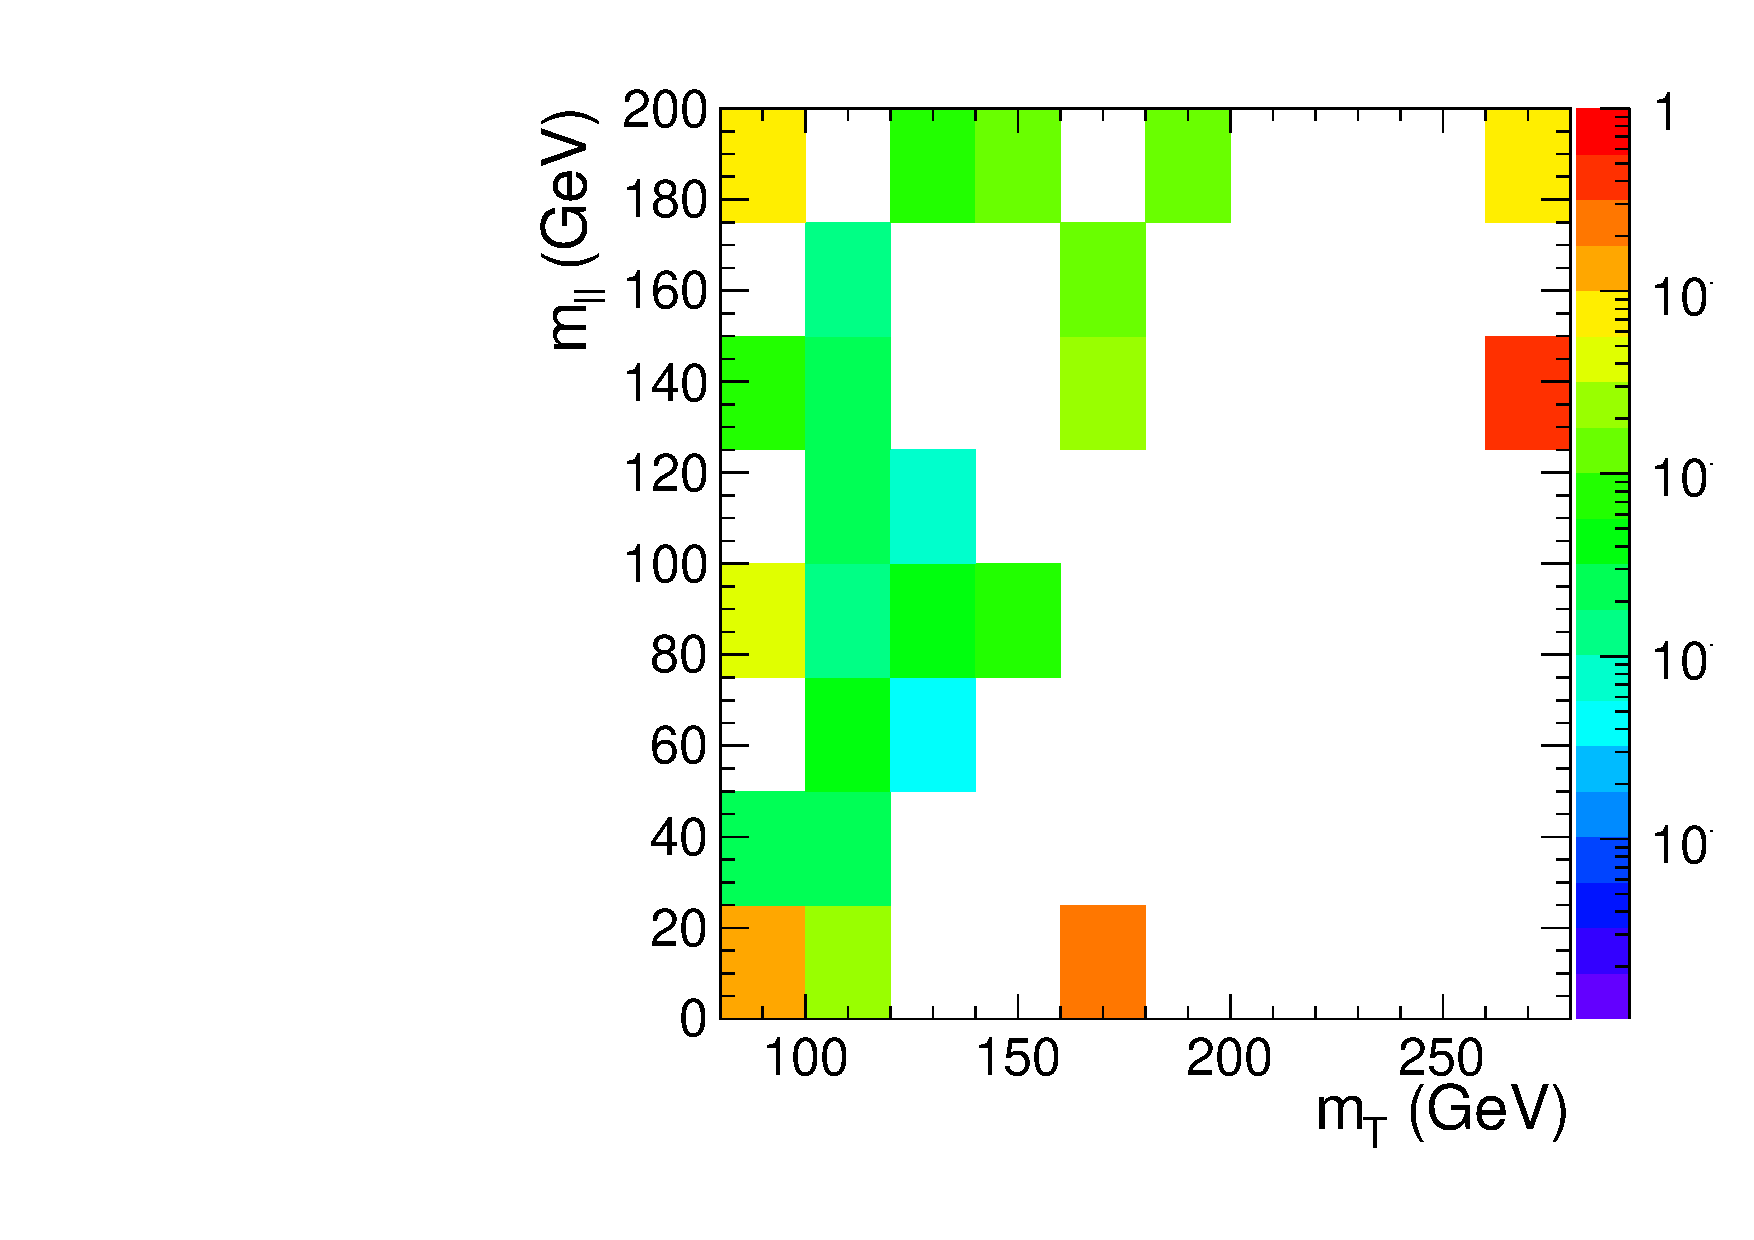
\includegraphics[width=.35\textwidth]{figures/templates/Wgammaerr_2D_mH160_0j_of.pdf}
	}

	\caption{2D templates at \mHi = 160 \GeV} 
	\label{fig:templates_160_3}

\end{figure} 

\begin{figure}[!hbtp]
	
	%
	\centering
	\subfigure[Stacked unrolled template linear]{
	\centering
	\label{subfig:template_unroll_stack_lin}
		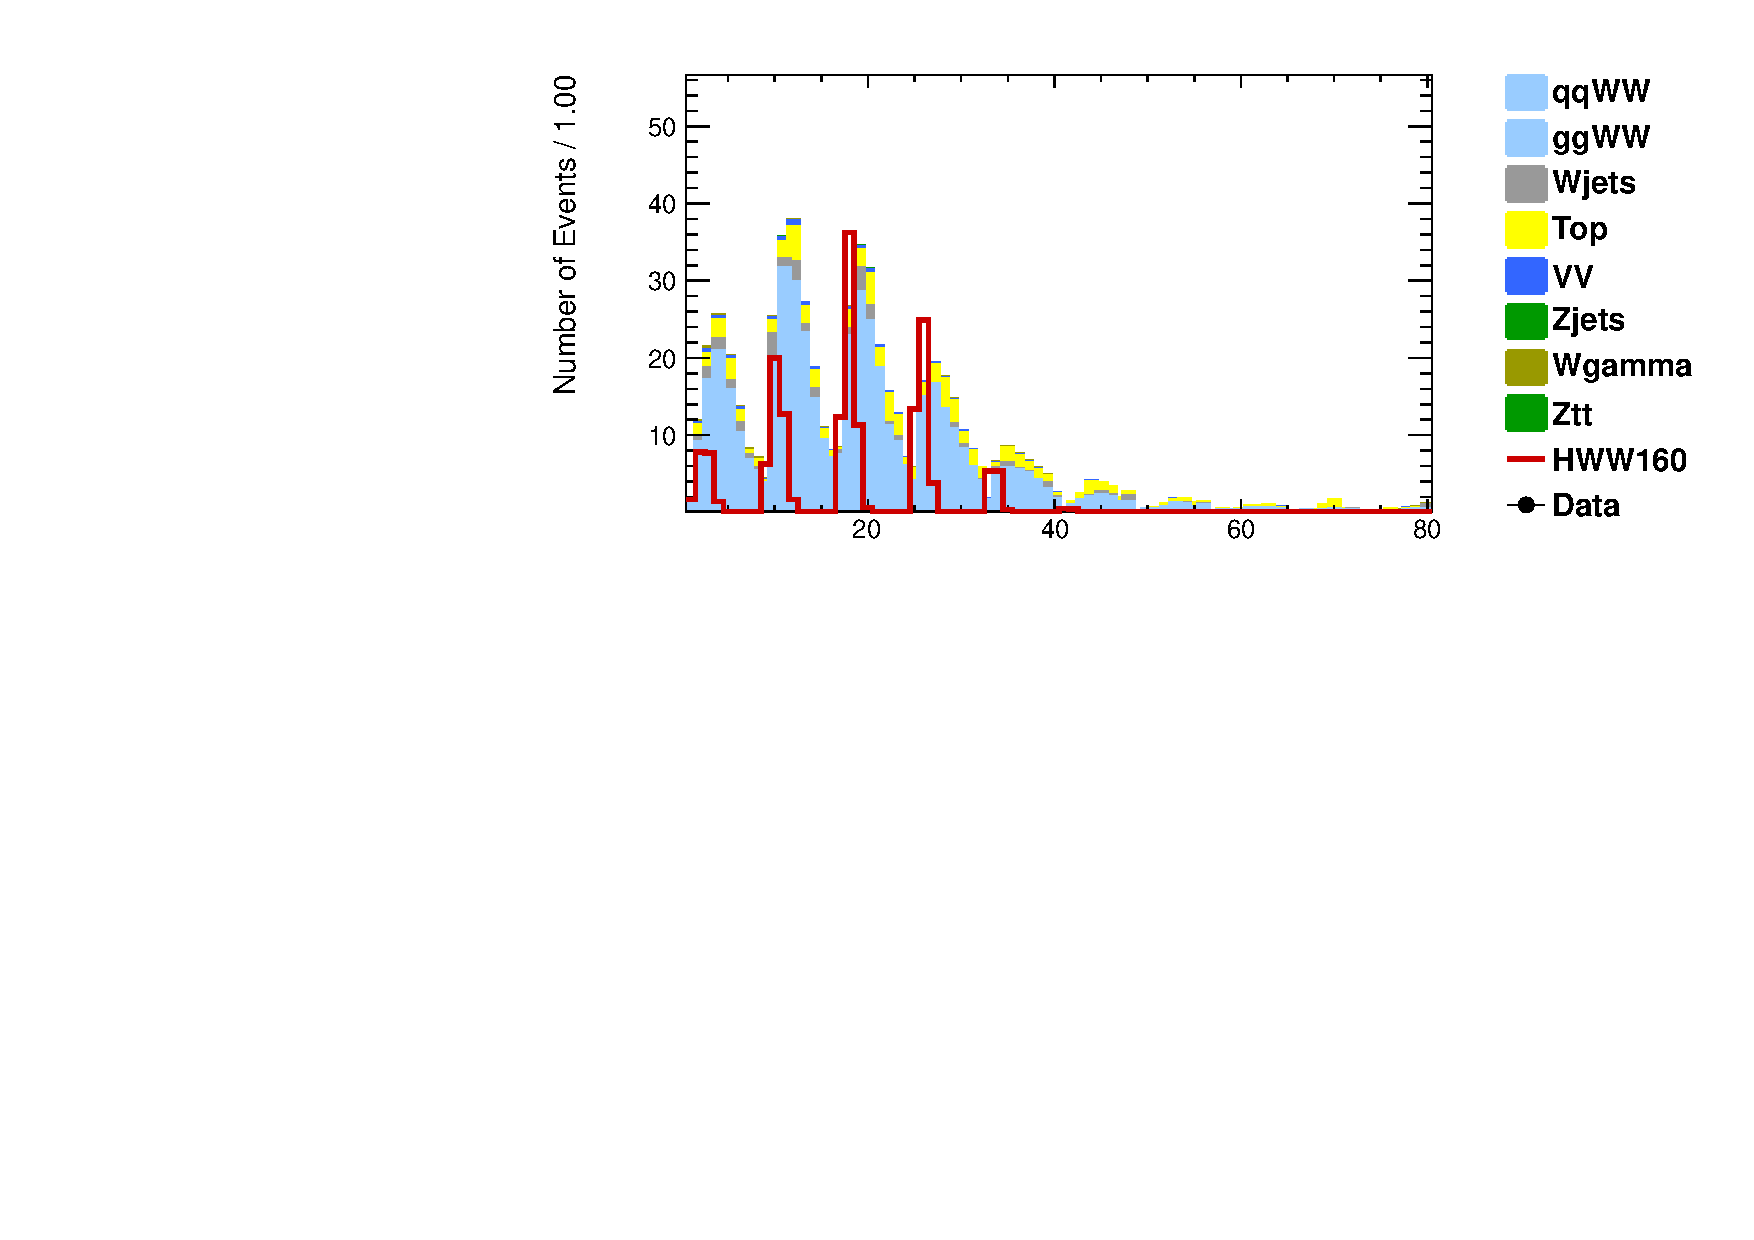
\includegraphics[width=.45\textwidth]{figures/templates/2D_mH160_0j_of_stack_lin.pdf}
	}
	\subfigure[Overlaid unrolled template linear]{
	\centering
	\label{subfig:template_unroll_overlay_lin}
		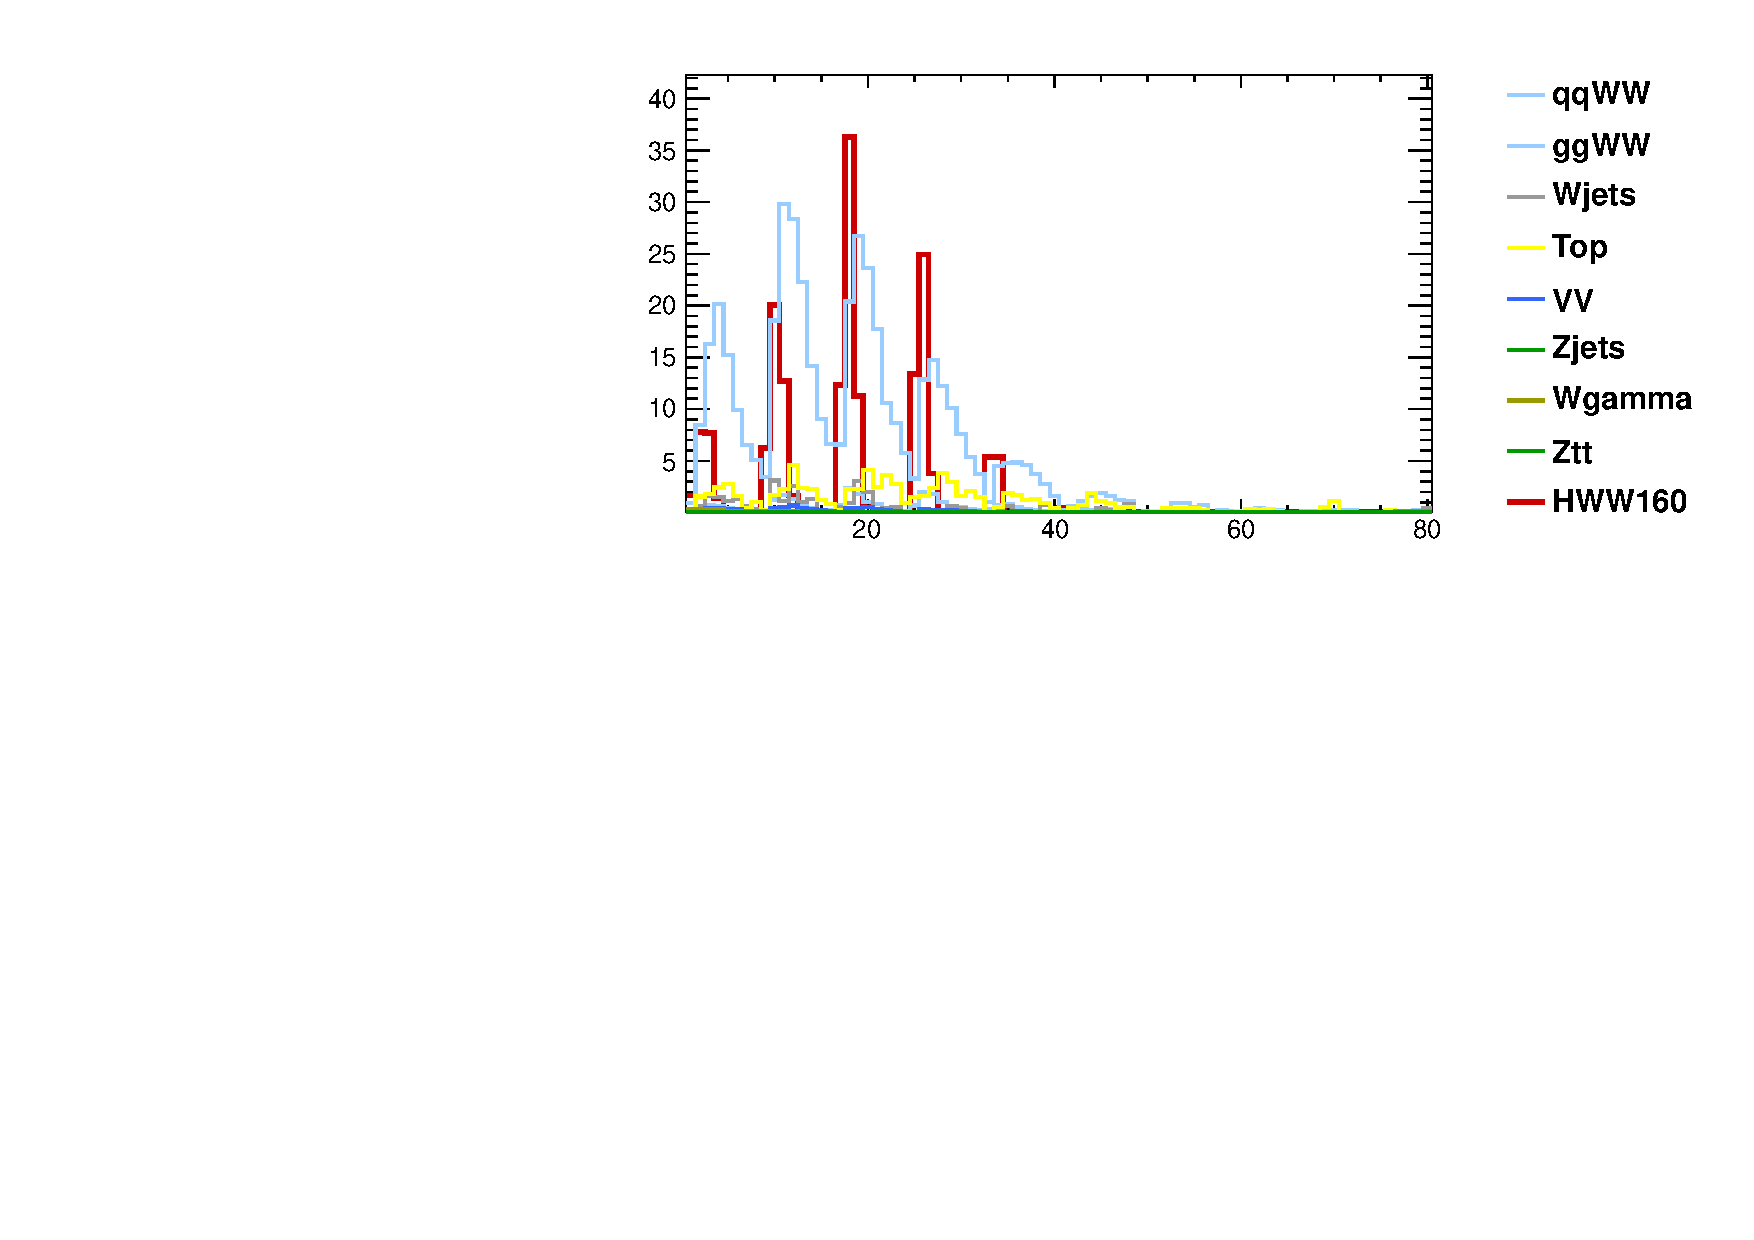
\includegraphics[width=.45\textwidth]{figures/templates/2D_mH160_0j_of_overlay_lin.pdf}
	}

	%
	\centering
	\subfigure[Stacked unrolled template in log scale]{
	\centering
	\label{subfig:template_unroll_stack_log}
		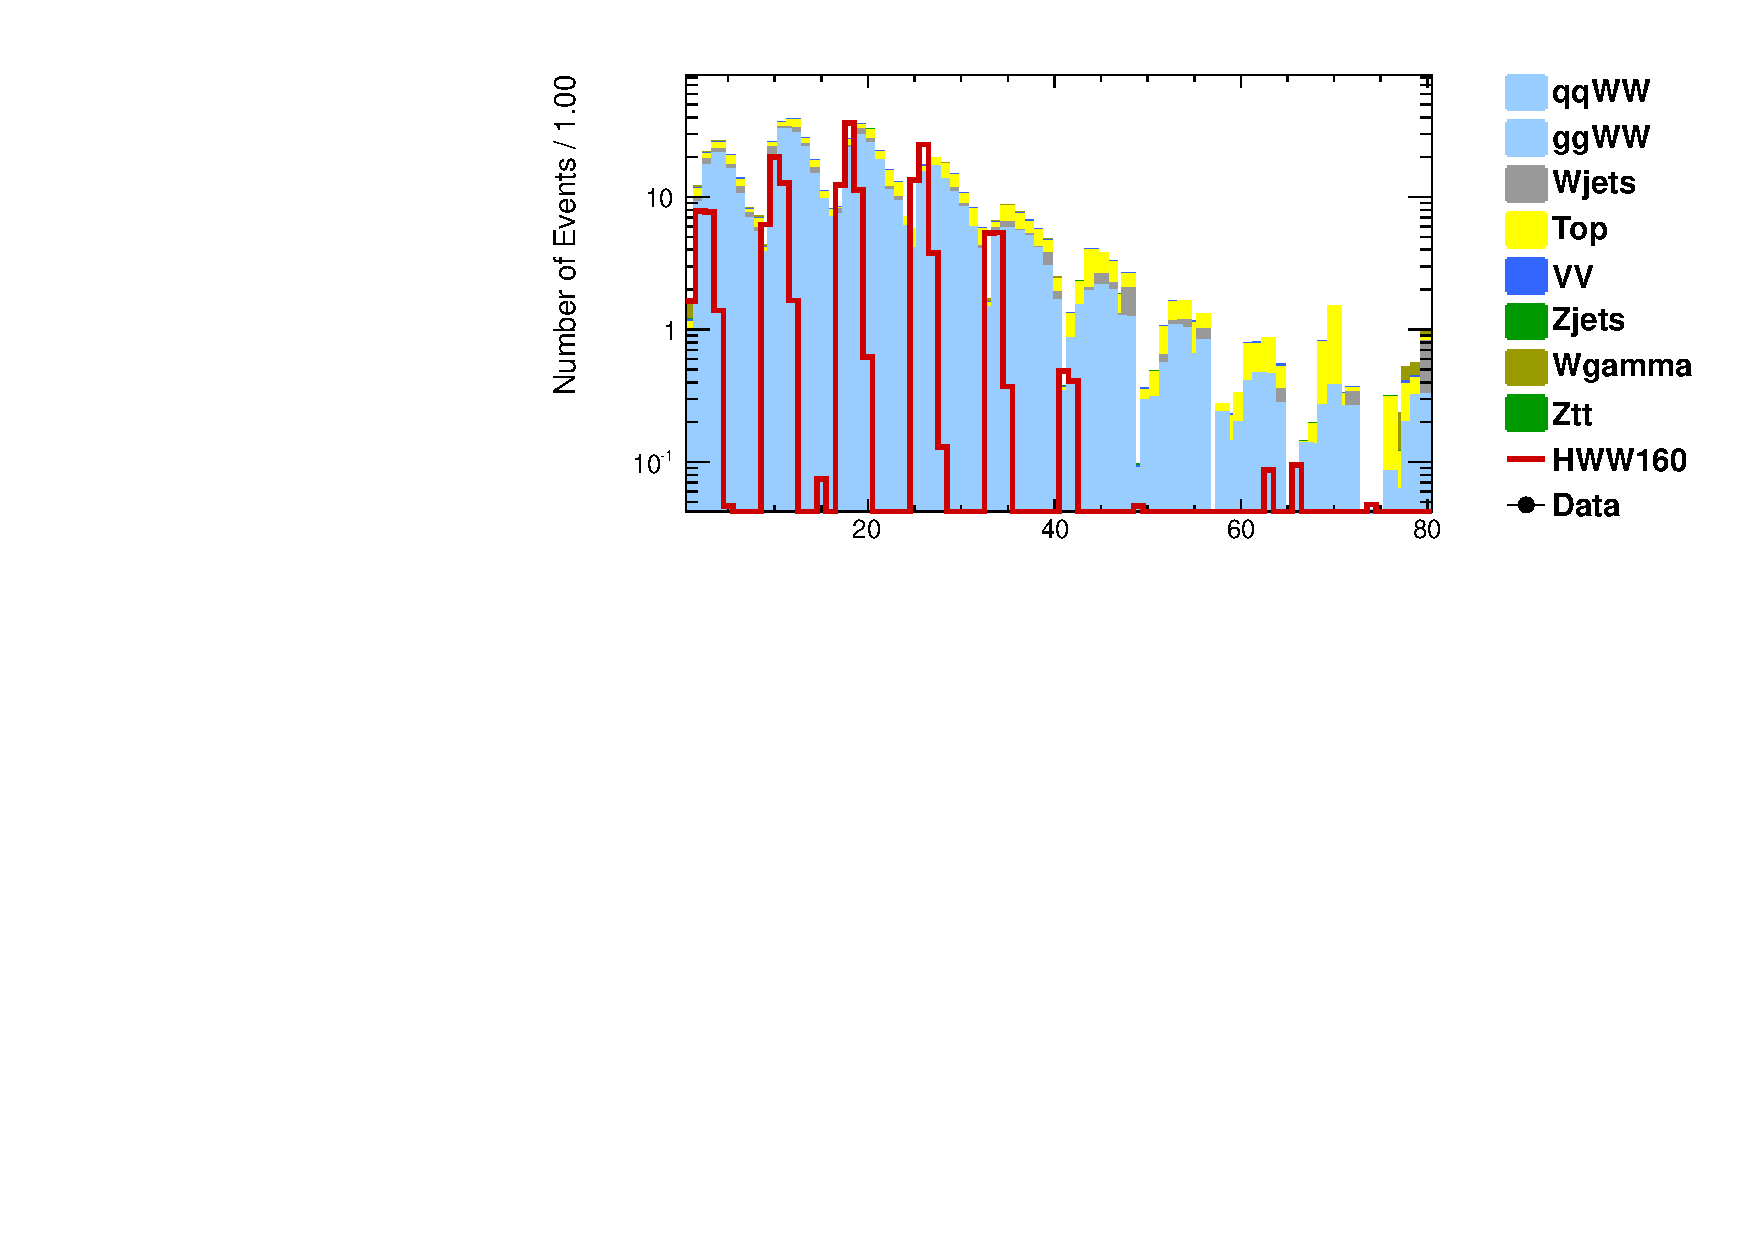
\includegraphics[width=.45\textwidth]{figures/templates/2D_mH160_0j_of_stack_log.pdf}
	}
	\subfigure[Overlaid unrolled template in log scale]{
	\centering
	\label{subfig:template_unroll_overlay_log}
		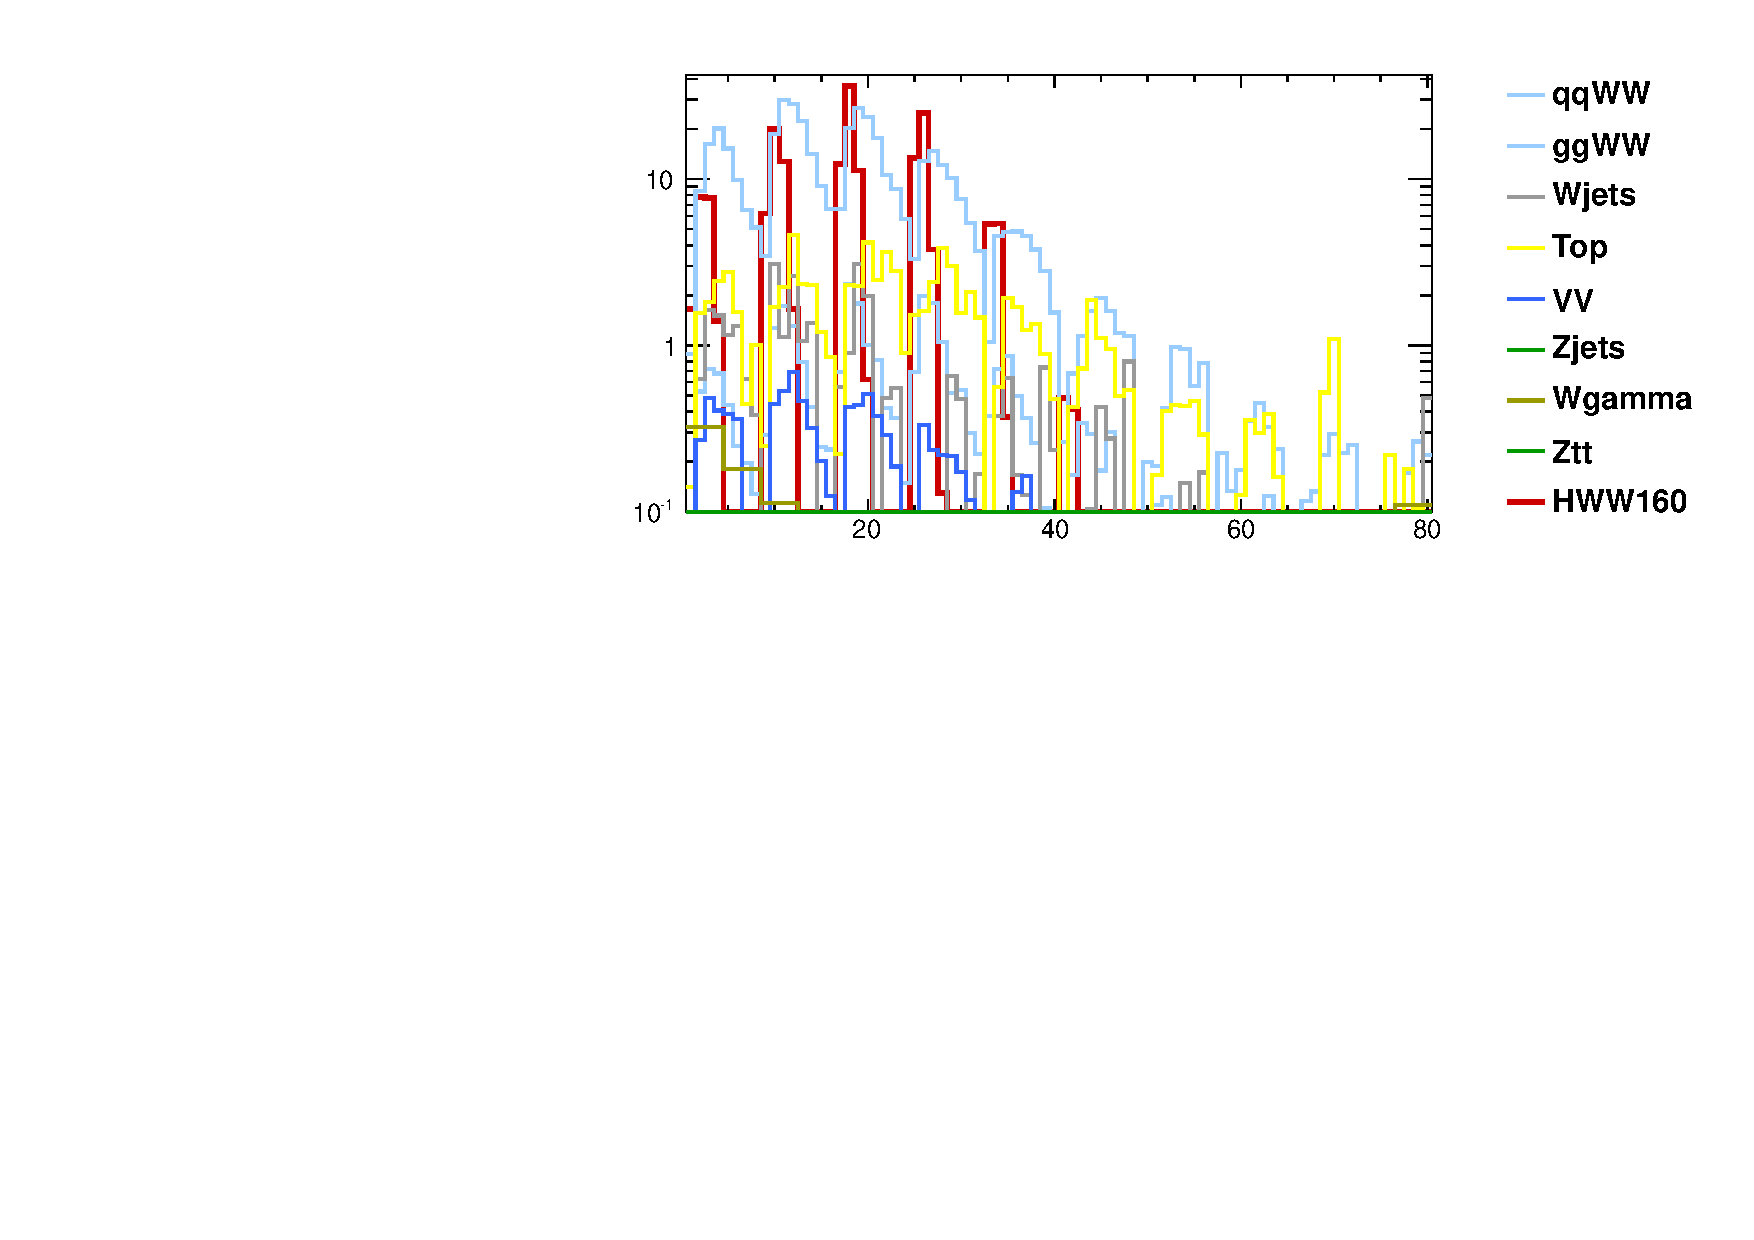
\includegraphics[width=.45\textwidth]{figures/templates/2D_mH160_0j_of_overlay_log.pdf}
	}

	\caption{Unrolled templates at \mHi = 160 \GeV} 
	\label{fig:templates_160_unroll}

\end{figure} 

%%%%%% mH=200 GeV
\begin{figure}[!hbtp]
	
	%
	\centering
	\subfigure[Signal]{
	\centering
	\label{subfig:template_signal_200}
		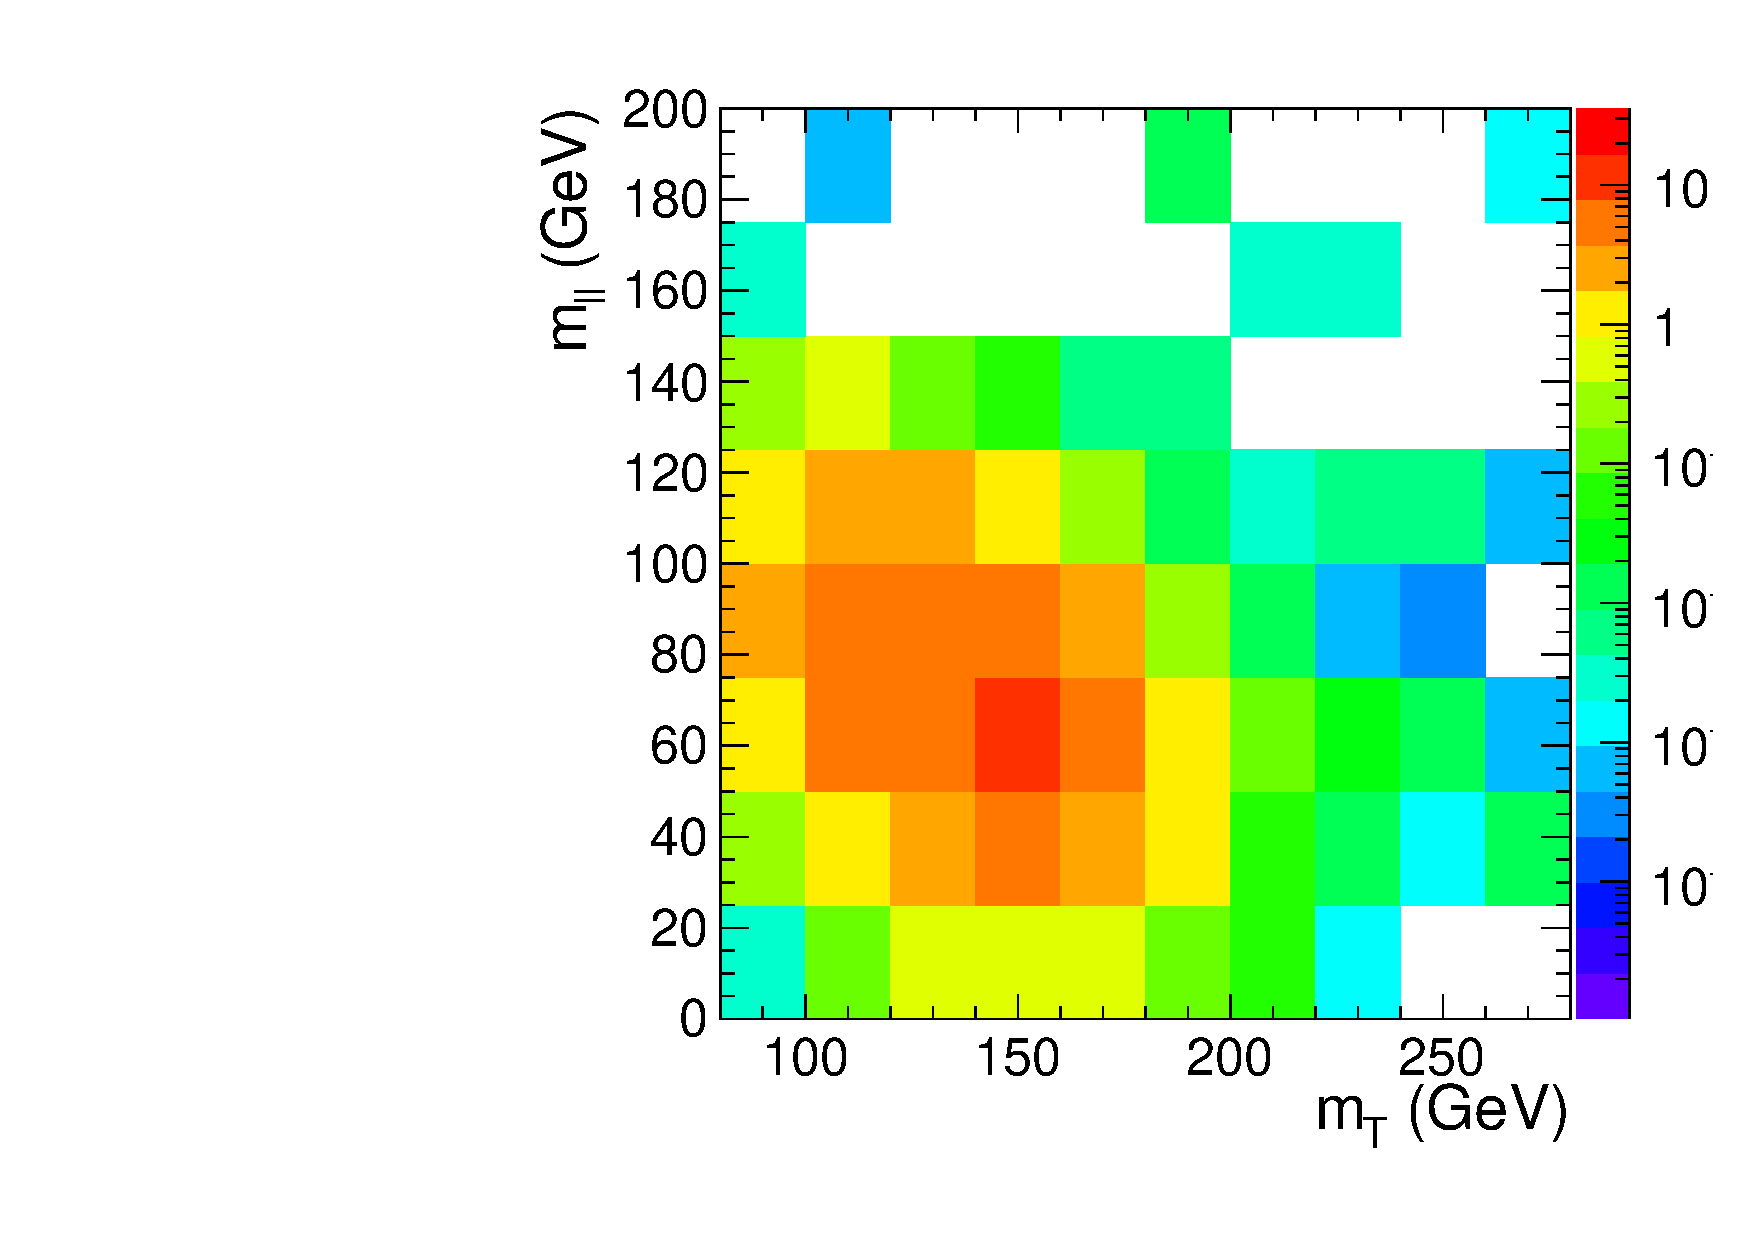
\includegraphics[width=.35\textwidth]{figures/templates/sig_2D_mH200_0j_of.pdf}
	}
	\subfigure[Signal statistical uncertainty]{
	\centering
	\label{subfig:template_signalerr_200}
		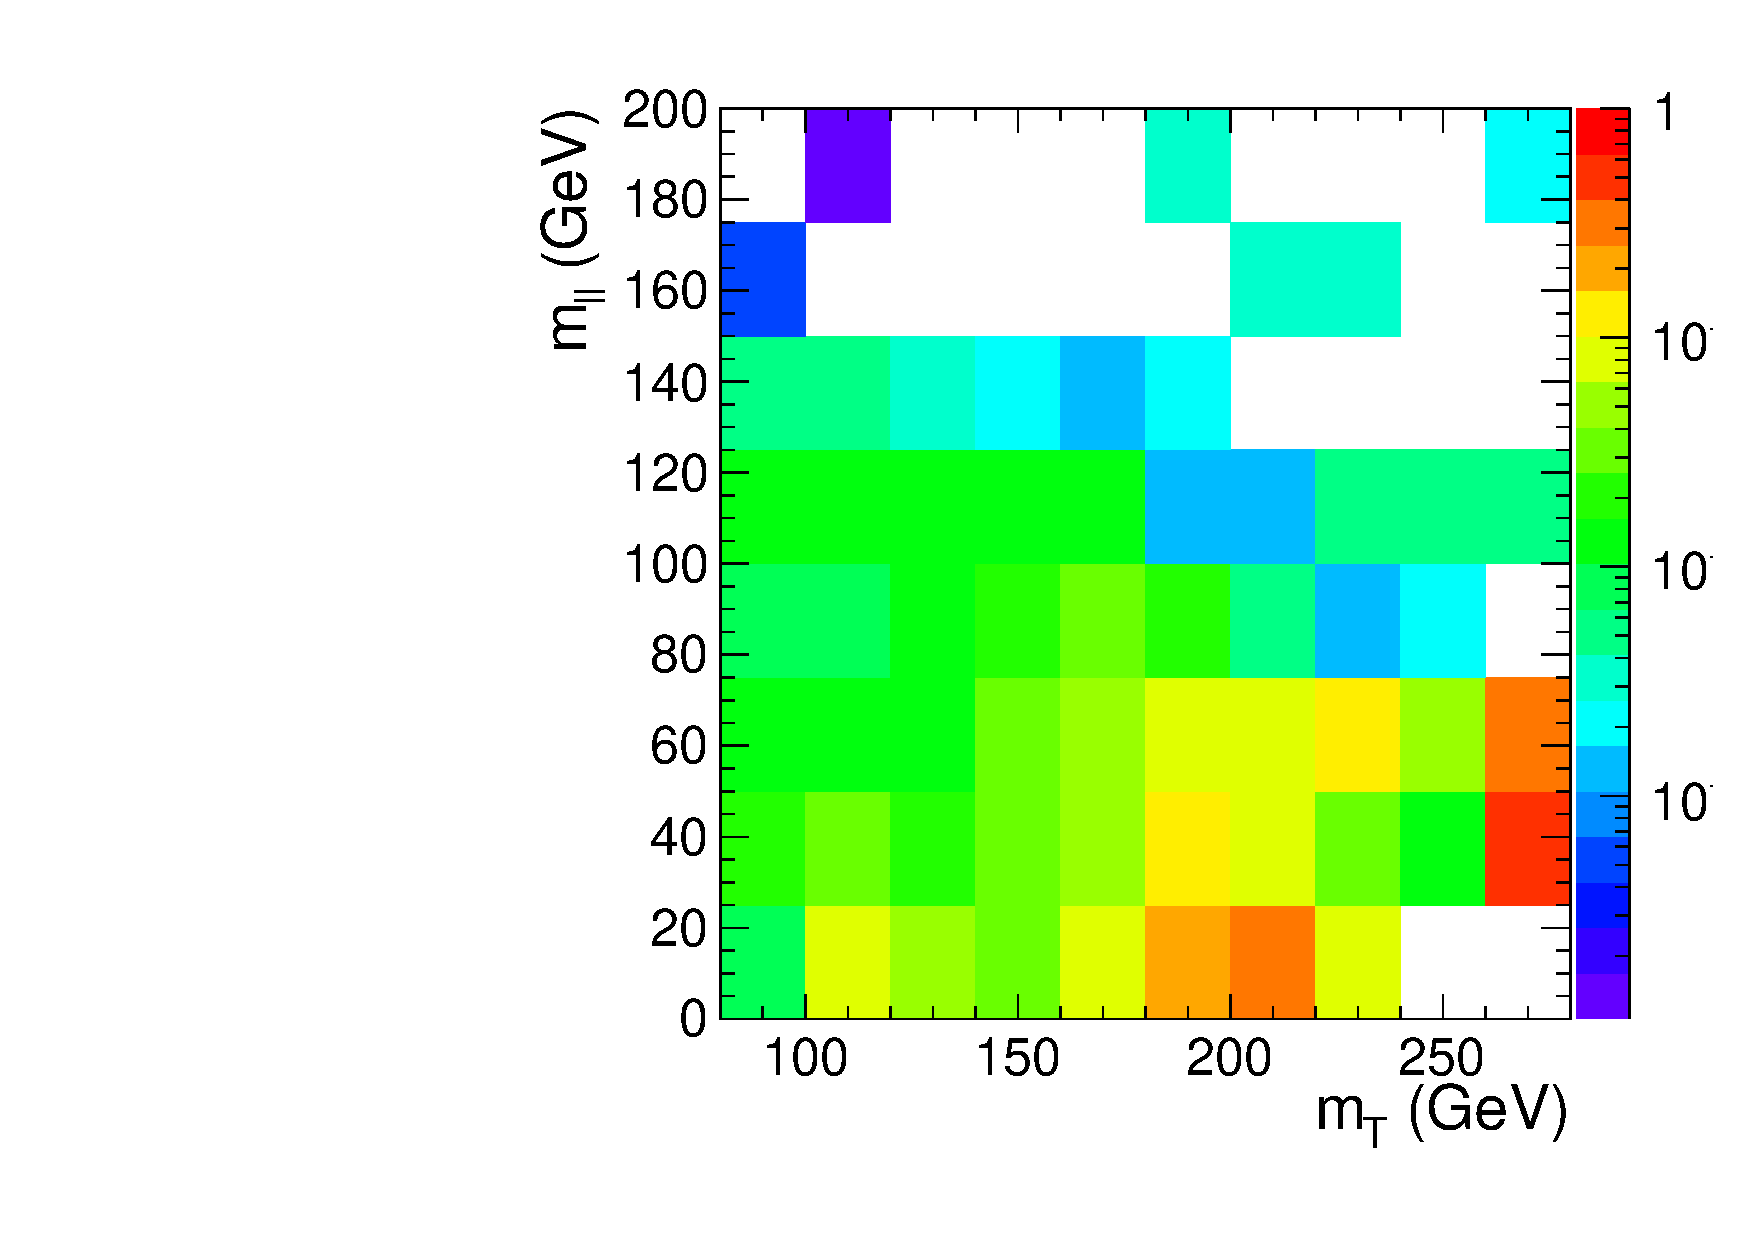
\includegraphics[width=.35\textwidth]{figures/templates/sigerr_2D_mH200_0j_of.pdf}
	}
	
	%
	\centering
	\subfigure[qqWW]{
	\centering
	\label{subfig:template_qqWW_200}
		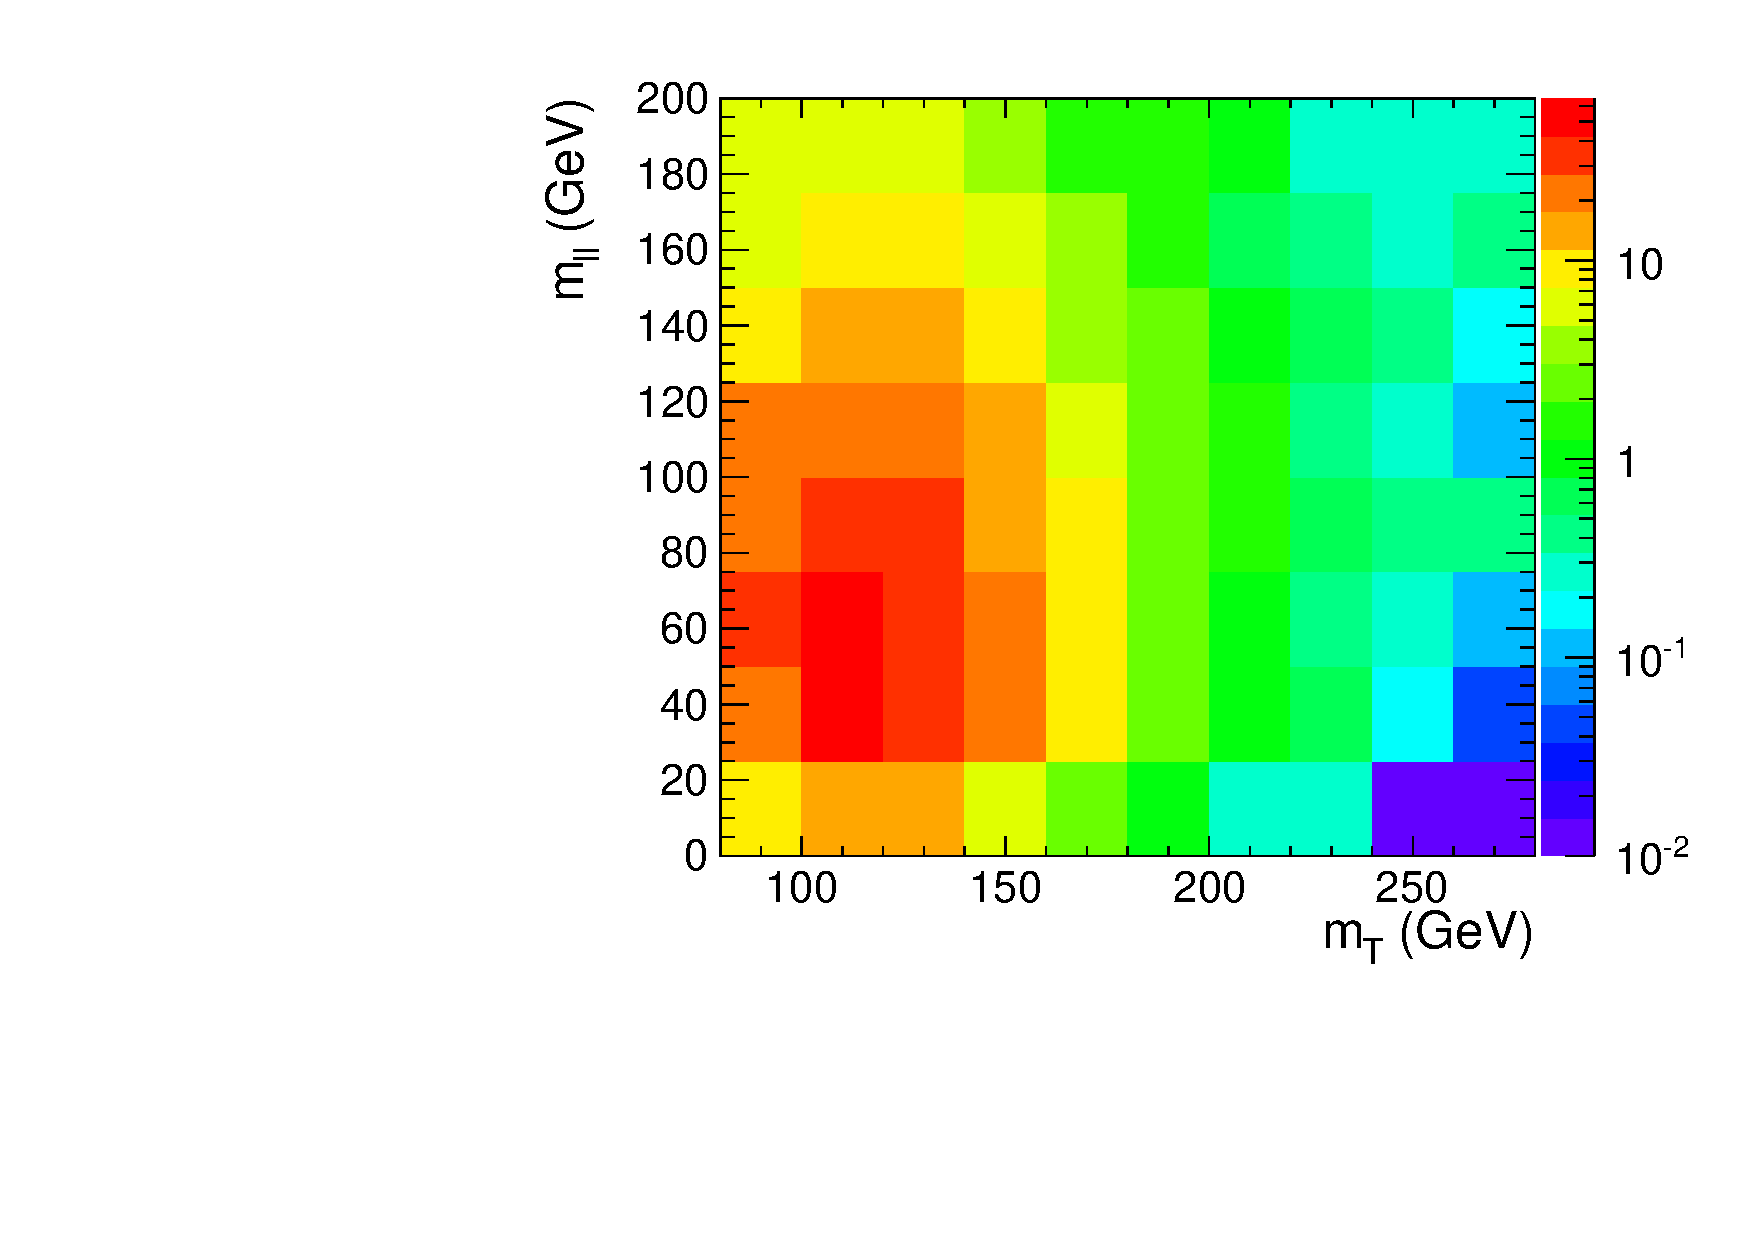
\includegraphics[width=.35\textwidth]{figures/templates/qqWW_2D_mH200_0j_of.pdf}
	}
	\subfigure[qqWW statistical uncertainty]{
	\centering
	\label{subfig:template_qqWWerr_200}
		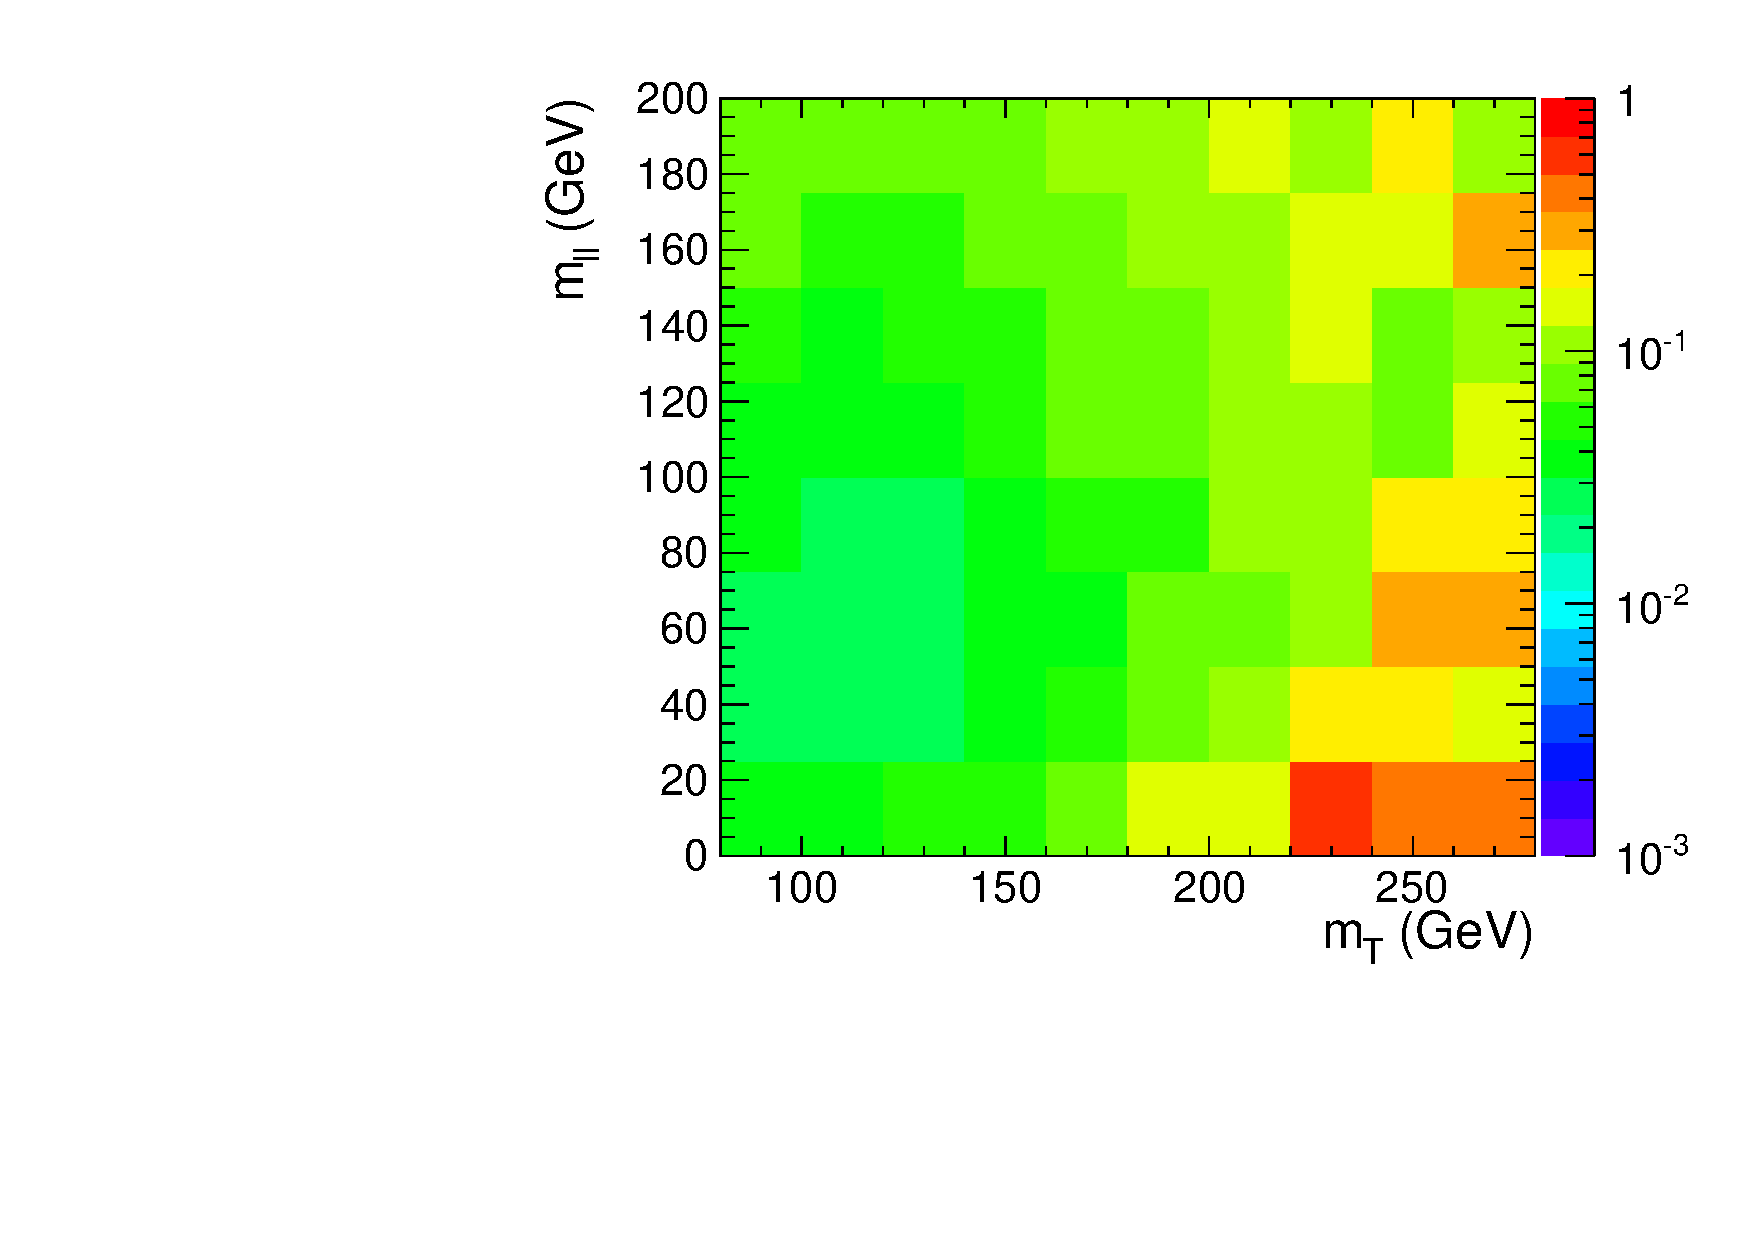
\includegraphics[width=.35\textwidth]{figures/templates/qqWWerr_2D_mH200_0j_of.pdf}
	}

	%
	\centering
	\subfigure[ggWW]{
	\centering
	\label{subfig:template_ggWW_200}
		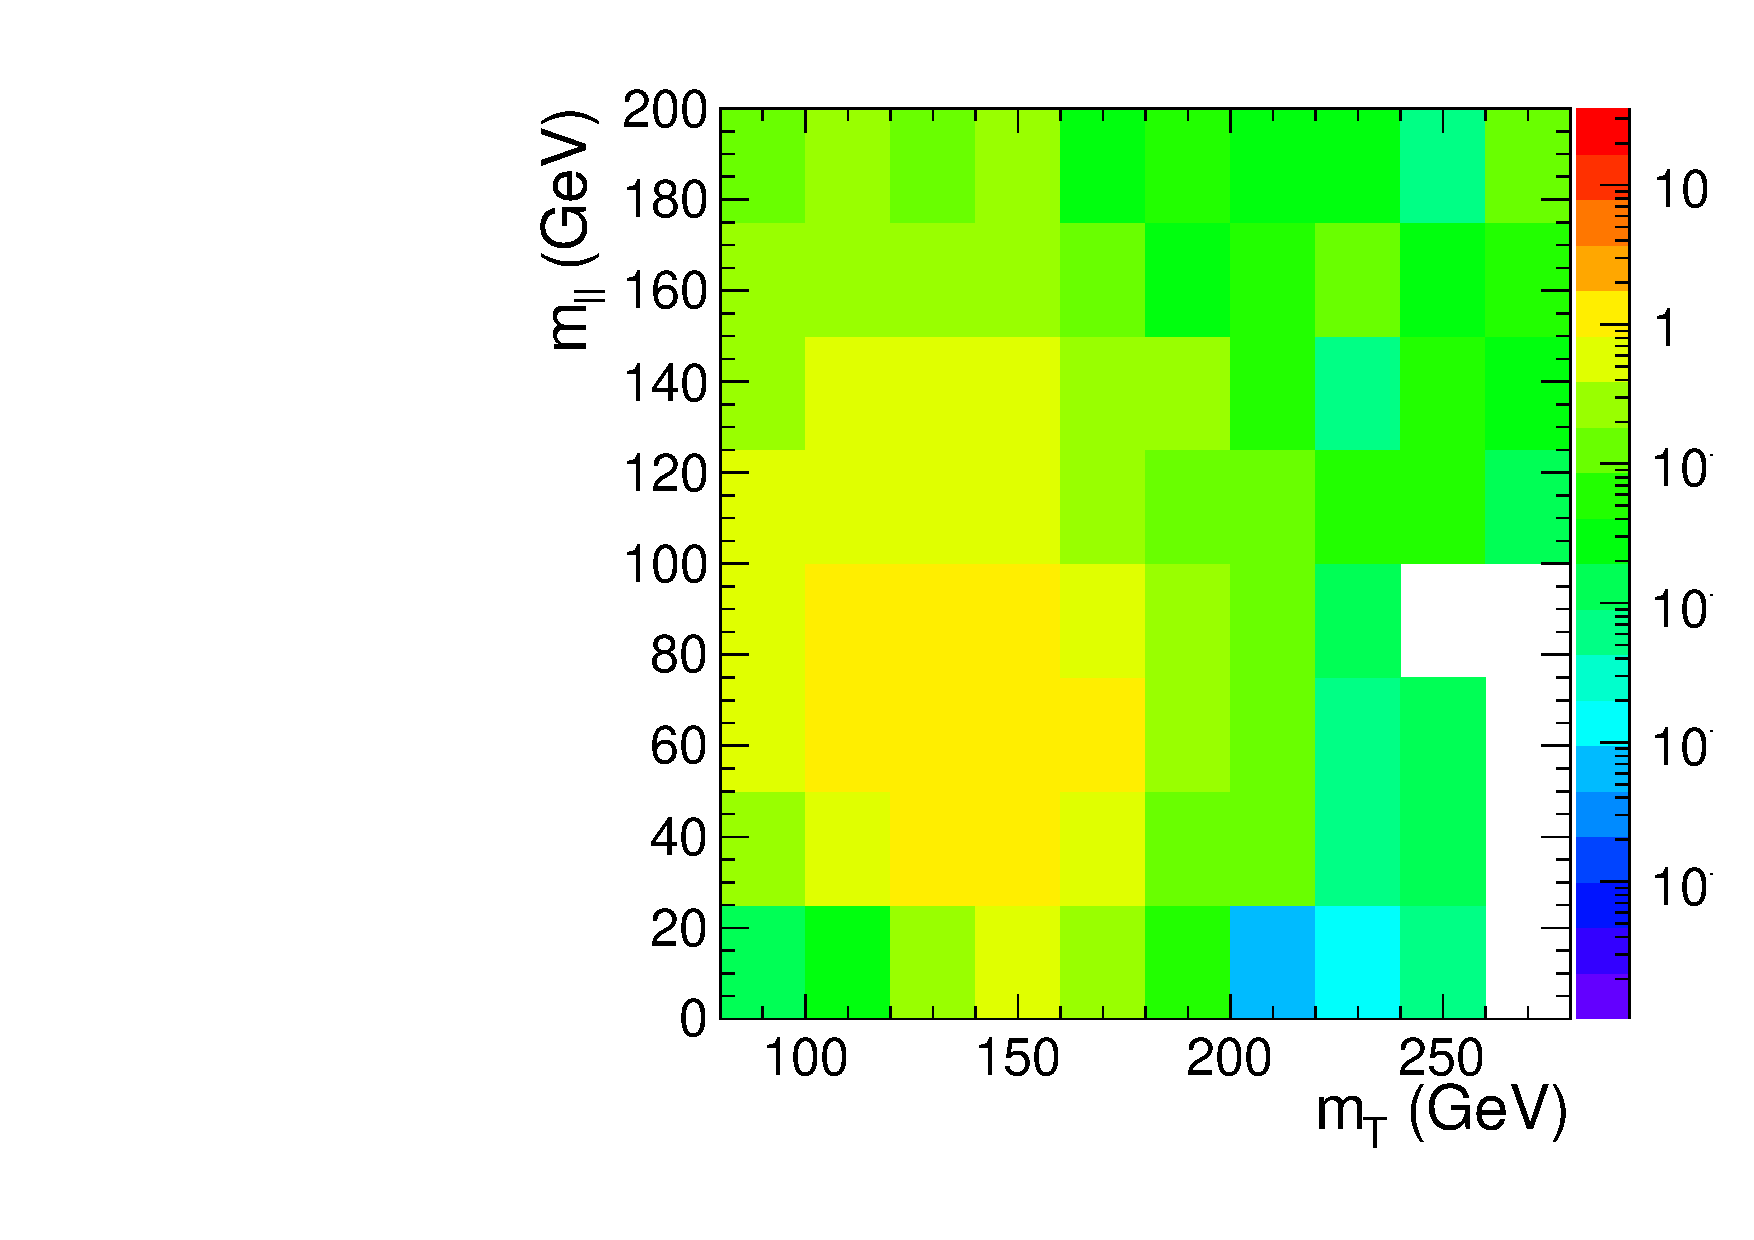
\includegraphics[width=.35\textwidth]{figures/templates/ggWW_2D_mH200_0j_of.pdf}
	}
	\subfigure[ggWW statistical uncertainty]{
	\centering
	\label{subfig:template_ggWWerr_200}
		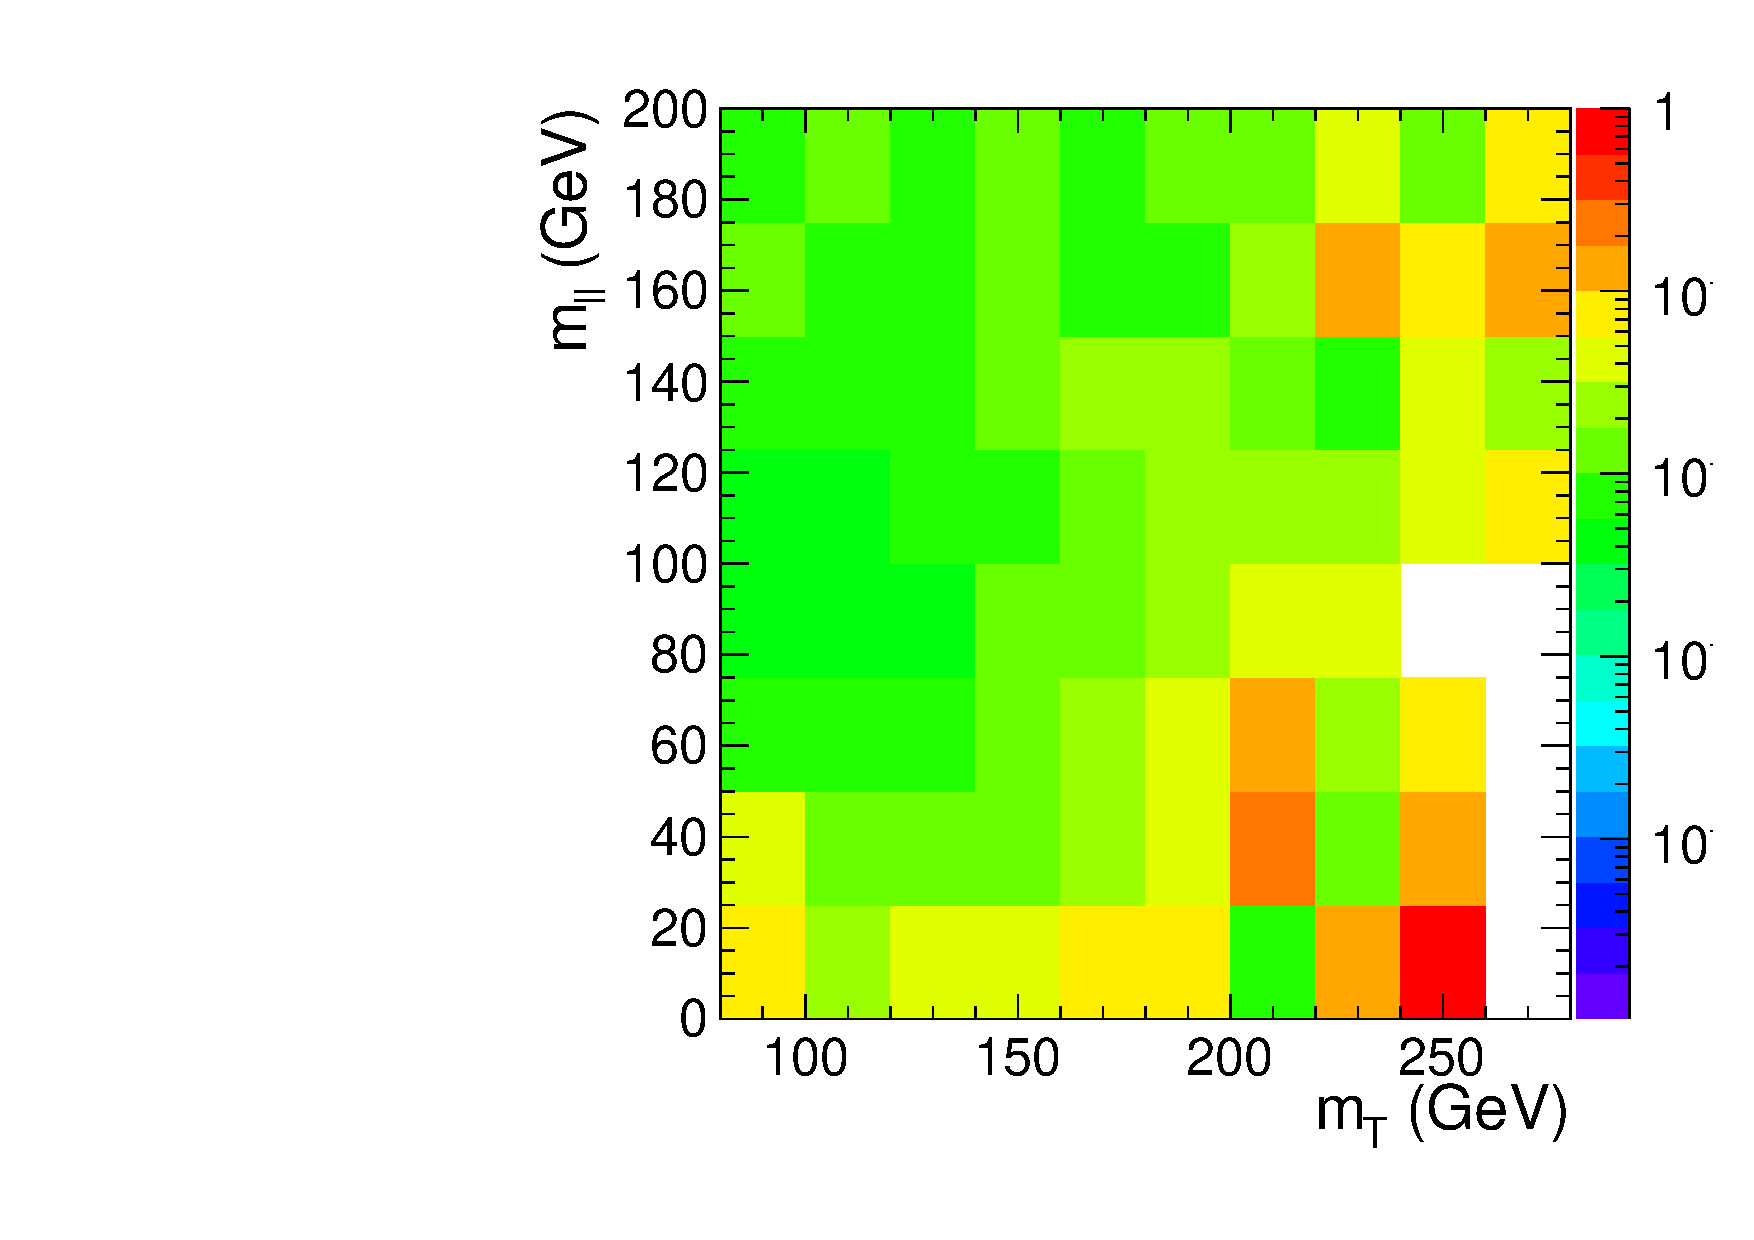
\includegraphics[width=.35\textwidth]{figures/templates/ggWWerr_2D_mH200_0j_of.pdf}
	}

	\caption{2D templates at \mHi = 200 \GeV} 
	\label{fig:templates_200_1}

\end{figure}

\begin{figure}[!hbtp]
	
	%
	\centering
	\subfigure[Wjets]{
	\centering
	\label{subfig:template_Wjets_200}
		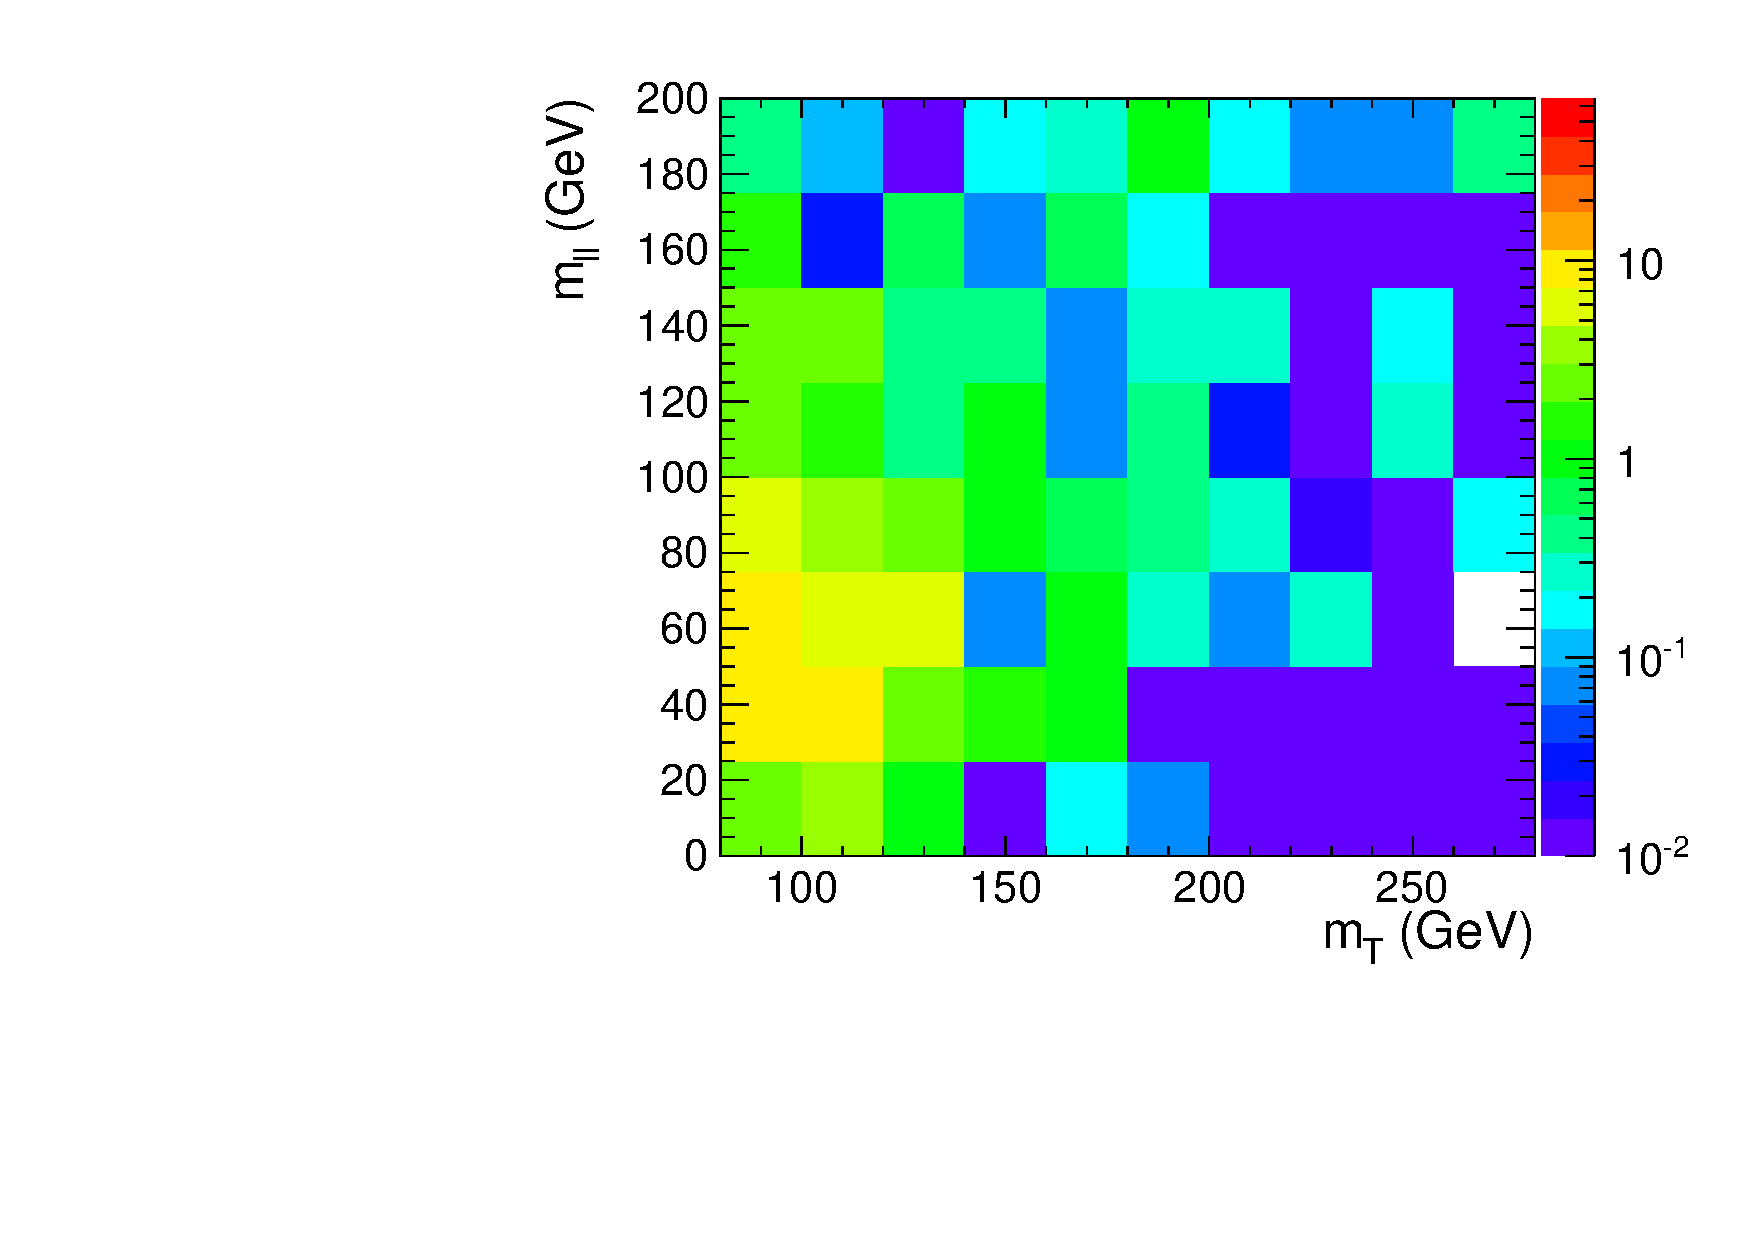
\includegraphics[width=.35\textwidth]{figures/templates/Wjets_2D_mH200_0j_of.pdf}
	}
	\subfigure[Wjets statistical uncertainty]{
	\centering
	\label{subfig:template_Wjetserr_200}
		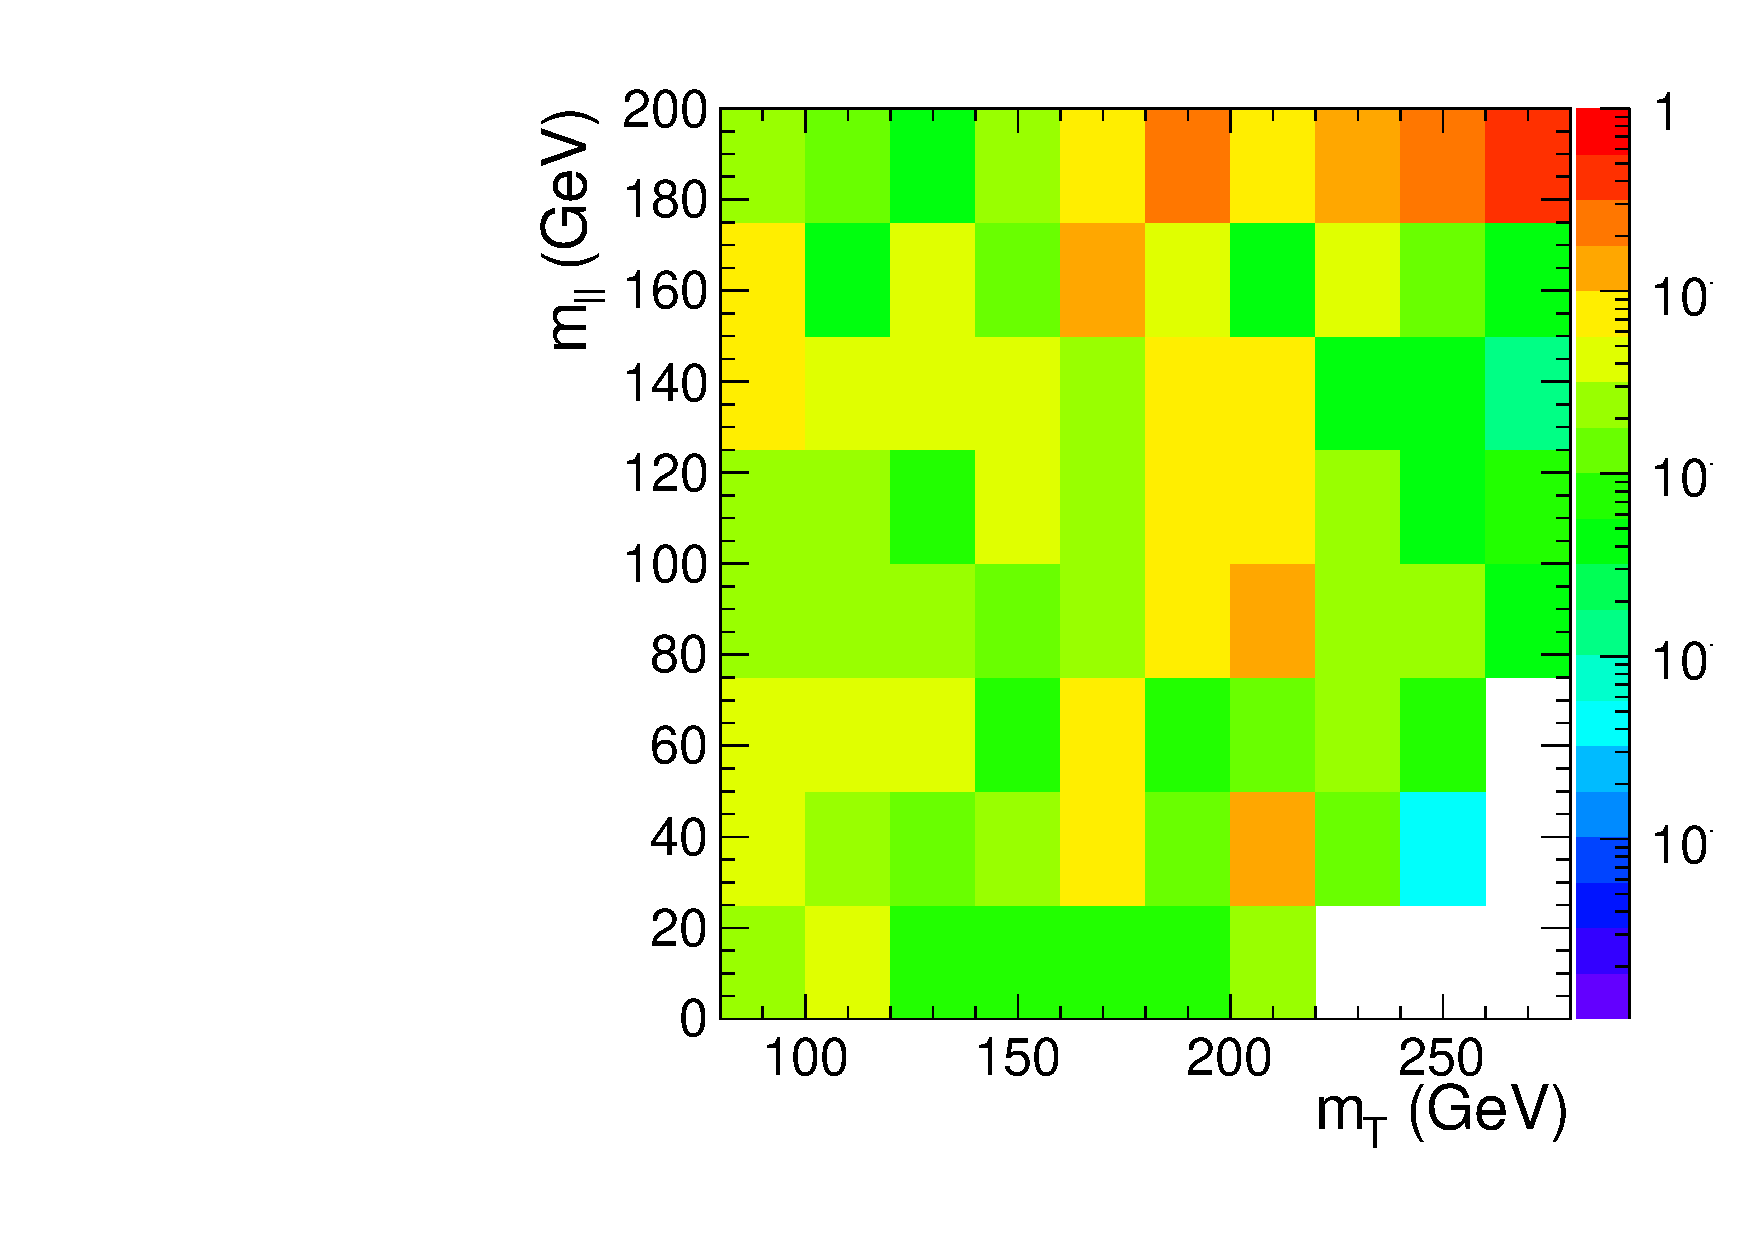
\includegraphics[width=.35\textwidth]{figures/templates/Wjetserr_2D_mH200_0j_of.pdf}
	}
	
	%
	\centering
	\subfigure[Top]{
	\centering
	\label{subfig:template_Top_200}
		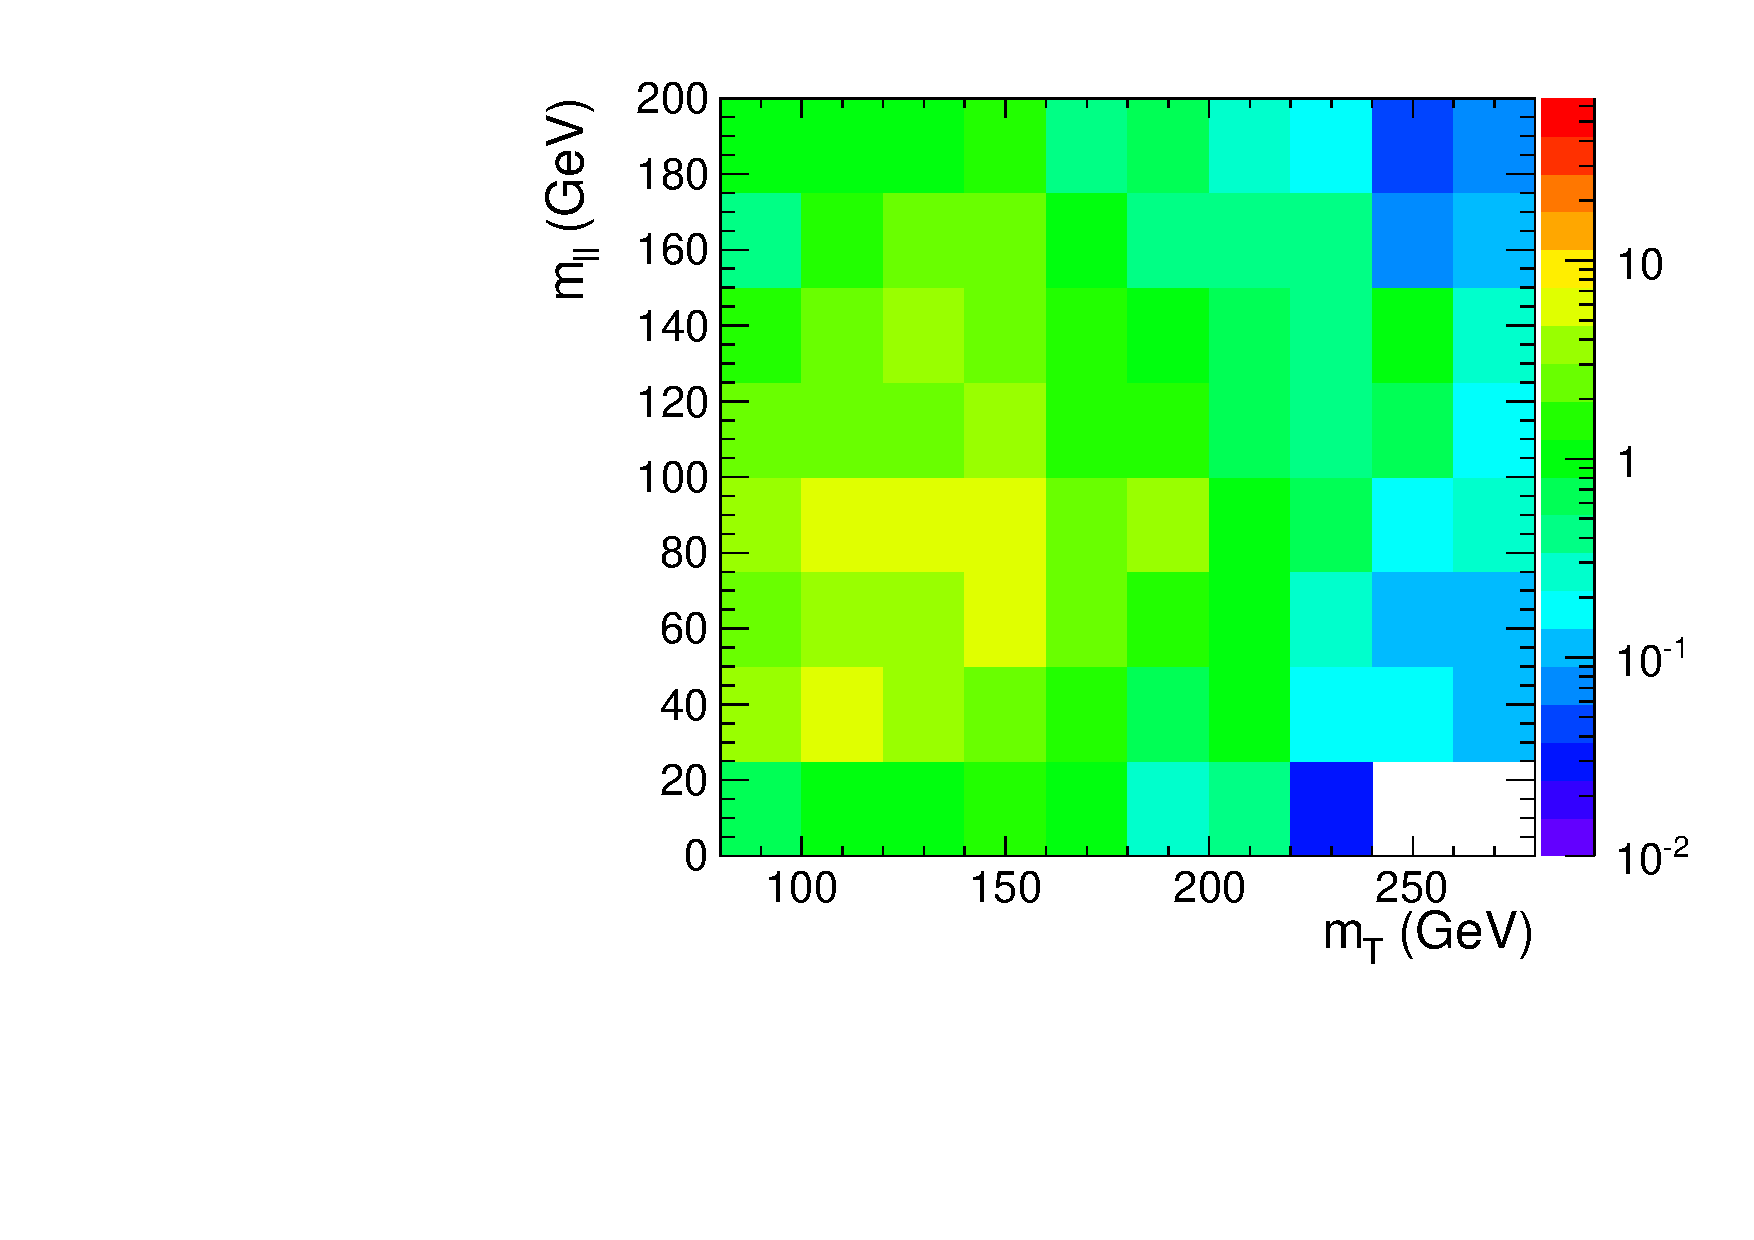
\includegraphics[width=.35\textwidth]{figures/templates/Top_2D_mH200_0j_of.pdf}
	}
	\subfigure[Top statistical uncertainty]{
	\centering
	\label{subfig:template_Toperr_200}
		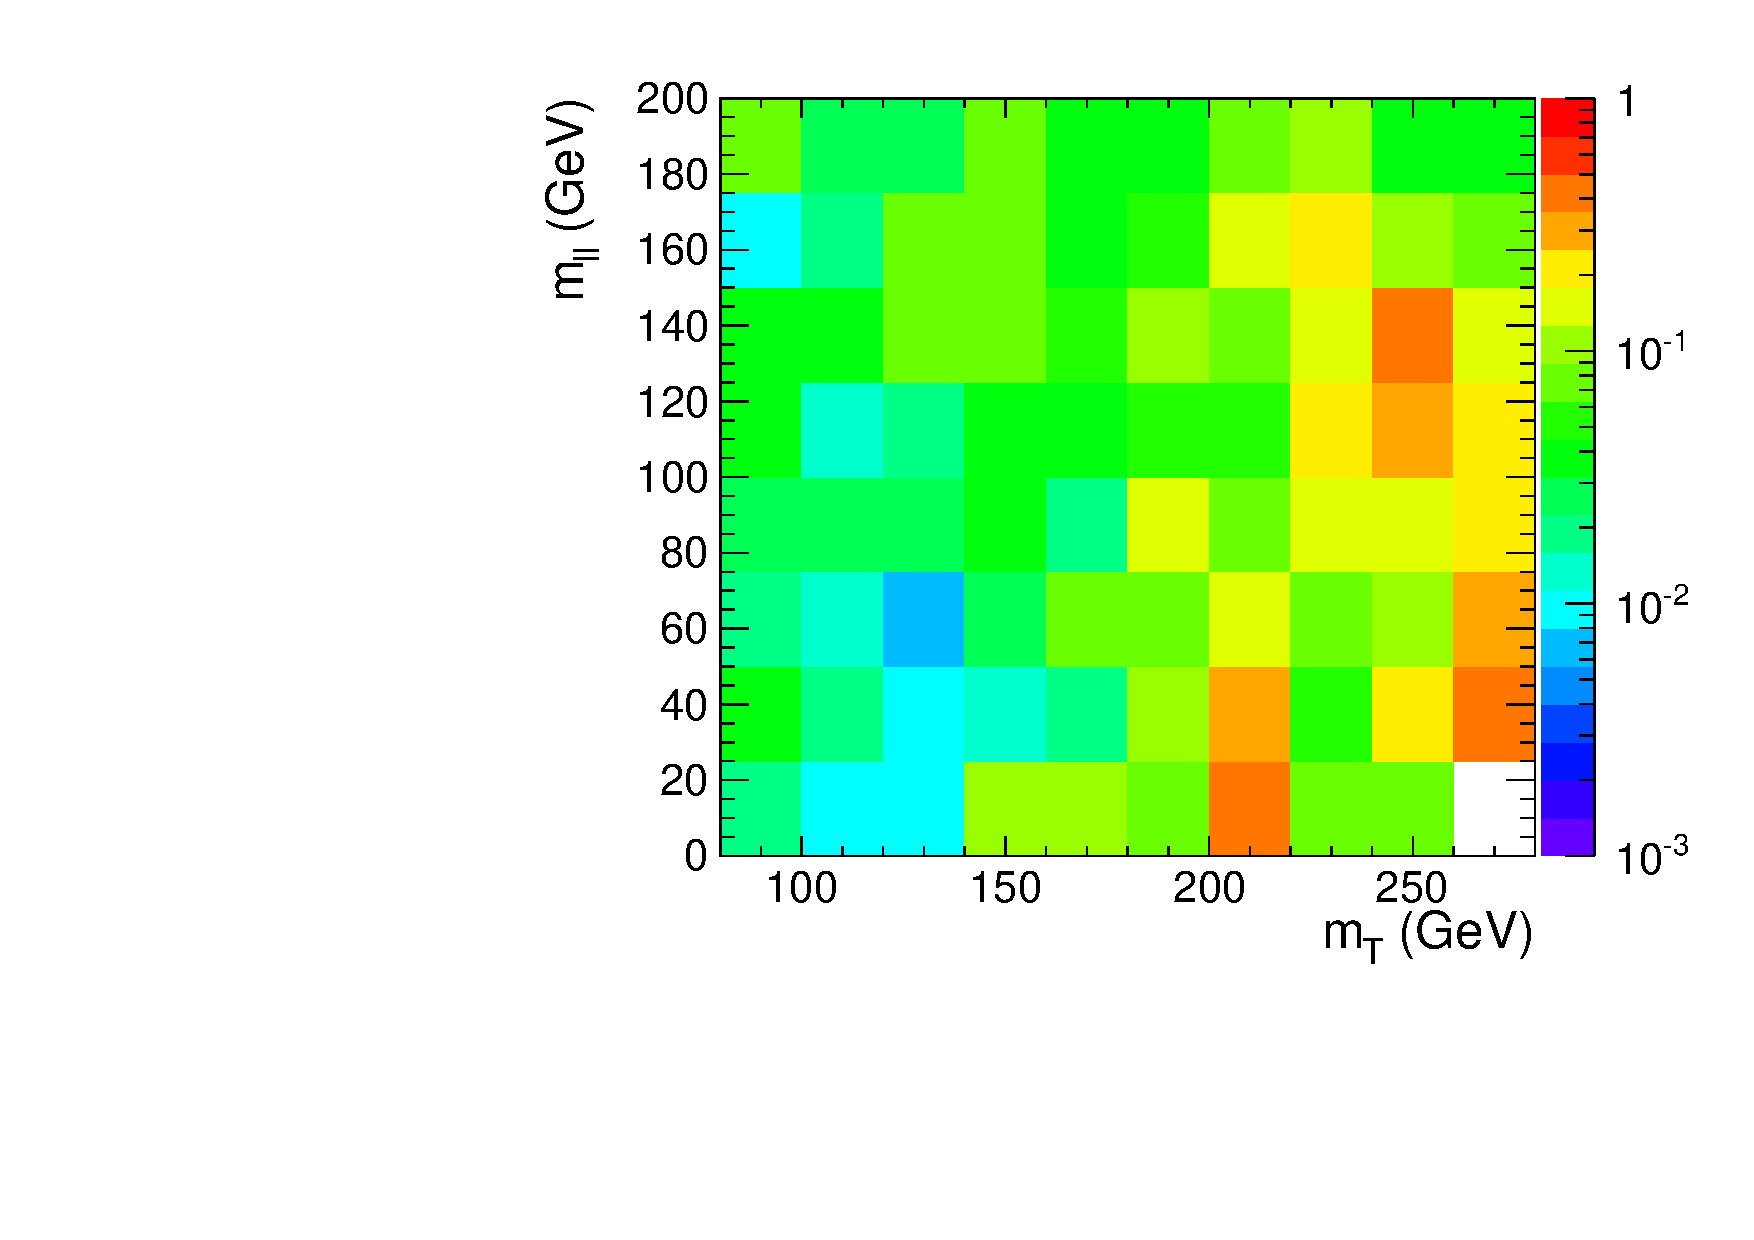
\includegraphics[width=.35\textwidth]{figures/templates/Toperr_2D_mH200_0j_of.pdf}
	}

	%
	\centering
	\subfigure[VV]{
	\centering
	\label{subfig:template_VV_200}
		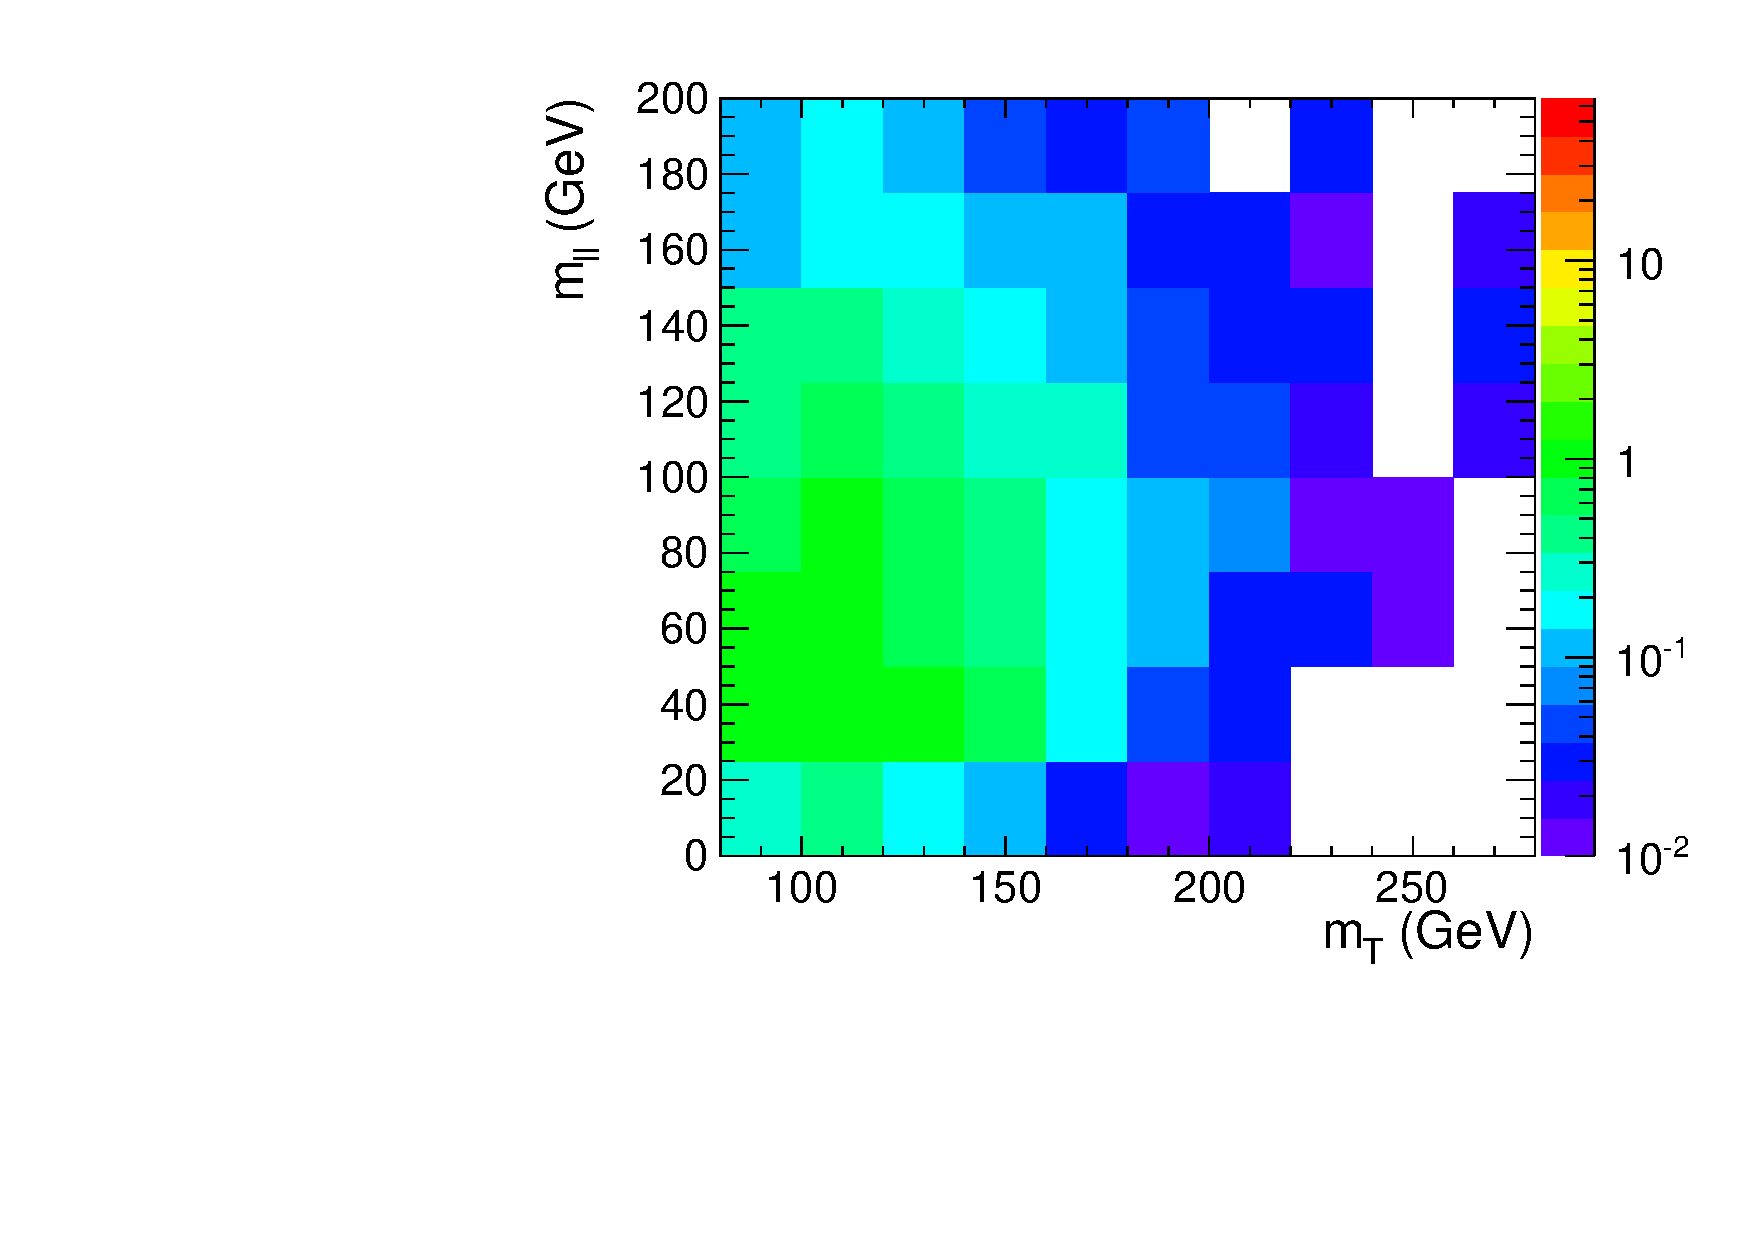
\includegraphics[width=.35\textwidth]{figures/templates/VV_2D_mH200_0j_of.pdf}
	}
	\subfigure[VV statistical uncertainty]{
	\centering
	\label{subfig:template_VVerr_200}
		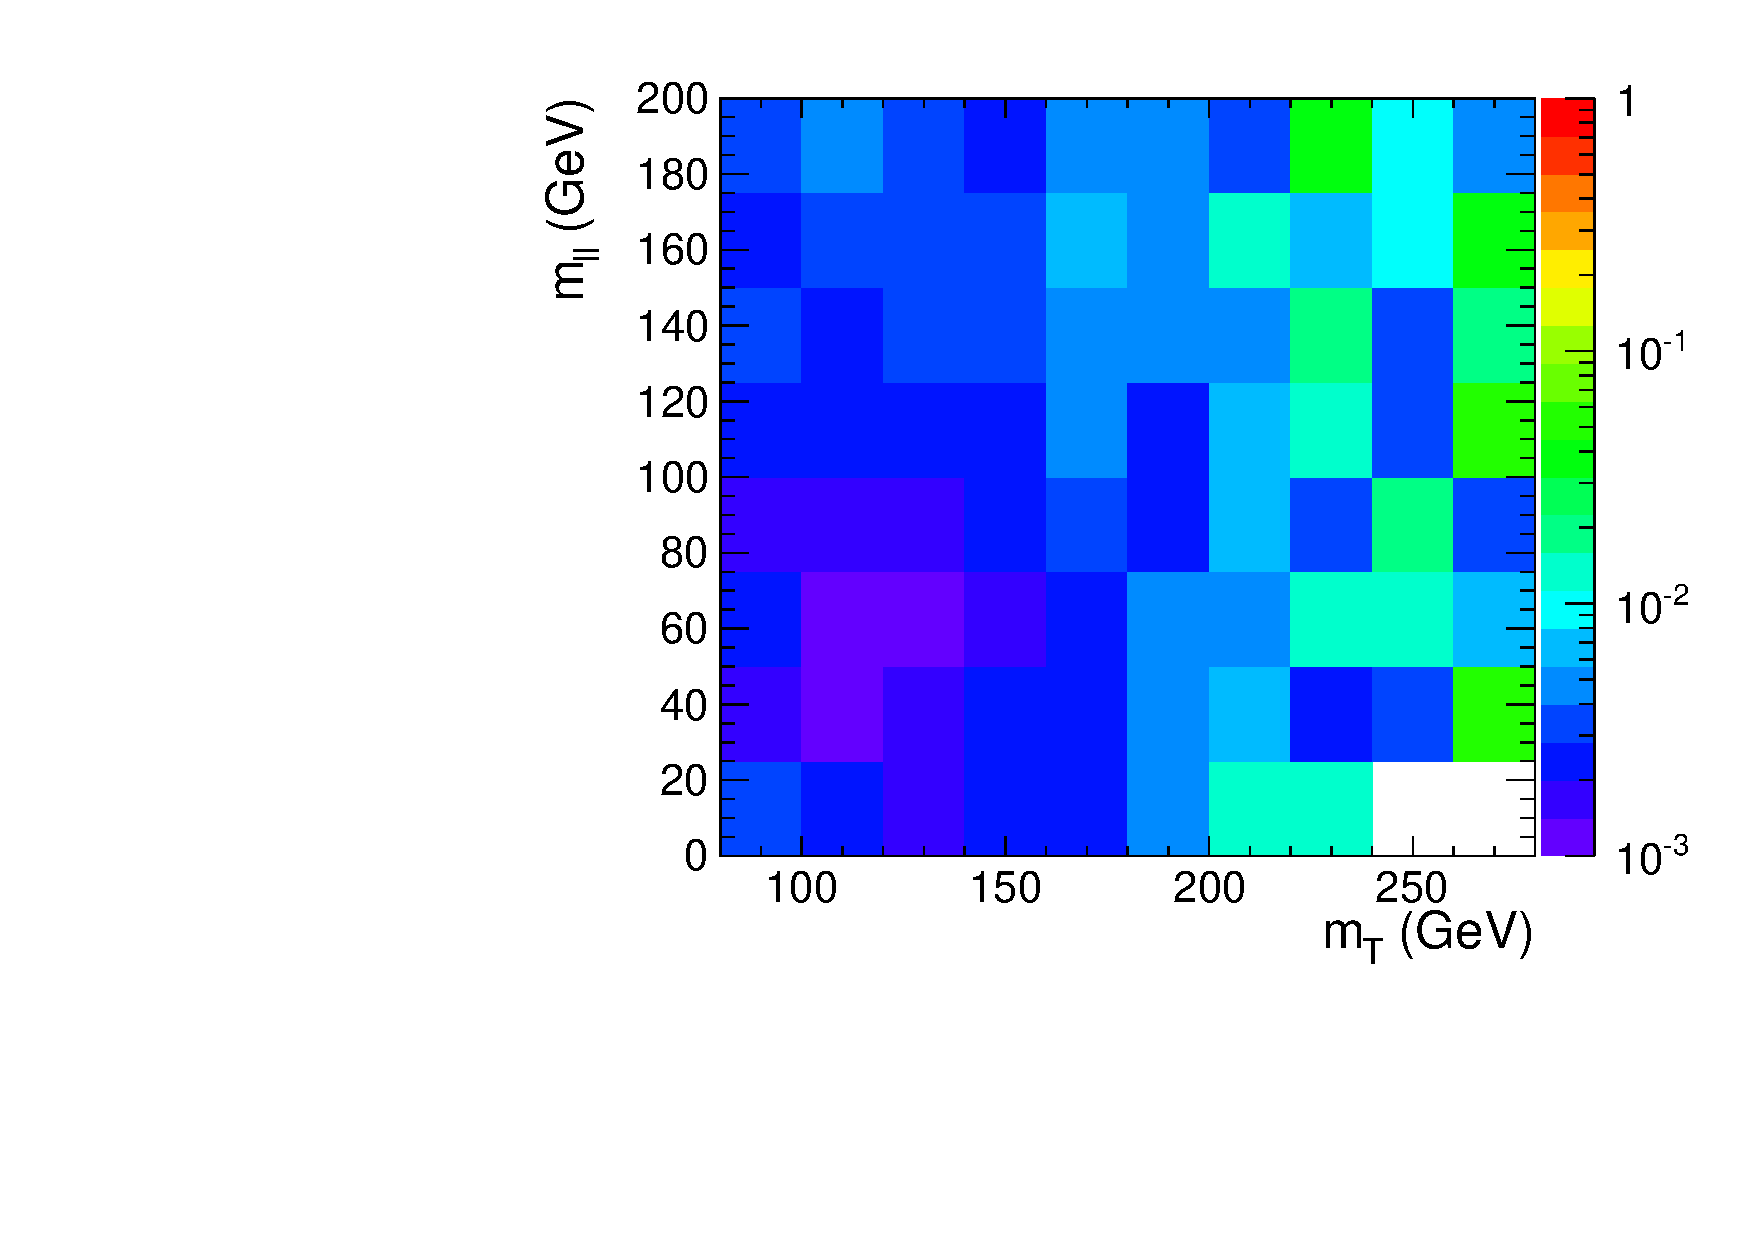
\includegraphics[width=.35\textwidth]{figures/templates/VVerr_2D_mH200_0j_of.pdf}
	}

	\caption{2D templates at \mHi = 200 \GeV} 
	\label{fig:templates_200_2}

\end{figure}

\begin{figure}[!hbtp]
	
	%
	\centering
	\subfigure[Zjets]{
	\centering
	\label{subfig:template_Zjets_200}
		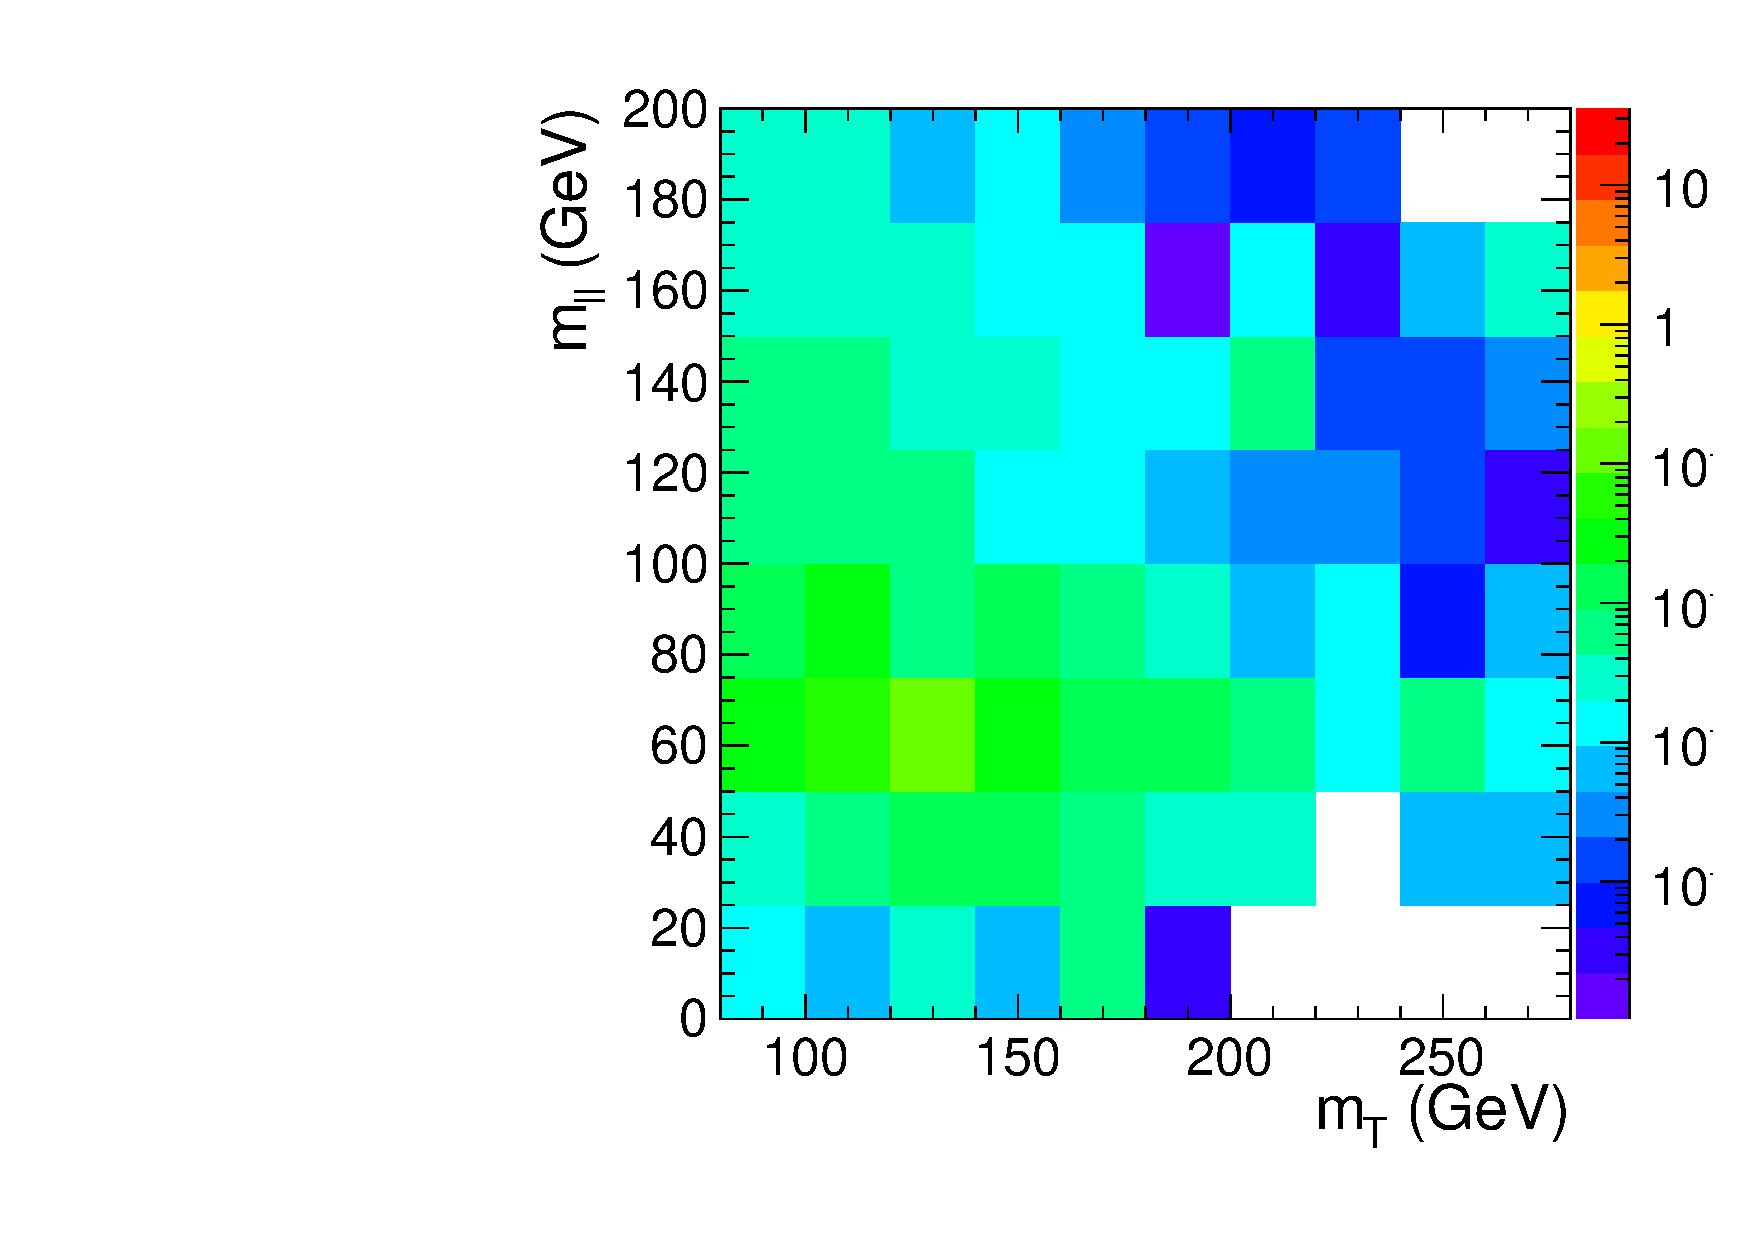
\includegraphics[width=.35\textwidth]{figures/templates/Zjets_2D_mH200_0j_of.pdf}
	}
	\subfigure[Zjets statistical uncertainty]{
	\centering
	\label{subfig:template_Zjetserr_200}
		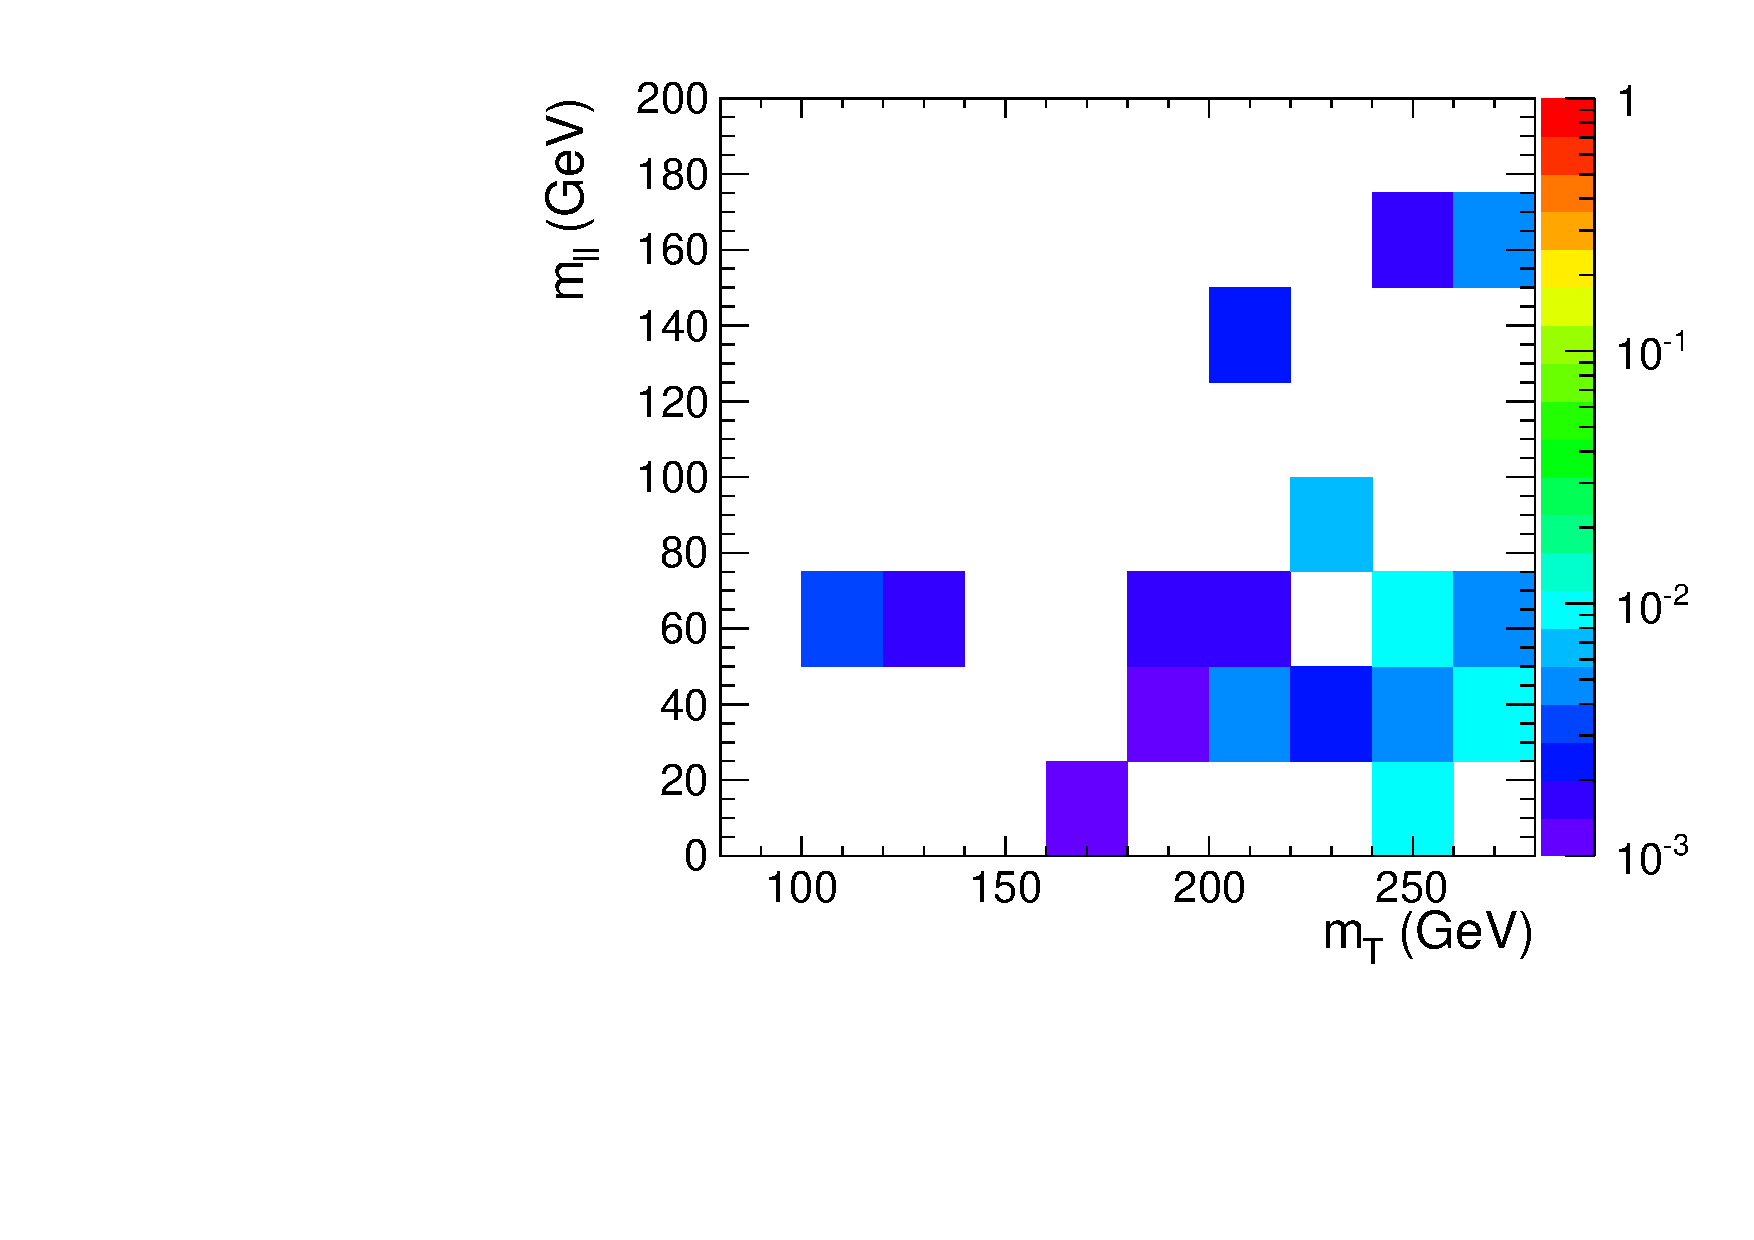
\includegraphics[width=.35\textwidth]{figures/templates/Zjetserr_2D_mH200_0j_of.pdf}
	}

	%
	\centering
	\subfigure[Wgamma]{
	\centering
	\label{subfig:template_Wgamma_200}
		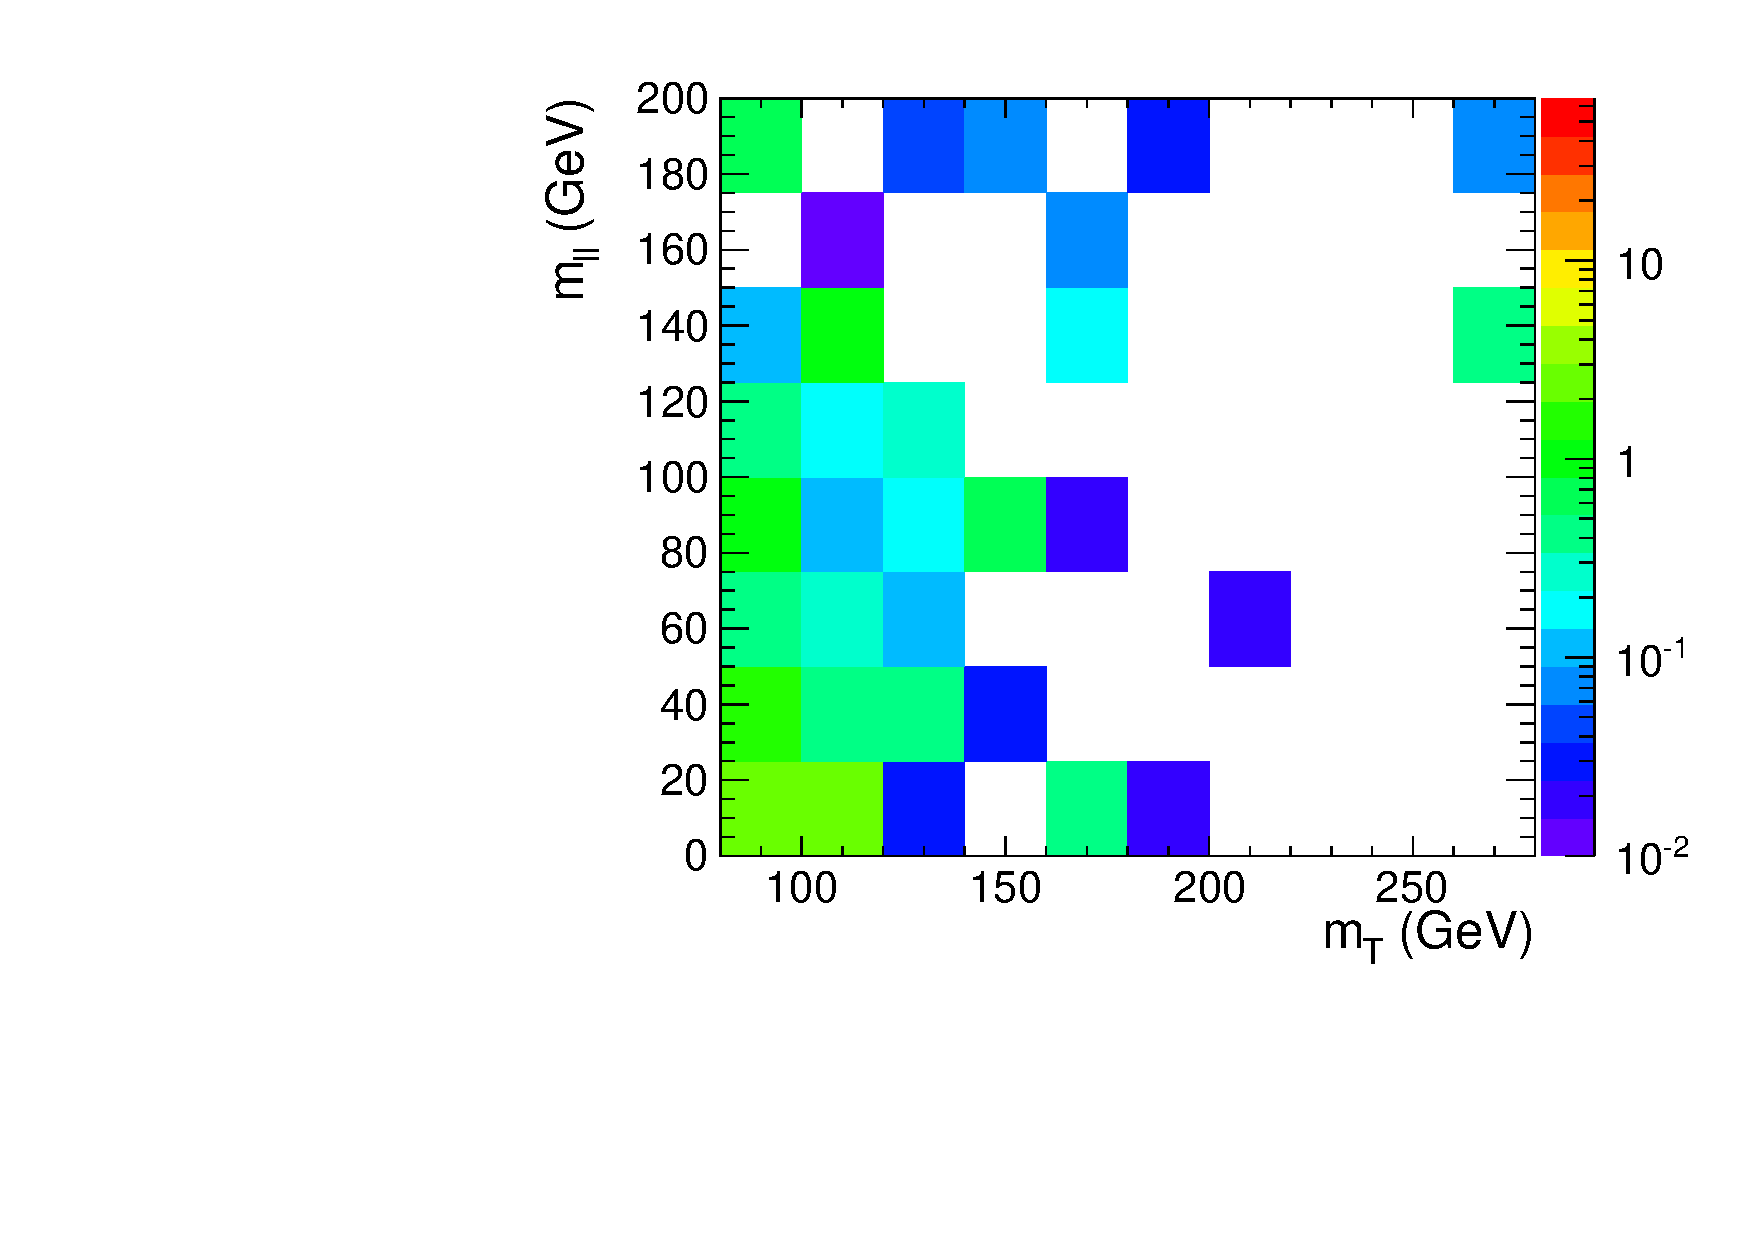
\includegraphics[width=.35\textwidth]{figures/templates/Wgamma_2D_mH200_0j_of.pdf}
	}
	\subfigure[Wgamma statistical uncertainty]{
	\centering
	\label{subfig:template_Wgammaerr_200}
		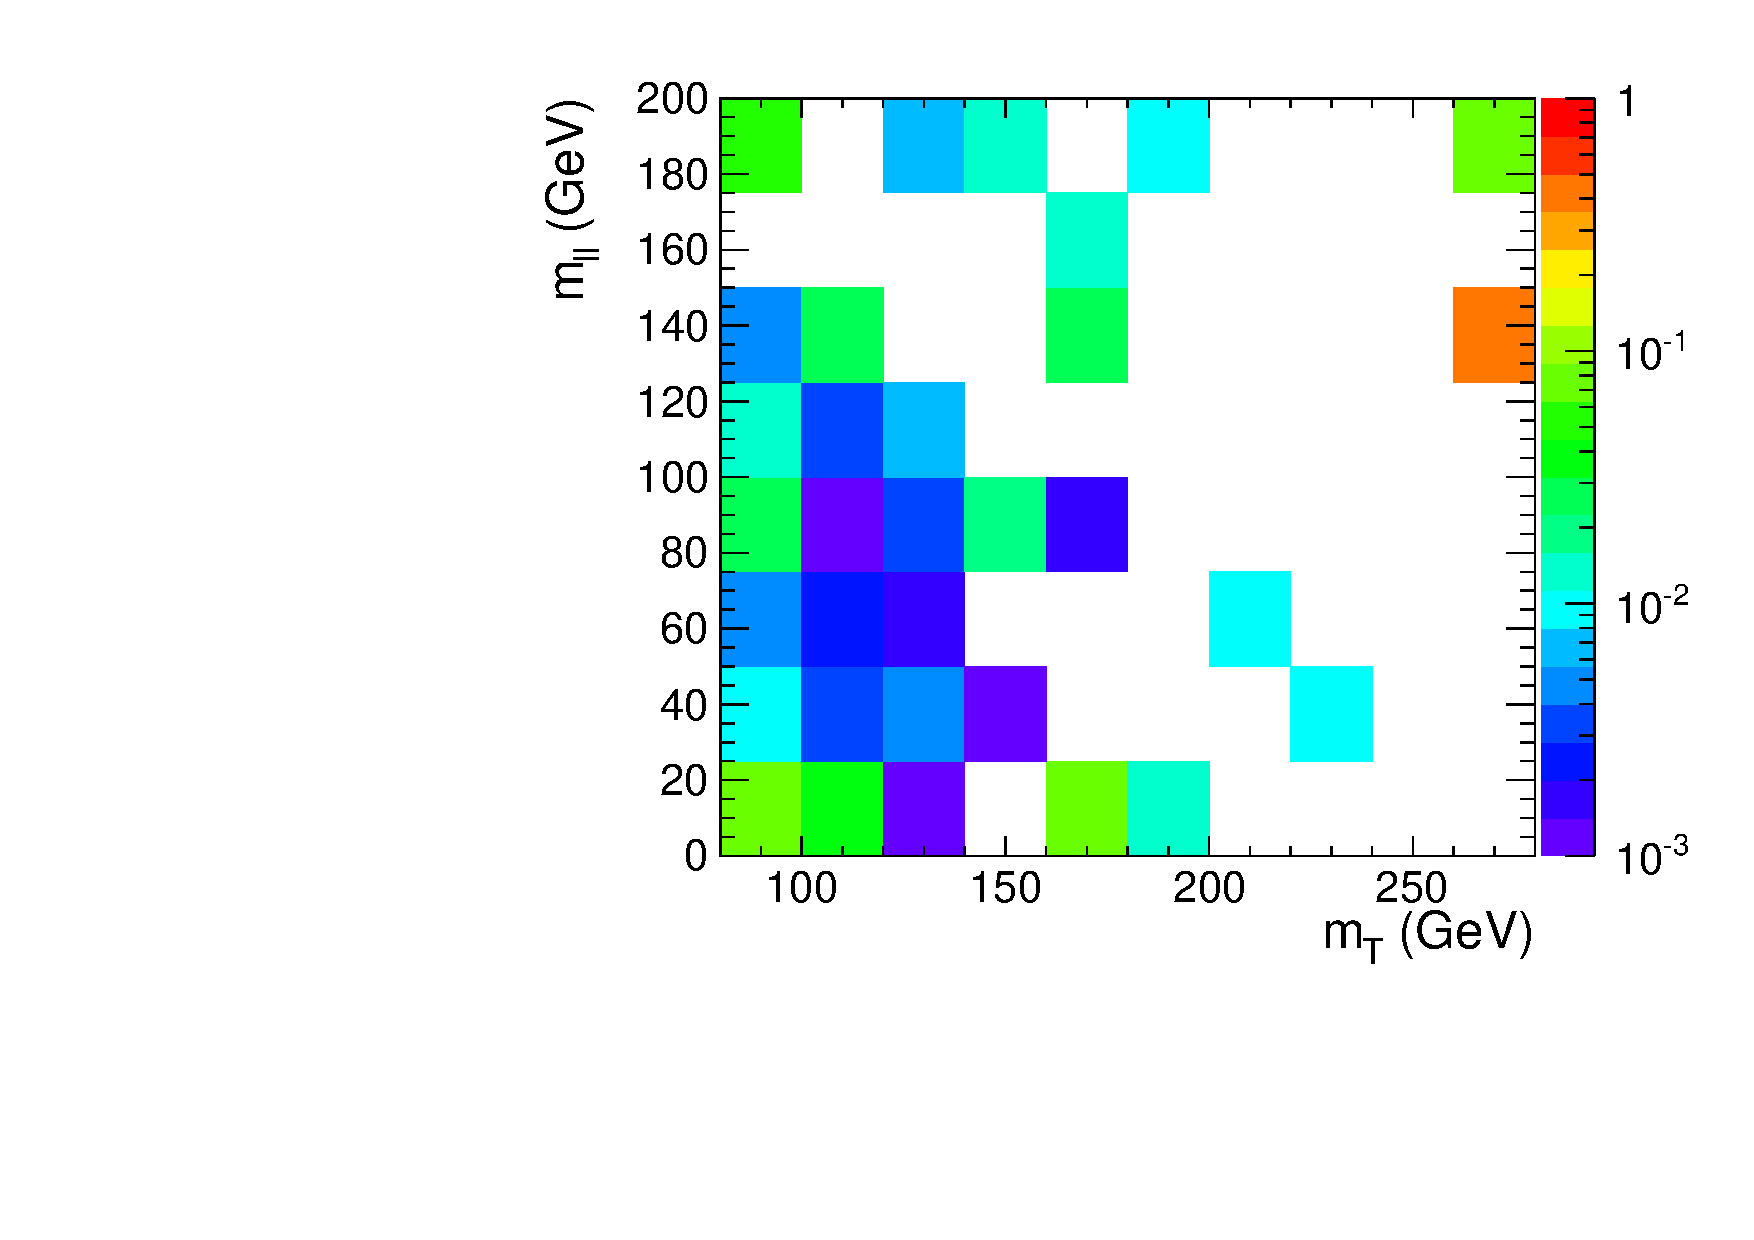
\includegraphics[width=.35\textwidth]{figures/templates/Wgammaerr_2D_mH200_0j_of.pdf}
	}

	\caption{2D templates at \mHi = 200 \GeV} 
	\label{fig:templates_200_3}

\end{figure} 

\begin{figure}[!hbtp]
	
	%
	\centering
	\subfigure[Stacked unrolled template linear]{
	\centering
	\label{subfig:template_unroll_stack_lin}
		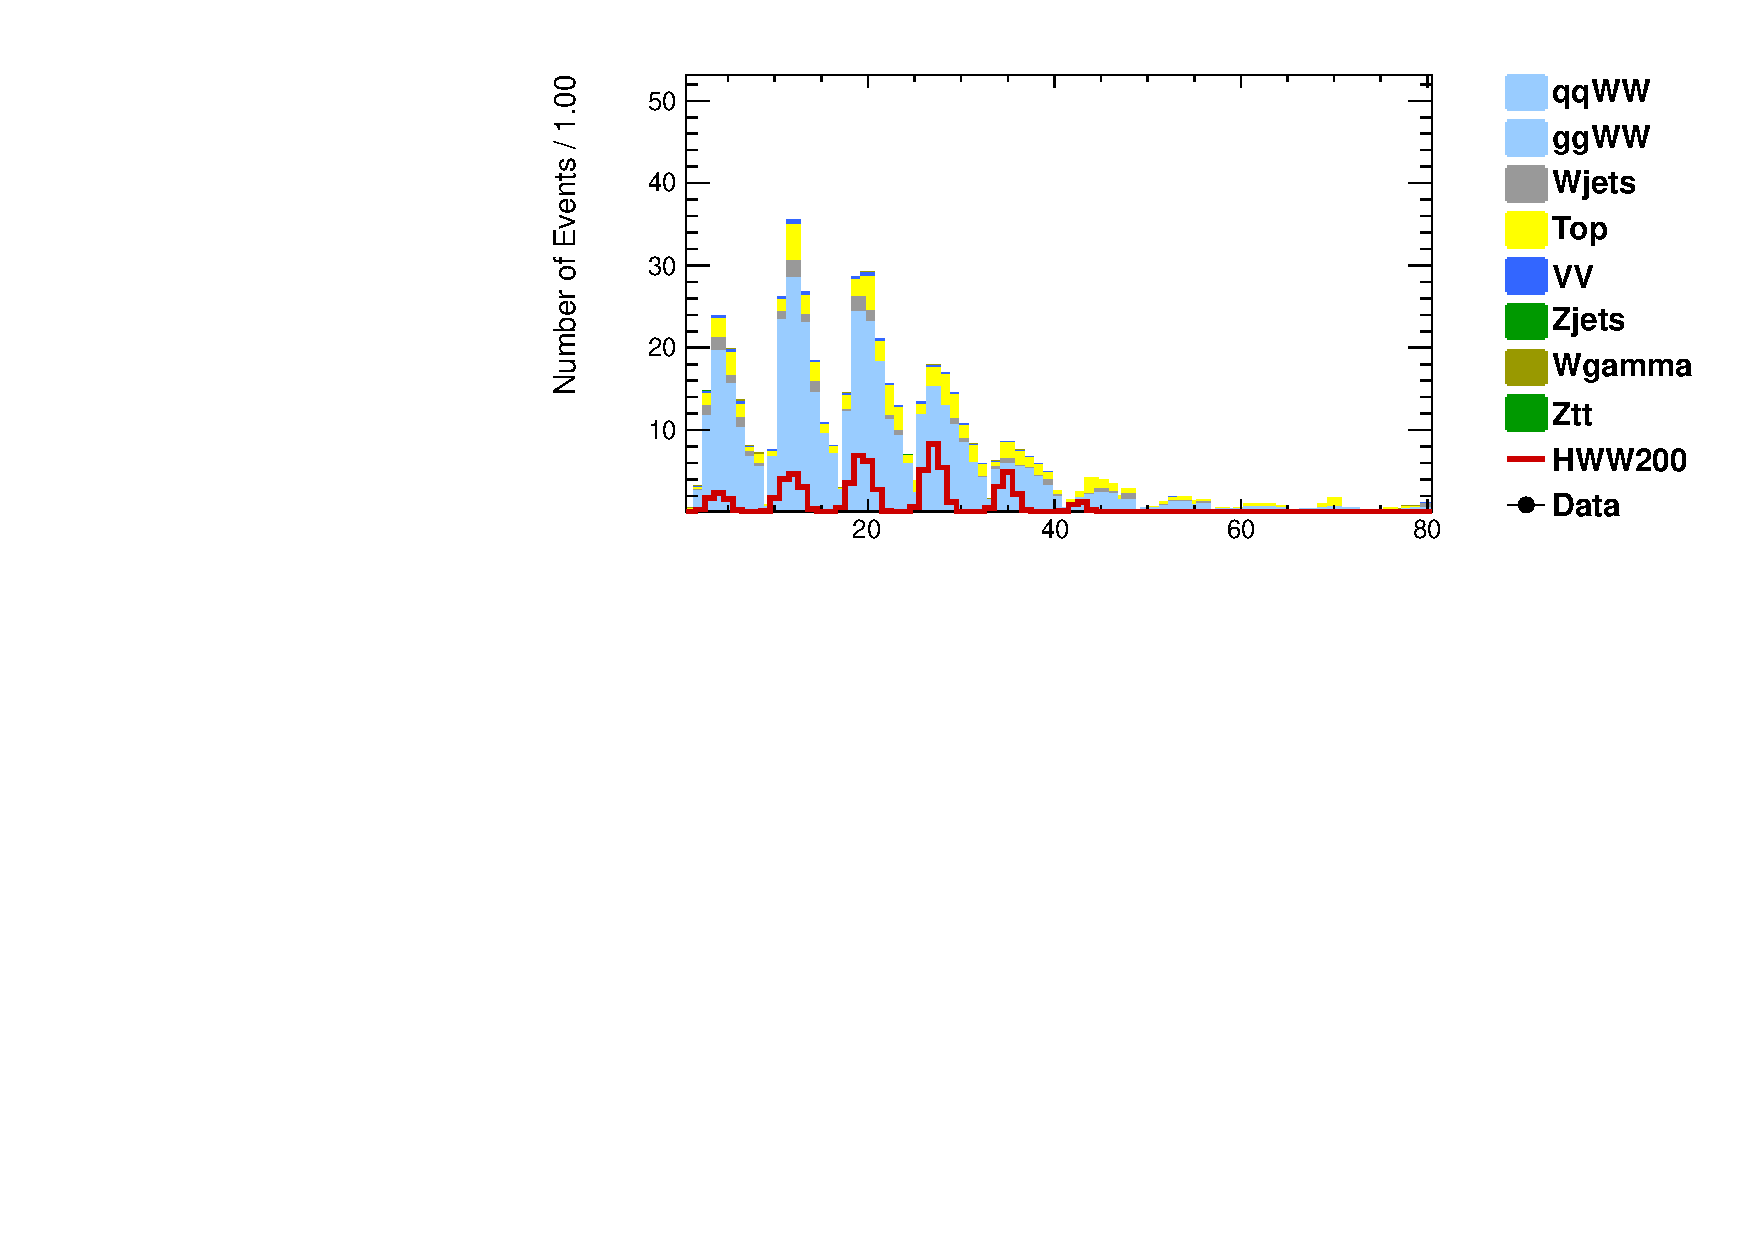
\includegraphics[width=.45\textwidth]{figures/templates/2D_mH200_0j_of_stack_lin.pdf}
	}
	\subfigure[Overlaid unrolled template linear]{
	\centering
	\label{subfig:template_unroll_overlay_lin}
		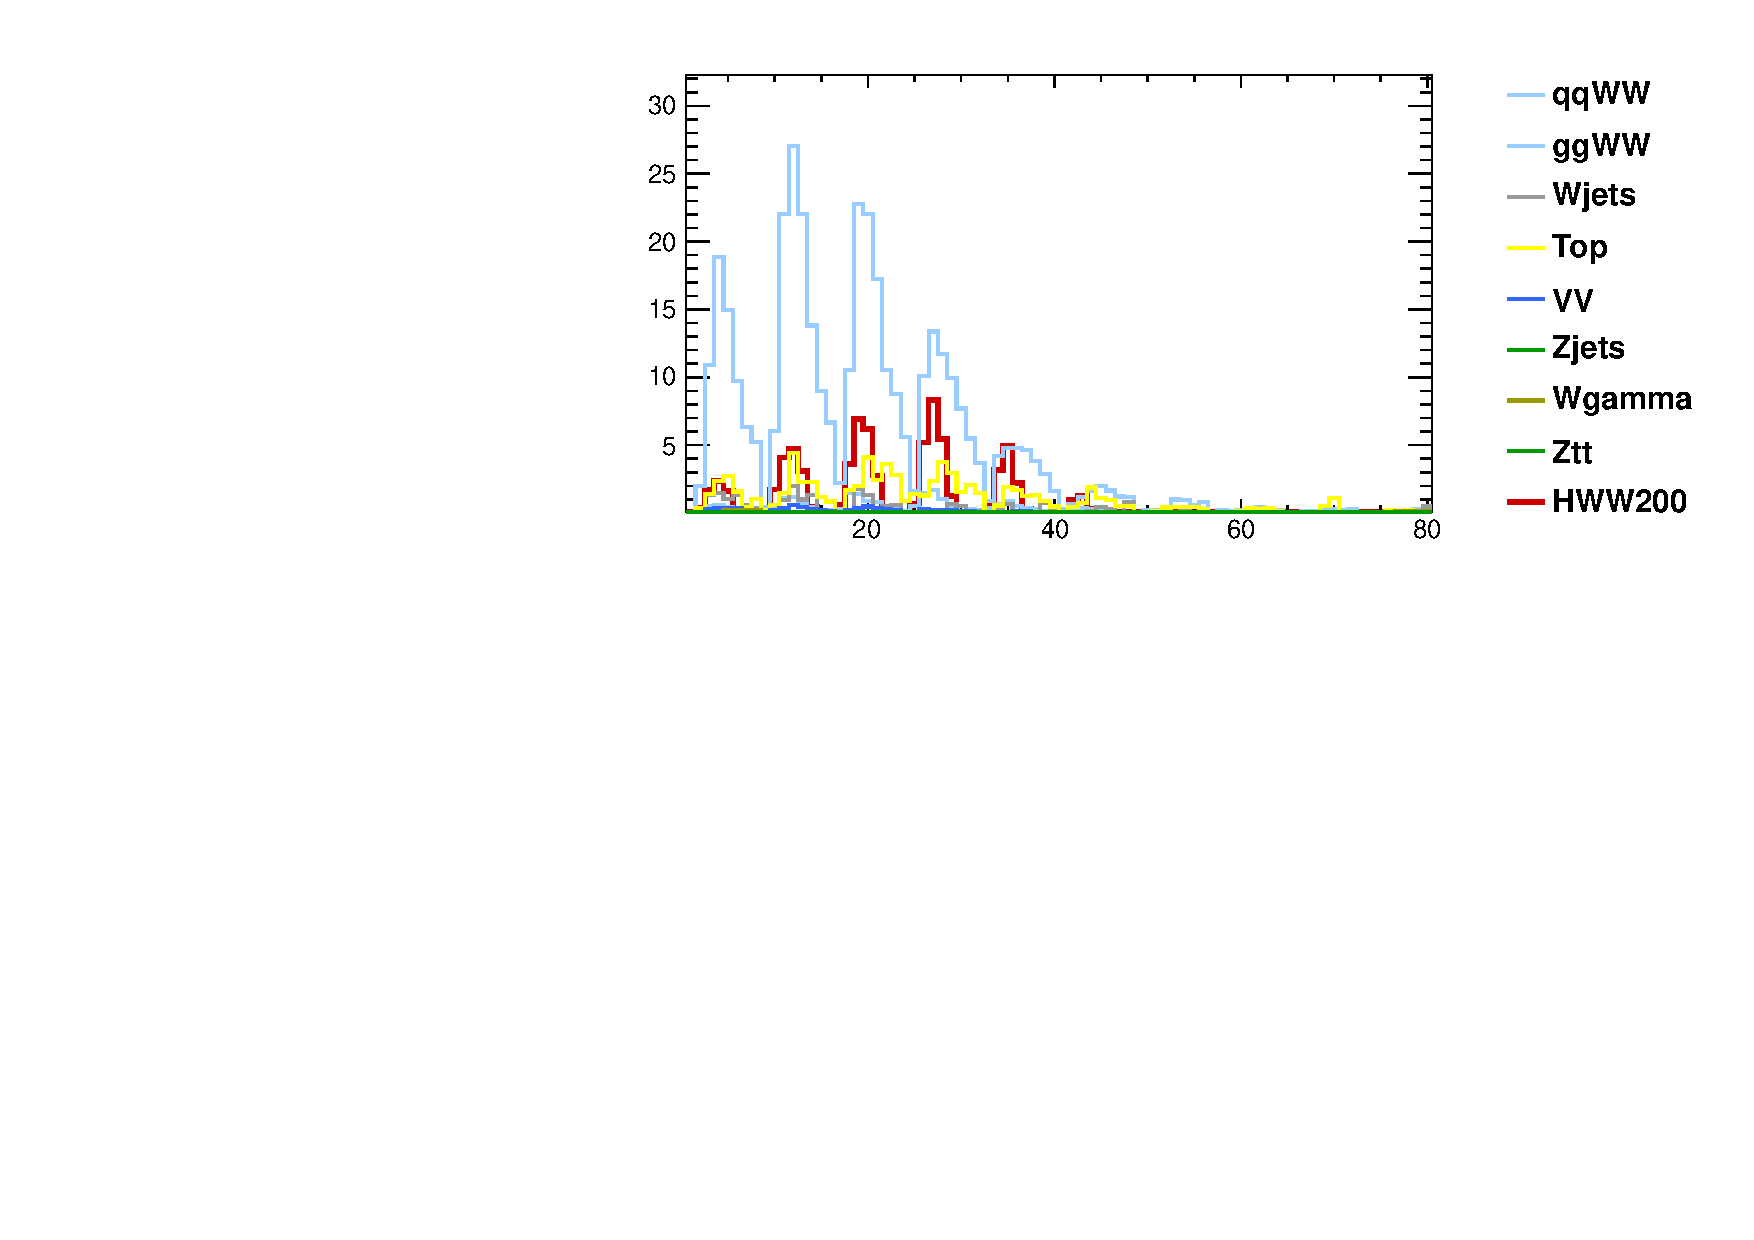
\includegraphics[width=.45\textwidth]{figures/templates/2D_mH200_0j_of_overlay_lin.pdf}
	}

	%
	\centering
	\subfigure[Stacked unrolled template in log scale]{
	\centering
	\label{subfig:template_unroll_stack_log}
		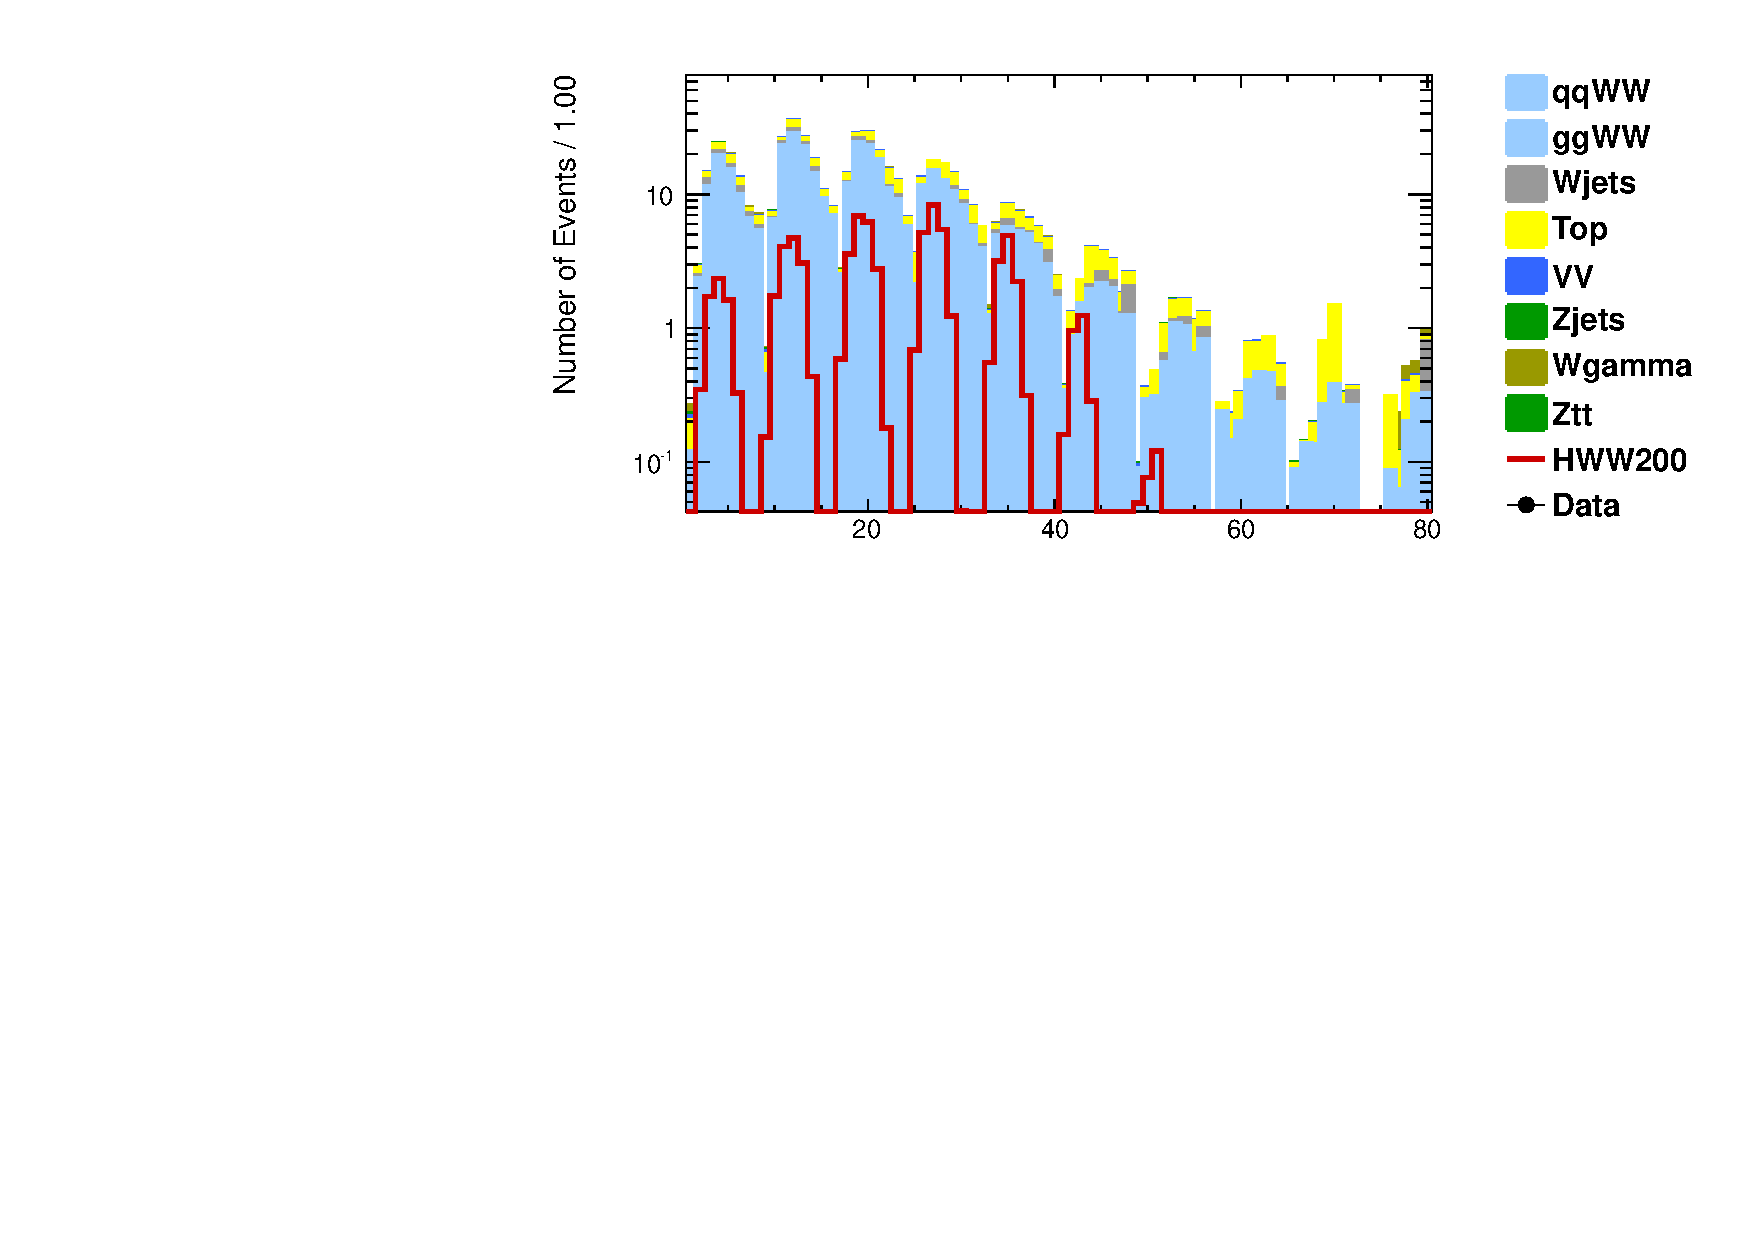
\includegraphics[width=.45\textwidth]{figures/templates/2D_mH200_0j_of_stack_log.pdf}
	}
	\subfigure[Overlaid unrolled template in log scale]{
	\centering
	\label{subfig:template_unroll_overlay_log}
		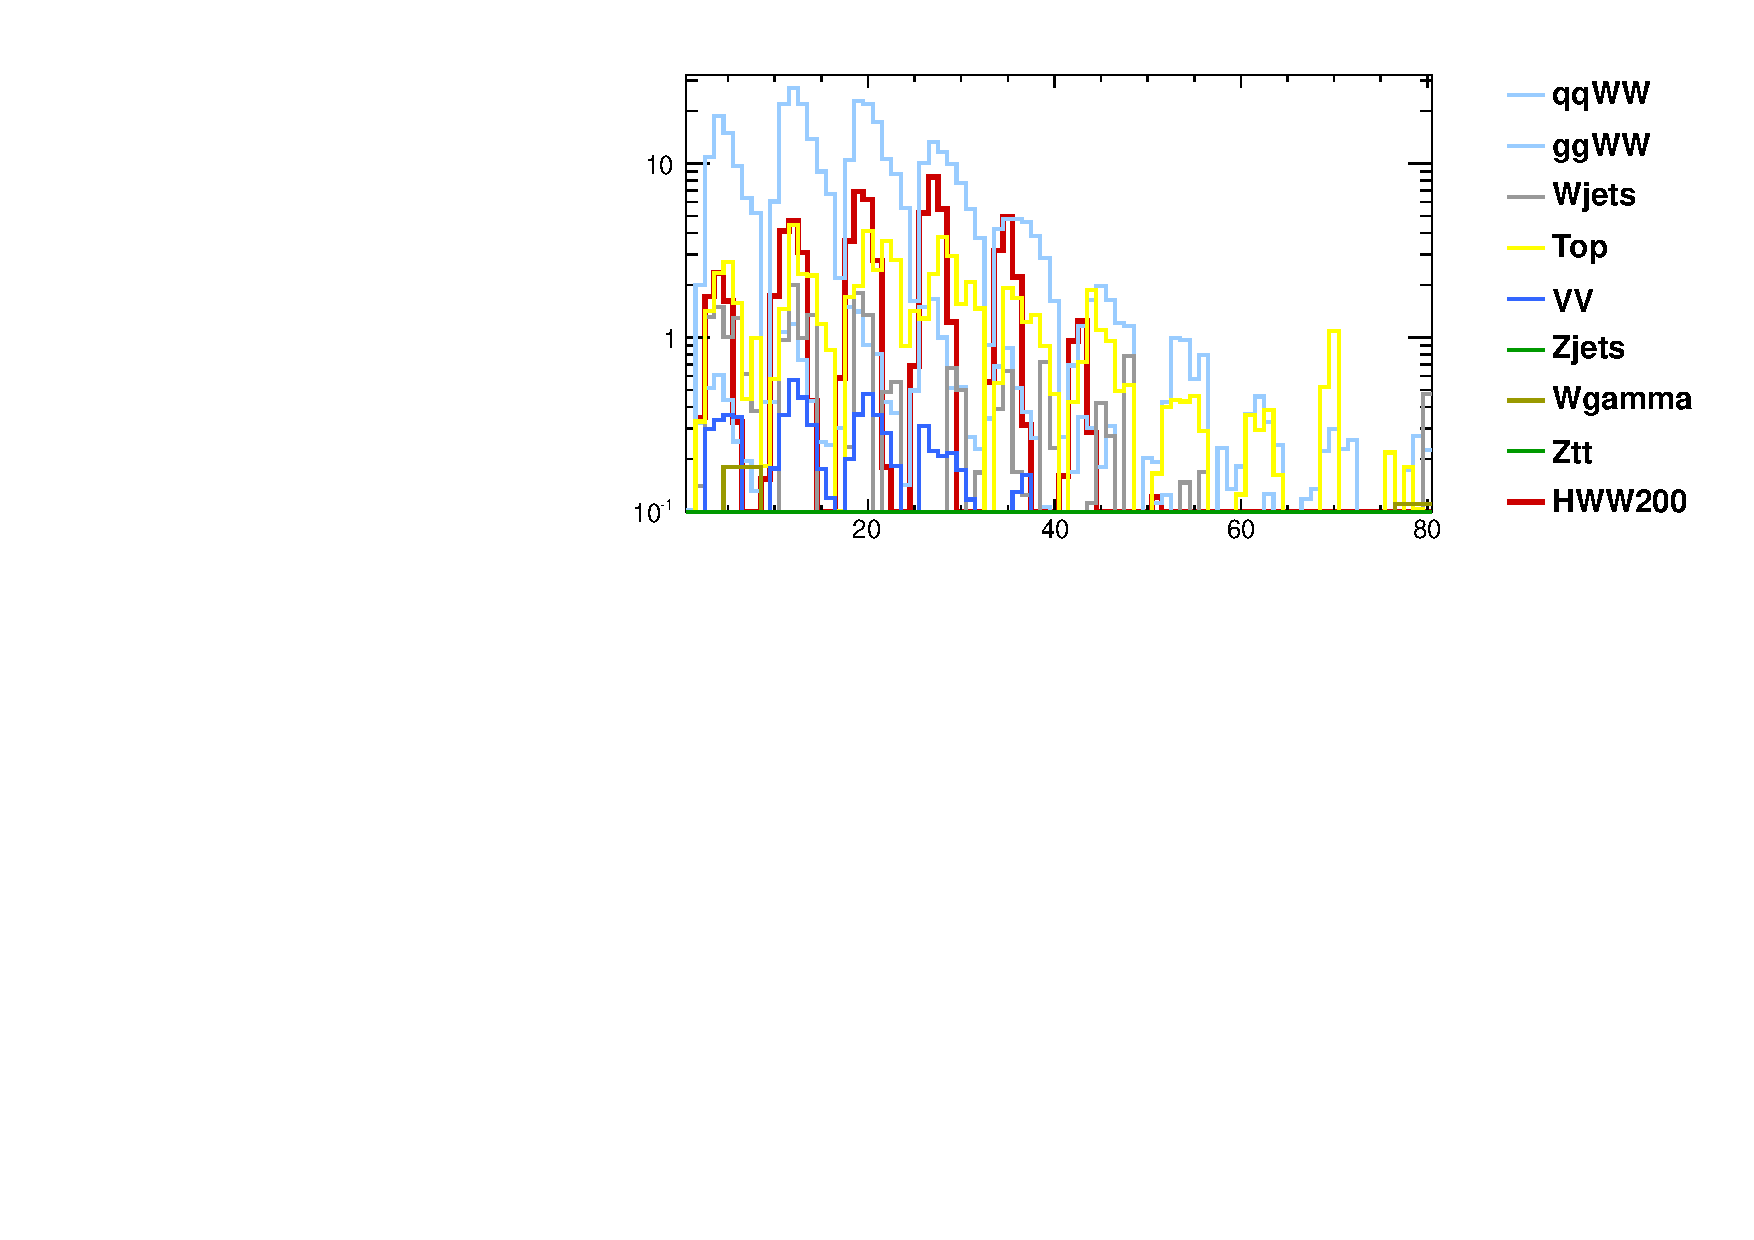
\includegraphics[width=.45\textwidth]{figures/templates/2D_mH200_0j_of_overlay_log.pdf}
	}

	\caption{Unrolled templates at \mHi = 200 \GeV} 
	\label{fig:templates_200_unroll}

\end{figure} 
